\documentclass[a4paper,11pt,twoside,openright]{Thesis}

\usepackage[phd]{ThesisTemplate} 

\setcounter{secnumdepth}{3} % show subsubsection numbers

\putTitle{Measurement of}
\putAuthor{Minori FUJIMOTO}{Department of Physics, Ochanomizu University}
\date{\today}

\begin{document}
\maketitle
\frontmatter
\putAbstract{inputs/abst}
\tableofcontents

\mainmatter
\chapter{Introduction}
The probe of the electroweak symmetry breaking is one of the most inportant topics of the LHC experiments.
In the SM, EWSB is explained by the Brout–Englert–Higgs mechanism \cite{}. 
Although many measurements have been made of the properties of the Higgs boson, more information is needed for a complete picture of EWSB. Vector-boson scattering (VBS) is a key probe of EWSB, since it is sensitive to interactions between the longitudinal components of the gauge bosons.

ATLAS and CMS have presented results of VBS searches during the Run-II \cite{STDM-2017-19,CMS-SMP-20-001} and the observation of the SM VBS process has been claimed by the ATLAS collaboration.

A common way of parameterizing BSM physics in VBS is through a low-energy effective theory \cite{Longhitano:1980tm}. Such an approach avoids having to choose a specific BSM theory, and is particularly well suited if the energy scale of the BSM physics is too high for the new resonances of the theory to be observed directly. In this kind of framework, VBS can be modified by anomalous quartic gauge couplings (aQGCs). 
%Searches for aQGCs have been performed by the LEP experiments \cite{delphi1, L3_1, L3_2, opal1, opal2, opal3}, D0 \cite{d0aQGC}, and the LHC experiments both at 8 \TeV
\cite{STDM-2013-06,STDM-2013-05,STDM-2014-02, STDM-2014-01, STDM-2014-05, STDM-2015-07,
STDM-2015-09, CMS-SMP-13-009, CMS-SMP-13-015, CMS-FSQ-13-008}
and 13 \TeV
%\cite{STDM-2017-23, STDM-2017-24, STDM-2017-20, STDM-2017-06, STDM-2017-26, STDM-2017-19}
.
A typical prediction of aQGCs is an enhancement of the VBS cross-section at high transverse momentum ($p_T$) of the vector bosons and at high invariant mass of the diboson system.

Experimentally, the VBS signature is characterized by the presence of a pair of vector bosons (W, Z, or $\gamma$) and two forward jets with a large separation in rapidity and a large dijet invariant mass. Previous searches for aQGCs in VBS have focused on channels involving leptonic boson decays ($W(l\nu)$ and $Z(ll)$)~\footnote{Unless otherwise noted, $\ell=e,\mu$ in this paper.} and photons.
The leptonic channels, i.e. $V(qq')Z(\nu\nu)$, $V(qq')W(l\nu)$ and $V(qq')Z(ll)$ (V = W, Z), however, offer some interesting advantages. The $V(qq')$ branching fractions are much larger than the leptonic branching fractions. In addition, the use of jet substructure techniques allows good reconstruction efficiency in the high-pT region, which is the most sensitive to aQGCs.
The main challenge of the simpleton channels is the presence of large backgrounds from $W + jets$, $Z + jets$ and $t\bar{t}$ events. These backgrounds make a SM VBS measurement in this channel very challenging because it is difficult to achieve a favorable signal-to-background ratio. On the other hand, an aQGC search is less sensitive to these backgrounds because it is possible to find regions of phase space where the aQGC signal is greatly enhanced over the SM processes, resulting in large signal-to-background ratios. This motivates a search for aQGCs in the semi-leptonic channels.


\chapter{Theoretical Overview}

This chapter describes the physics backgrounds of the semileptonic VBS analysis.

\section{The Standard Model}

The Standard Model (SM) represents a description of the elementary particles and their interactions.
It is proved successful in explaining the results of existing experimental results so far, and predicting the later results.
All particles predicted by SM has been confirmed its existence, most recently the Higgs boson found with ATLAS and CMS.
The SM predicts the existence of elementary particles which form the matter, which is fermion, classified into leptons and quarks.
The interactions of them are described by the gauge field mediated by the exchange of particles named bosons.
With these particles the model is describing three of the four known forces, which are the electromagnetic, the weak and the strong force. 
The theoretical description is given with the Quantum Field Theory (QFT) framework. The gauge invariance, which is the invariance of the local gauge transformation is the key of the framework. The underlying symmetry is described with the gauge group, SU(3)$_C \times$ SR(2)$_L \times$ U(1)$_Y$, which described in this section. These underlying structure of gauge theories can be described by Lie groups.

\subsection{Particle Content}
The 17 fundamental particles, which means particles with no substructure are considered in SM as the Figure~\ref{fig:SM} shows.
\begin{figure}[tbp]
\begin{center}
%\subfigure[]{
 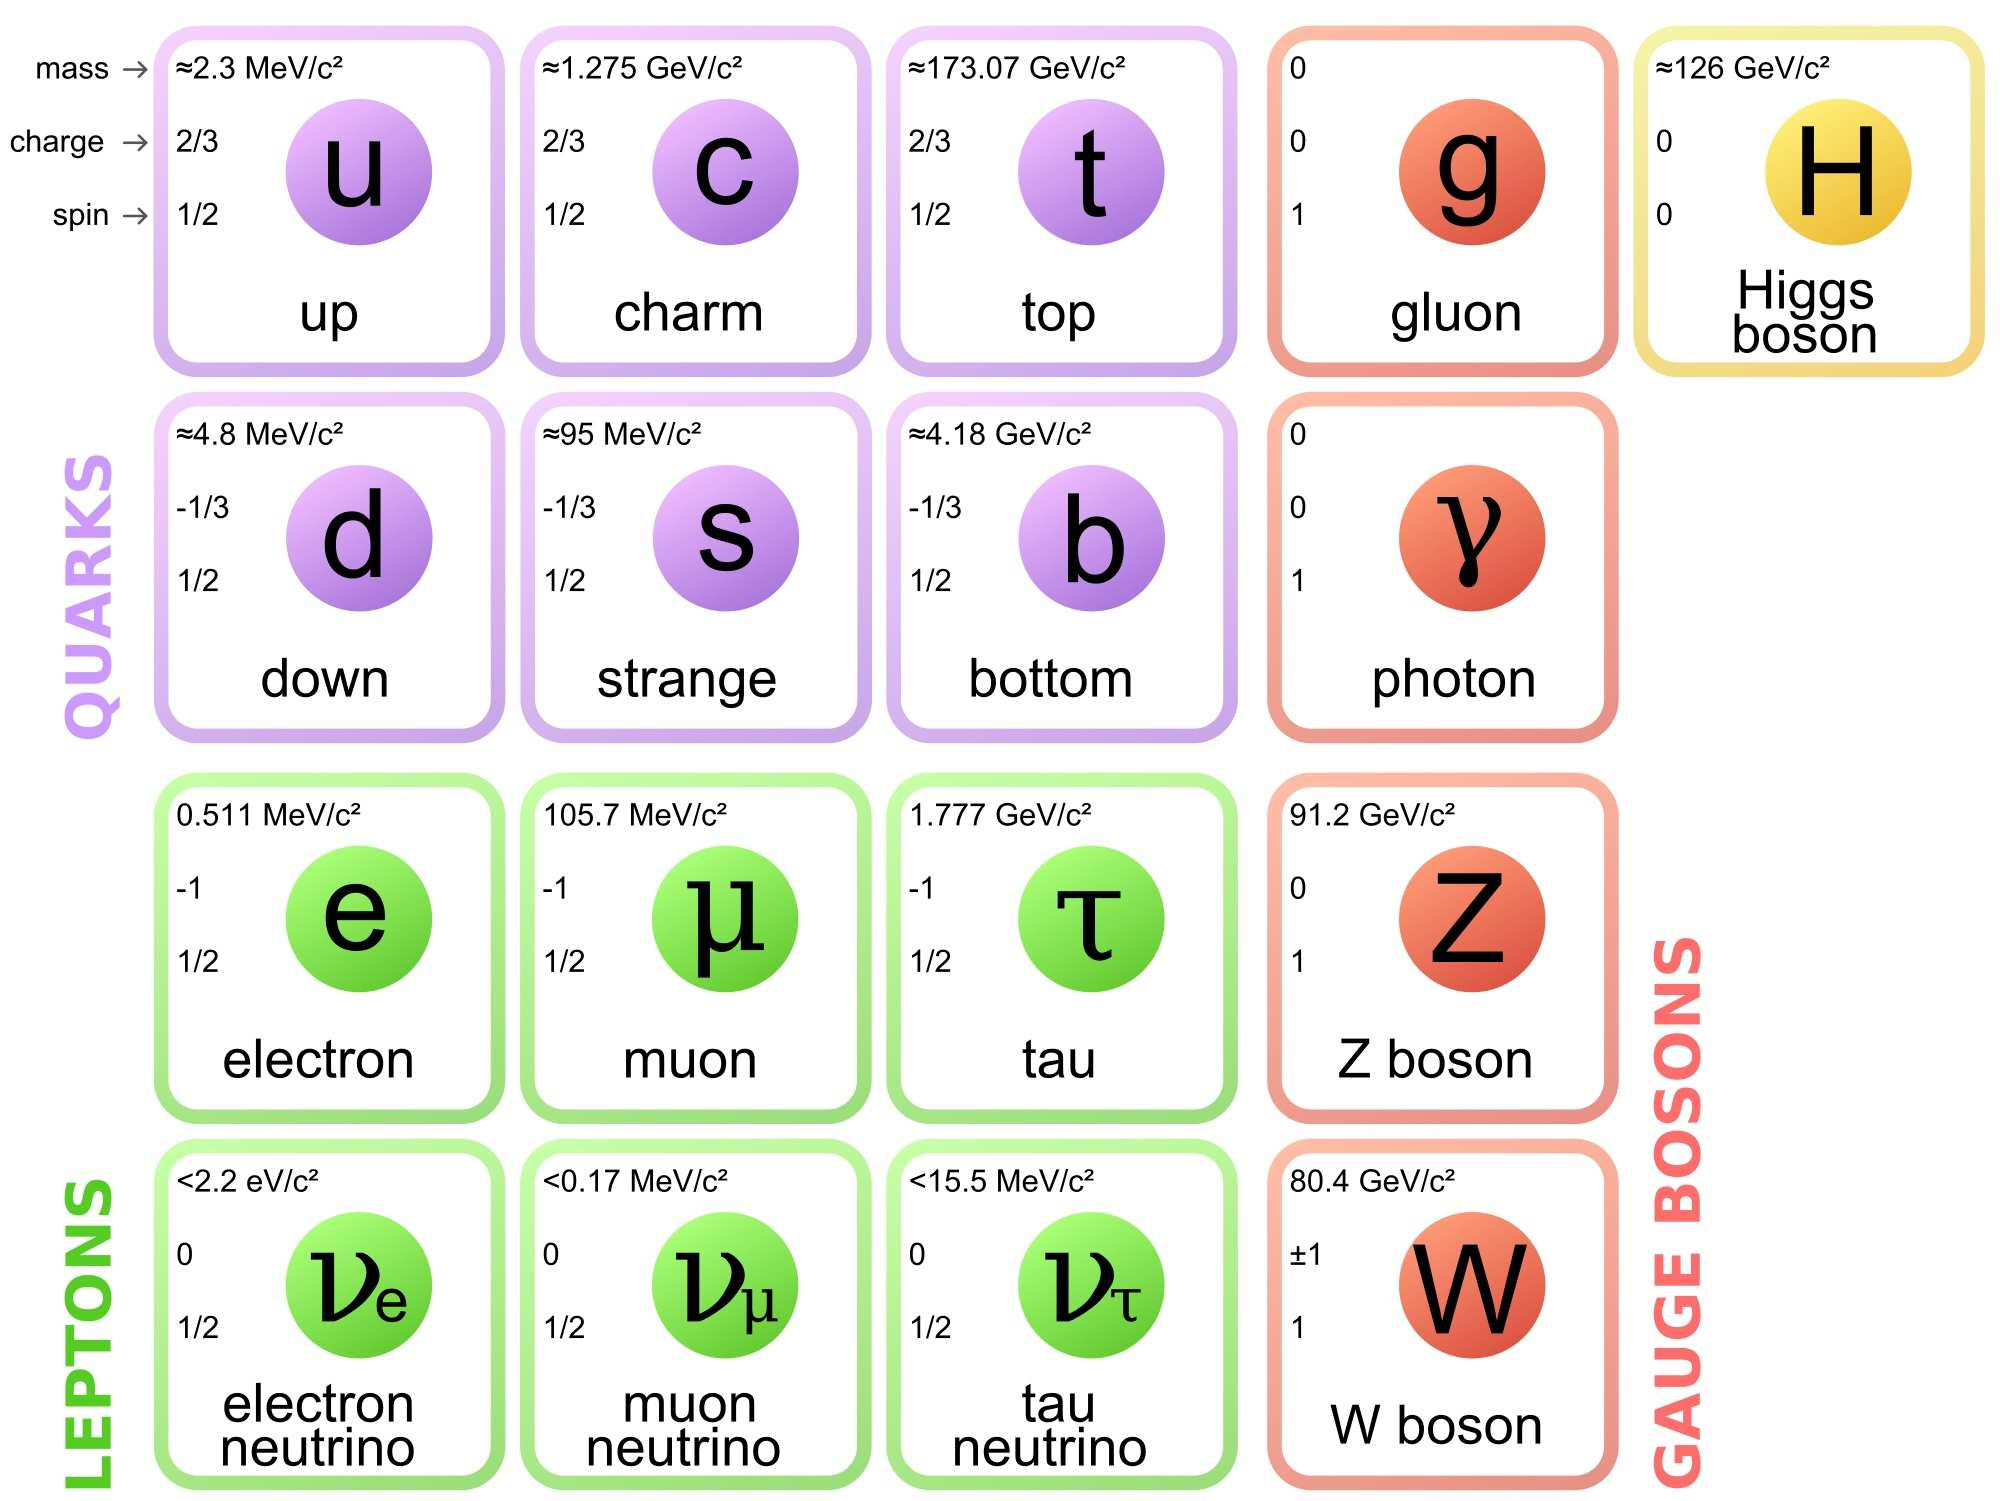
\includegraphics[width=0.85\textwidth,keepaspectratio]{figures/SM}
%}
\caption{
All particles exist in the SM %\ref{}
}
\label{fig:SM}
\end{center}
\end{figure}

There are two types of particles described in details below:
\begin{itemize}
    \item Fermion \\
    Fermions are the elementary particles with spin 1/2. There are three generations called flavors. The generations are classified only by the particle masses, increasing from first generation to the third generation. They are two types of fermions, quarks and leptons, each has 6 particles. Leptons do not act through the strong force, unlike the quarks.
    \item Boson \\
    Bosons are integer-spin particles and mediate the interaction of the fermions.
    The photons ($\gamma$) are mediator of the electromagnetic forces. The photons are massless and stable, and the electromagnetic force can be interact with infinite ranges. The photons interact with every particles with electric charges.The gluons (g) are the intermediate particles of the strong force. Also gluons are massless, and interact with the quarks and the gluons itselves.The W$^\pm$ and the Z bosons carry weak force. They are massive particles and interact with all particles carrying the weak hyper charges. The W$^\pm$ can change the flavor of the quarks. 
\end{itemize}

\subsection{SM Lagrangian}
\label{ch:Lagrangian}
The SM Lagrangian and its origin is to be shown here in this subsection. 
The Standard Model consists of several components as discribed in the following subsections. They are mathematically described as the Lagrangian density, $\mathcal{L}$, which is denoted as Lagrangian in the following.\\

\noindent\textbf{\sf{Quantum Electro Dynamics (QED)}} \\ 
The QED describes the dynamics of fermions and their electromagnetic interactions.

The free fermion with the spin 1/2 is described by the Lagrangian\\
\begin{equation}
\label{eqn:QED}
\mathcal{L}=i \bar{\psi} \gamma^{\mu} \partial_{\mu} \psi-m \bar{\psi} \psi
\end{equation}
The $\psi$ here is the spinor of the fermion field, $\gamma^{\mu}$  ($\mu$ = 0,1,2,3) is the Dirac gamma 4$\times$4 matrix. $\partial_{\mu}$ = $\frac{\delta}{\delta x_{\mu}}$ are the partial derivatives, and the $\bar{\psi}=\psi^{\dagger} \gamma^{0}$.
For describing the equation of motion, the Dirac equation is given for $\psi$:
\begin{equation}
\left(i \gamma^{\mu} \partial_{\mu}-m\right) \psi=0
\end{equation}
The Lagrangian needs to be invariant with the "local" gauge transformation, i.e. the guage transformation parameter depends on x:
\begin{equation}
\psi(x) \rightarrow \psi^{\prime}(x)=e^{i \alpha(x)} \psi(x)
\end{equation}
where the local phase is given by $\alpha(x)$, depends on space and time. 
This transformation form the abelian unitary group U(1) with e$^{i\alpha(x)}$ can be written as the 1$\times$1 matrix with $U^{\dagger} U=1$.
The first term of the Lagrangian (\ref{eqn:QED}) is calculated and it is not invariant under this transformation:
\begin{equation}
\partial_{\mu} \psi \rightarrow \partial_{\mu} \psi^{\prime}=e^{i \alpha(x)} \partial_{\mu} \psi+i e^{i \alpha(x)} \psi \partial_{\mu} \alpha(x)
\end{equation}
The requirement of the invariance leads us to introduce an additional field A$_\mu$, transforming as:
\begin{equation}
A_{\mu} \rightarrow A_{\mu}^{\prime}=A_{\mu}+\frac{1}{e} \partial_{\mu} \alpha(x)
\end{equation}
where e is a coupling constant, which is elementary electric charge. 
and $\partial_{\mu}$ is replaced with the covariant derivative D$_\mu$:
\begin{equation}
D_{\mu}=\partial_{\mu}-i e A_{\mu}
\end{equation}
Then the derivative part can be replaced with:
\begin{equation}
D_{\mu} \psi \rightarrow D_{\mu}^{\prime} \psi^{\prime}=e^{i \alpha(x)} D_{\mu} \psi
\end{equation}
which leads the Lagrangian as:
\begin{equation}
\begin{aligned}
\mathcal{L} &=i \bar{\psi} \gamma^{\mu} D_{\mu} \psi-m \bar{\psi} \psi \\
&=\bar{\psi}\left(i \gamma^{\mu} \partial_{\mu}-m\right) \psi+e \bar{\psi} \gamma^{\mu} \psi A_{\mu}
\end{aligned}
\end{equation}
The Lagrangian now restore the invariance with the gauge field A$_\mu$. By using the strength tensor $F_{\mu \nu}=\partial_{\mu} A_{\nu}-\partial_{\nu} A_{\mu}$, the Lagrangian of QED is defined as:
\begin{equation}
\label{eqn:QEDLagrangian}
\mathcal{L}_{\mathrm{QED}}=i \bar{\psi} \gamma^{\mu} \partial_{\mu} \psi-m \bar{\psi} \psi+e \bar{\psi} \gamma^{\mu} \psi A_{\mu}-\frac{1}{4} F_{\mu \nu} F^{\mu \nu}
\end{equation}
The Lagrangian is invariant under the U(1)$_{EM}$ local gauge transformations of fields. The field A$_\mu$ is identified as photon, and the invariance forbids the introduction of a mass term of the A$_\mu$, of the form of $\frac{1}{2}m^2 A_\mu A^\mu$. The photon is requested to be massless, which agrees with all experiment results.
\\

\noindent\textbf{\sf{Quantum Chromo Dynamis (QCD))}} \\ 
The QCD describes the strong force interactions between quarks and gluons. The concept of the required invariance is similar to the QED, while an additional degree of freedom is introduced: the charge denoted as color, which is red (r), green(g), and blue(b). The Dirac spinor is replaced with vector of three spinors for quarks:
\begin{equation}
\psi=\left(\begin{array}{c}
\psi_{r} \\
\psi_{g} \\
\psi_{b}
\end{array}\right)
\end{equation}
The Lagrangian of QCD is described as:
\begin{equation}
\mathcal{L}_{\mathrm{QCD}}=i \bar{\psi} \gamma^{\mu} \partial_{\mu} \psi-m \bar{\psi} \psi-g_{s}\left(\bar{\psi} \gamma^{\mu} \frac{\lambda_{a}}{2} \psi\right) G_{\mu}^{a}-\frac{1}{4} G_{\mu \nu}^{a} G_{a}^{\mu \nu}
\end{equation}
with the gauge fields $G_{\mu}^{a}$ (a = 1,2,...,8) represents the gluons.
QED is an Abelian gauge theory since the underlying Lie group is the Abelian group U(1)$_{EW}$. For QCD, the underlying group is the non-Abelian group SU(3)$_C$, whose generators are T$_a$ = $\lambda_{a}/2$. $\lambda_{a}$ are callsed Gell-Mann matrices. They satisfy the commutator relation:
\begin{equation}
\left[\frac{\lambda_{a}}{2}, \frac{\lambda_{b}}{2}\right]=i f_{a b c} \frac{\lambda_{c}}{2}
\end{equation}
g$_s$ denotes the strong coupling constatnt, and $G_{a}^{\mu \nu}$ is the field strength tensor, written as:
\begin{equation}
G_{\mu \nu}^{a}=\partial_{\mu} G_{\nu}^{a}-\partial_{\nu} G_{\mu}^{a}-g_{s} f_{a b c} G_{\mu}^{b} G_{\nu}^{c}
\end{equation}
The non-Abelian group structure produces the last term of the field strength, which enables the gluons to interact with themselves differently from QED. Gluons are also requested to be massless from the gauge transformation of the fields.
%The whole Lagrangian for QCD??
\\ \\

\noindent\textbf{\sf{ElectroWeak Model}} \\
It is shown by experiments that the weak interaction only acts on left-handed fermions. In the electroweak model, the SU(2)$_L \times$ U(1)$_Y$ symmetry is conserved. Here the left-handed fermions are assigned to SU(2)$_L$ doublets with weak isospin I = 1/2, and gauge field W$^a_\mu$. The right-handed fermions are assigned to  U(1)$_Y$ singlets with weak isospin I = 0, and gauge field B$_\mu$.
%table of the quantum numbers
The left-handed doublets and right-handed singlet denote as $\chi_{L}$ and $\psi_{R}$ ,respectively. Specifically $\chi_{L}$ is written as 
$
\left(\begin{array}{c}
\nu_{L} \\
e_{L}
\end{array}\right)
$
for the leptons of the first generation, and $\psi_{R}$ is written as $(e_R)$.
For the quarks of the first generation, $\chi_{L}$ is 
$
\left(\begin{array}{c}
u_{L} \\
d_{L}
\end{array}\right)
$
and $\psi_{R}$ is $(u_R)$ and $(d_R)$.




These behave with local phase transformations as:
\begin{equation}
\begin{aligned}
\chi_{L}(x) \rightarrow \chi_{L}^{\prime}(x) &=e^{i \alpha_{a}(x) \tau_{a}} e^{i \beta(x) Y} \chi_{L} \\
\psi_{R}(x) \rightarrow \psi_{R}^{\prime}(x) &=e^{i \beta(x) Y} \psi_{R}
\end{aligned}
\end{equation}
where $\alpha_{a}(x)$ and $\beta(x)$ are the local phases, $\tau_{a}$ are the generators of SU(2)$_L$ with a = 1,2,3, and Y is the weak hypercharge operator of U(1)$_Y$. The covariant derivative is:
\begin{equation}
D_{\mu}=\partial_{\mu}+i g W_{\mu}^{a} \frac{\tau_{a}}{2}+i g^{\prime} B_{\mu} \frac{Y}{2}
\end{equation}
g here is the coupling constant of the SU(2)$_L$ gauge field written as $W_{\mu}^{a}$. $g^{\prime}$ is the coupling constant of the U(1)$_Y$ gauge field $B_{\mu}$.
The electroweak Lagrangian results in:
\begin{equation}
\mathcal{L}_{\mathrm{EW}}=i \overline{\chi_{L}^{i}} \gamma^{\mu} D_{\mu} \chi_{L}^{i}+i \overline{\psi_{R}^{i}} \gamma^{\mu} D_{\mu} \psi_{R}^{i}-\frac{1}{4} W_{\mu \nu}^{a} W_{a}^{\mu \nu}-\frac{1}{4} B_{\mu \nu} B^{\mu \nu}
\end{equation}
The field strength tensors are:
\begin{equation}
\begin{aligned}
W_{\mu \nu}^{a} &=\partial_{\mu} W_{\nu}^{a}-\partial_{\nu} W_{\mu}^{a}-g \epsilon_{a b c} W_{\mu}^{b} W_{\nu}^{c} \\
B_{\mu \nu} &=\partial_{\mu} B_{\nu}-\partial_{\nu} B_{\mu}
\end{aligned}
\end{equation}
where $\epsilon_{a b c}$ is an antisymmetric tensor, which is the structure constant of SU(2)$_L$. This term enables the $W_{a}^{\mu \nu}$ field to interact with themselves, while $B_{\mu}$ cannot self-interact.
The physical fields represents the W$^{\pm}$, Z bosons and photons are formed by linear combination of $W_{\mu \nu}^{a}$ and $B_{\mu \nu}$.
\begin{equation}
\begin{aligned}
W_{\mu}^{\pm} &=\frac{1}{\sqrt{2}}\left(W_{\mu}^{1} \mp i W_{\mu}^{2}\right) \\
Z_{\mu} &=\cos \theta_{W} W_{\mu}^{3}-\sin \theta_{W} B_{\mu} \\
A_{\mu} &=\sin \theta_{W} W_{\mu}^{3}+\cos \theta_{W} B_{\mu}
\end{aligned}
\end{equation}
where the $\theta_{W}$ = arctan ( g$^{\prime}$/g) represents the weak mixing angle, so called Weinberg angle. By rewriting the Lagrangian with physical fields and comparing the comparing the $A_{\mu}$ components with the QED Lagrangian (\ref{eqn:QEDLagrangian}), the relations between e and g, g$^{\prime}$ is obtained:
\begin{equation}
\begin{aligned}
e&=g \sin \theta_{W}=g^{\prime} \cos \theta_{W} \\
and \ \ Q&=I_{3}+\frac{Y}{2}
\end{aligned}
\end{equation}
The local gauge invariance forbid the introduction of the mass term of the 
The Lagrangian could include the mass terms of the bosons like $m^2_W W_\mu W^\mu$, while it is not invariant under $SU(2)_L \times U(1)_Y$ local transformations.
This statement that the local phase invariance in the electroweak model requests the fermions and bosons to be massless particles, is conflicted against the experimental results, where W$^{\pm}$ , Z bosons and fermions are found to be massive.
\\ \\
\noindent\textbf{\sf{Spontaneously Symmetry breaking}} \\ 
The conflict of the electroweak model of forbidding the masses of the fermions and boson can be solved by introducing a spontaneously symmetry breaking.
The mechanism is known as Brout-Englert-Higgs (BEH) mechanism or “Higgs mechanism” for short.

A complex scalar field, $\phi$, which is a weak isospin doublet is introduced as the Higgs field and has four degrees of freedom:
\begin{equation}
\label{eqn:higgsphi}
\phi=\left(\begin{array}{l}
\phi^{+} \\
\phi^{0}
\end{array}\right)=\frac{1}{\sqrt{2}}\left(\begin{array}{l}
\phi_{1}+i \phi_{2} \\
\phi_{3}+i \phi_{4}
\end{array}\right)
\end{equation}
The corresponding Lagrangian is written as:
\begin{equation}
\label{eqn:Higgs}
\mathcal{L}_{\text {Higgs }}=\left(D_{\mu} \phi\right)^{\dagger}\left(D^{\mu} \phi\right)-\mu^{2} \phi^{\dagger} \phi-\lambda\left(\phi^{\dagger} \phi\right)^{2}
\end{equation}
This is invariant under SU(2)$_l$ $\times$ U(1)$_Y$ phase transformation.
The potential of $\phi$ can be parametrize as:
\begin{equation}
V(\phi)=\mu^{2} \Phi^{\dagger} \phi+\lambda\left(\phi^{\dagger} \phi\right)^{2}
\end{equation}
where the $\lambda$ > 0. The value of the $\Phi$ at the vacuum is chosen by minimizing $V(\Phi)$. 
In case $-\mu^{2}>0$, the $V(\Phi)$ has its minimum value at 
\begin{equation}
\label{eqn:vacuum}
\phi_{0}&=\frac{1}{\sqrt{2}}\left(\begin{array}{l}
0 \\
v
\end{array}\right)
\end{equation}
where $v = \sqrt {-\mu^{2}/\lambda}$, while in case $-\mu^{2}<0, \phi_{0}=0$ gives the minimum of $V(\phi)$. 
The $v$ is called vacuum expectation value. In the former case, by assigning the ground state of the equation~\ref{eqn:vacuum} the local $SU(2)_L \times U(1)_Y$ symmetry of the vacuum is broken spontaneously. 
Three of the four degrees of freedom of the gauge field (\ref{eqn:higgsphi}) are absorbed by the $W^\pm$ and Z bosons, and the fourth generates the Higgs boson.

%The $\Phi(x)$ can be expanded near its minimum;
%\begin{equation}
%\phi=\frac{1}{\sqrt{2}} \exp \left(\frac{i}{2} \tau_{i} \chi^{\prime %i}(x)\right)\left(\begin{array}{c}
%0 \\
%v+h(x)
%\end{array}\right)
%\end{equation}
%where h(x) represents the Higgs Boson associated to the Higgs fields. The exponential containing  %$\chi^{\prime i}$ (x = 1,2,3) fields (GoldStone Boson) has three degrees of freedom. The local phase %invariance define a specific $\Phi$ as:
%\begin{equation}
%\phi=\frac{1}{\sqrt{2}}\left(\begin{array}{c}
%0 \\
%v+h(x)
%\end{array}\right)
%\end{equation}
%so compare to the equation ref{eqn:eqn:higgsphi}, $\phi_{1}=\phi_{2}=\phi_{4}=0$ and $\phi_{3} = v + %h(x)$. 

The field is parameterized as:
\begin{equation}
\phi(x)=\frac{e^{i \tau_{a} \theta_{a}(x) / v}}{\sqrt{2}}\left(\begin{array}{c}
0 \\
v+h(x)
\end{array}\right)
\end{equation}
where $\theta_{a}(x)$ (a = 1,2,3) and $h(x)$ are the real field, and  $h(x)$ represents the Higgs boson which associated to the Higgs fields. The exponential term including $\theta_{a}(x)$ is defined to be specifical since local gauge transformation needs to be invariant;
\begin{equation}
\phi=\frac{1}{\sqrt{2}}\left(\begin{array}{c}
0 \\
v+h(x)
\end{array}\right)
\end{equation}
The specific gauge has been chosen by defining the vacuum expectation value,which means the symmetry has been broken spontaneously. 

The Lagrangian of Higgs (\ref{eqn:Higgs}) can be substituted and 
%%*****************************************
%\begin{equation}
%\left|\left(\partial_{\mu}+i g W_{\mu}^{a} \frac{\tau_{a}}{2}+i g^{\prime} B_{\mu} \frac{Y}{2} %\right) \frac{1}{\sqrt{2}}\left(\begin{array}{l}
%0 \\
%v
%\end{array}\right) \right| -\mu^{2} \Phi^{\dagger} \Phi-\lambda\left(\Phi^{\dagger} %\Phi\right)^{2}
%\end{equation}
%%*****************************************
the term represents the mass terms and its relations are written as:
\begin{equation}
\begin{aligned}
\left|\left(i g \frac{\tau_{a}}{2} W_{\mu}^{a}+i g^{\prime} \frac{Y}{2} B_{\mu}\right) \phi_{0}\right|=&\left(\frac{1}{2} v g\right)^{2} W_{\mu}^{+} W^{\mu-} \\
&+\left(\frac{1}{2} v g\right)^{2} \frac{1}{2 \cos ^{2} \theta_{W}} Z_{\mu} Z^{\mu} \\
&+0 \cdot A_{\mu} A^{\mu}
\end{aligned}
\end{equation}
%%Calculate this!
%which the mass terms of the vector bosons can be written:
%\begin{equation}
%\begin{aligned}
%m_{W}&=\frac{1}{2} vg \\
%m_{Z}&=\frac{m_{W}}{\cos \theta_{W}} \\
%m_{\gamma}&=0
%\end{aligned}
%\end{equation}
The mass terms for the $W_\pm$ and Z bosons naturally obtained through the symmetry breaking of SU(2)$_L$. :
\begin{equation}
\begin{aligned}
m_{\gamma} &=m_{A}=0 \\
m_{Z} &=\frac{v}{2} \sqrt{g^{2}+g^{\prime 2}} \\
m_{W} &=\frac{v}{2} g
\end{aligned}
\end{equation}

%The $A_\mu$ does not acquire the mass term, as the photons are remained to be massless.
%There is a term $-\mu_{\phi}^{2} h^{2}=\lambda v^{2} h^{2}$ and from this term the Higgs boson %gains mass itself, which leads to the Higgs boson mass 
%\begin{equation}
%m_{H}=\sqrt{-2 \mu^{2}}=\sqrt{2 \lambda} v
%\end{equation}
%The parameter $\lambda$ is a free parameter in the theory, so it cannot be predicted by the SM.
%The vacuum expectation value is is determined by the measurements of the Fermi constant $G_F$, %which is to be:
%%put reference here (measurement of the Fermi coupling) 
%\begin{equation}
%v=\frac{2 m_{W}}{g}=\frac{1}{\sqrt{2} G_{F}} \simeq 246.22 \mathrm{GeV}
%\end{equation}

The fermion mass term is also not invariant under the local phase transformations of SU(2)$_L$. It is also generated with the Higgs mechanism, using their coupling to the Higgs boson. The newly introduced coupling $g_f$ is called Yukawa coupling.

For the down type fermions, the same Higgs field $\phi$ is used, while for the up type fermions, the charge conjugate of the Higgs field $\phi^C$ is used:
\begin{equation}
\phi^{c}=i \tau_{2} \phi^{*}=\left(\begin{array}{c}
\phi^{0 *} \\
-\phi^{+*}
\end{array}\right)
\end{equation}
For the quarks, the additional Lagrangian can be described as follows:
\begin{equation}
\mathcal{L}_{q}=\left[-g_{d}\left(\bar{\psi}_{L}^{d} \phi \psi_{R}^{d}\right)+\text { h.c. }\right]+\left[-g_{u}\left(\bar{\psi}_{L}^{u} \phi^{c} \psi_{R}^{u}\right)+\text { h.c. }\right]
\end{equation}
These are local gauge invariant before the symmetry breaking. After the symmetry breaking, $\phi^C$ can be written as:
\begin{equation}
\phi^{c} 
%\rightarrow 
=\frac{1}{\sqrt{2}}\left(\begin{array}{c}
v+h \\
0
\end{array}\right)
\end{equation}
Then the additional Lagrangian substituted into:
\begin{equation}
\mathcal{L}_{q}=-\frac{1}{\sqrt{2}} g_{d} v \bar{d}_{L} d_{R}\left(1+\frac{h}{v}\right)-\frac{1}{\sqrt{2}} g_{u} v \bar{u}_{L} u_{R}\left(1+\frac{h}{v}\right)
\end{equation}
In case of leptons the original additional Lagrangian is:
\begin{equation}
\mathcal{L}_{e}=\left[-g_{e}\left(\bar{\psi}_{L}^{e} \phi \psi_{R}^{e}\right)+\text { h.c. }\right]
\end{equation}
then after the symmetry breaking:
\begin{equation}
\mathcal{L}_{e}=-\frac{1}{\sqrt{2}} g_{e} v \bar{e}_{L} e_{R}\left(1+\frac{h}{v}\right)
\end{equation}

The mass of the fermions is to be obtained as:
\begin{equation}
m_{f}=\frac{1}{\sqrt{2}} g_{f} v
\end{equation}

When summarizing the quarks and leptons, Lagrangian of the Yukawa couplings can be written as:
\begin{equation}
\mathcal{L}_{\text {Yukawa }}=-g_{l}^{i j} \bar{\Psi}_{L}^{i} \phi l_{R}^{j}-g_{d}^{i j} \bar{\Psi}_{L}^{i} \phi d_{R}^{j}-g_{u}^{i j} \bar{\Psi}_{L}^{i} \phi^{C} u_{R}^{j}+\text { h.c. }
%?? is this correct ??
\end{equation}

At last, the Standard Model Lagrangian is described as 
\begin{equation}
\mathcal{L}_{\mathrm{SM}}=\mathcal{L}_{\mathrm{QCD}}+\mathcal{L}_{\mathrm{EW}}+\mathcal{L}_{\text {Higgs }}+\mathcal{L}_{\text {Yukawa}}
\end{equation}
This Lagrangian is invariant under local transformations of SU(3) $\times$ SU(2)$_L$ $\times$ U(1)$_Y$, while the vacuum is breaking the symmetry and not invariant. \\

The coupling constats appeared in the Lagrangian are determined by the measurement from experiments. The measured valued is summarized in the Table~\ref{tab:constants}.  \\

\begin{tabular}{|l|l|}
\hline
Coupling constants & Measured Value \\
\hline 
& $y_{u}=10^{-5}, y_{c}=7 \times 10^{-5}, y_{t}=1,$, \\
Yukawa Couplings & $y_{d}=3 \times 10^{-5}, y_{s}=5 \times 10^{-4}, y_{b}=0.03$ \\
& $y_{e}=3 \times 10^{-6}, y_{\mu}=6 \times 10^{-4}, y_{\tau}=0.01$ \\
Fine Structure Constant & $\alpha=1 / 127$ \\
Strong Coupling Constant & $\alpha_{s}=0.12$ \\
Weinberg Angle & $s_{W}^{2}=0.23$ \\
Higgs Self Coupling Constant & $\lambda=0.1$ \\
PMNS matrix (parametric representation) & $\theta_{12}=34, \theta_{13}=8.5, \theta_{23}=247, \delta_{C P}=200$ \\
CKM matrix (parametric representation) & $\theta_{12}=13.0, \theta_{13}=0.2, \theta_{23}=2.4, \delta_{13}=1.2$ \\
\hline
\caption{
 coupling constants
}
\label{tab:constants}
\end{tabular}

\section{Phenomenology of proton-proton collision}
The standard model physics can be tested with the scattering experiments like ATLAS experiments located to the LHC.
Since the LHC is the proton-proton collider, the physics related to the proton-proton interaction is described in this section. Using the protons instead of the electrons is its higher mass, which enables to reach the higher center-of-mass energy in spite of the energy loss due to the syncrotoron radiation, which is propotional to $m^{-4}$.
Since their is a substructure inside the proton, the proton-proton collision cross section needs to be modeled through the formalism of QCD.

\subsection{Factorization}

The scattering cross section can be calculated with perturbative QCD. 
However, the size of the coupling constant, $\alpha_s$ even at the rather large momentum, $q^2$, the perturbative expansion converges really slow.
The factorization theorem \cite{} allow us to calculate the total cross section approximately with two part; obtaining parton from the original proton part and the partonic cross section calculation part.
As illustrated in Figure~\ref{fig:factorization}, the total cross section of the process can be factorized in a long-distance part in the left part of the figure, and a short-distance part, or so called the hard scattering part, illustrated in the right.

\begin{figure}[tbp]
\begin{center}
%\subfigure[]{
 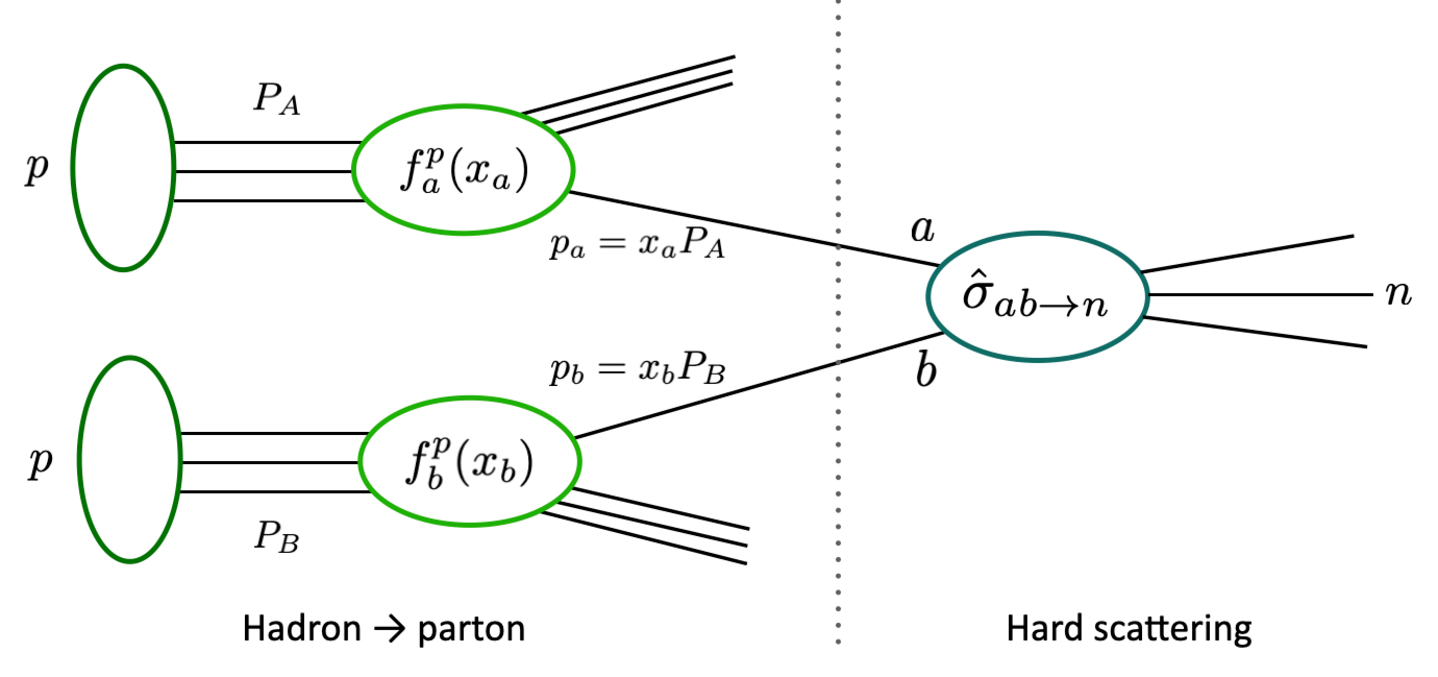
\includegraphics[width=0.8\textwidth,keepaspectratio]{figures/factorization}
%}
\caption{
 factorization theorem 
}
\label{fig:factorization}
\end{center}
\end{figure}

In the scattering process ab$\rightarrow$n at a hadron collider can be written as:
\begin{equation}
\label{eqn:qcdxsec}
\sigma_{a b \rightarrow n}=\sum_{a, b} \int_{0}^{1} \mathrm{~d} x_{a} \mathrm{~d} x_{b} \int \mathrm{d} \Phi_{n} f_{a}^{h_{1}}\left(x_{a}, \mu_{F}\right) f_{b}^{h_{2}}\left(x_{b}, \mu_{F}\right) \times \frac{1}{2 \hat{s}}\left|\mathcal{M}_{a b \rightarrow n}\right|^{2}\left(\Phi_{n} ; \mu_{F}, \mu_{R}\right)
\end{equation}
where a and b is summed over all partonic constituents of the colliding hadrons, $h_1$ and $h_2$, respectively.
$f_{a}^{h_{1}}\left(x_{a}, \mu_{F}\right)$ and $f_{b}^{h_{2}}\left(x_{b}, \mu_{F}\right)$ are the parton distribution function (pdf), obtaining the partons from the original colliding hadrons, at a given momentum fraction x. The factorization depends on the arbitrary cutoff scale, referred as factorization scale, $\mu_F$.
Then the partonic cross section of the hard scattering, $\hat{\sigma}_{a b \rightarrow n}\left(\mu_{F}, \mu_{R}\right)$ can be calculated perturbatively with Feynman-diagrams technique by considering the process $ab\rightarrow n $ with free partons in the initial state. This calculation is done with the Matrix element $\left|\mathcal{M}_{a b \rightarrow n}\right|$ for the phase-space $\Phi_n$.
When calculating the matrix element of the hard-scattering process, the divergence terms are to be absorbed into the redefinition of fields or parameters via subtractions. This procedure is usually referred as renormalization, and the subtractions scale is called renormalization scale, $\mu_R$. 
The PDF is estimated by the collision data from previous and current experiments, and extrapolated to the appropriate energy using the DGLAP evolution equations.\cite{}.
%this reference can be found in "VBS2014"

Since the matrix-element is calculated at a fixed order, final states of parton-level events calculated so far is neglecting higher-order corrections, which have sizable effect on the particle kinematics. In order to account for effects of higher order QCD correction and hadronization, parton showering and hadronization algorithm are performed.

\subsection{Parton shower}
The parton shower do the splittings of the outgoing colored partons.  The MC simulations is base on the Markov-chain, in which the components of the hard subprocess are evolved by adding branchings of one parton into two other partons, in the limit of the infrared cutoff scale, t$_{cutoff}$, typically $t_{0} \approx 1 \mathrm{GeV}$. The typical generators: PYTHIA~\cite{SJOSTRAND2008852} and HERWIG~\cite{Gieseke2012} use different choices of t$_{cutoff}$.
The parton shower doesn't affect to the total cross section, since the final state particles emitted to every directions.
\subsection{Hadoronization}
The partons resulted afterparton shower are combined to form hadrons. Hadronization is performed in completely non-pertabative way, based on several models. PYTHIA and HERWIG adopt different phenomenological models: String Model, based on linear confinement of partons and Cluster Model, based on the preconfinement of parton showers.
%\subsection{MC generators}
%description of MC generators, up to where and what they do



\section{Vector Boson Scattering}
The scattering of two electroweak gauge bosons can probe the structure of the electroweak symmetry breaking (EWSM) mechanism directly. 
Electroweak gauge boson scattering, or Vector Boson Scattering (VBS) is therefore one of the key process to be investigate in LHC experiment.
The Vector Boson indicates W,Z,$\gamma$ here, which are fundamental electroweak bosons. Though the massive vector bosons, which are W and Z are only sensitive to the mechanism of the  EWSM, $\gamma$ is also included since it is impossible to fully separate the $\gamma$ and Z contributions experimentally. 
%<- need this??
\subsection{Electroweak gauge boson scattering and the Higgs boson}
As described in Chapter~\ref{ch:Lagrangian}, the spontaneously symmetry breaking of the local gauge invariance produces three degrees of freedom, which is the GoldStone Bosons and then they are eaten up by the introducing of the Higgs boson. They correspond to the longitudinal, massive weak gauge bosons. Measuring the VBS channels provides information of the other three degrees of freedom than Higgs field. The typical Feynman diagram of VBS is shown in Figure~\ref{fig:VBS}.
%%Correct explanation here????

\begin{figure}[tbp]
\begin{center}
%\subfigure[]{
 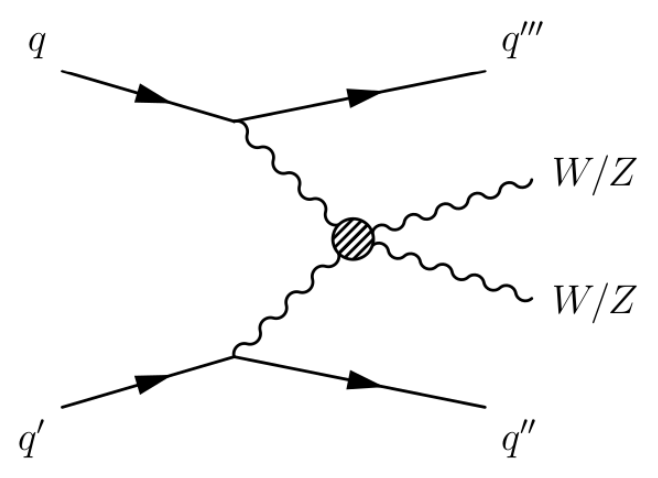
\includegraphics[width=0.50\textwidth,keepaspectratio]{figures/VBS}
%}
\caption{
The Feynman diagram of the VBS. The circle includes any connected diagrams with the external lines at leading order.%, as shown in the Figure\ref{}.
}
\label{fig:VBS}
\end{center}
\end{figure}

\begin{figure}[tbp]
\begin{center}
\subfigure{
 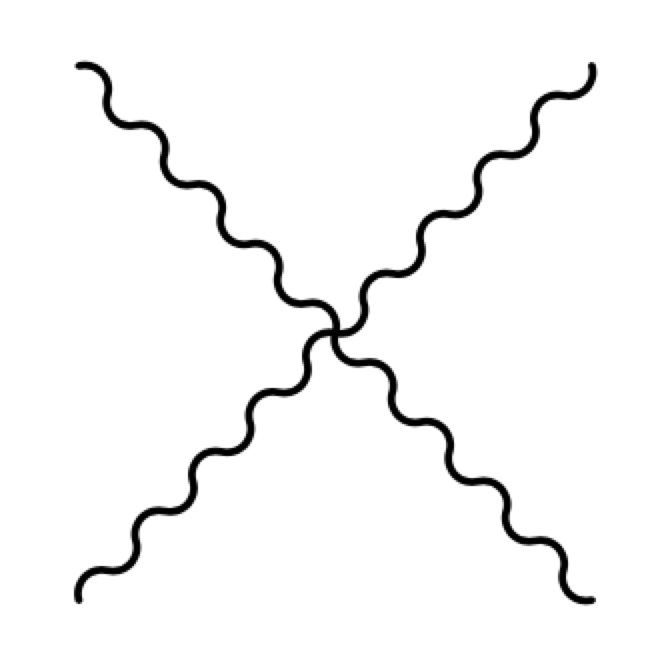
\includegraphics[width=0.20\textwidth,keepaspectratio]{figures/VBS1}
}
\subfigure{
 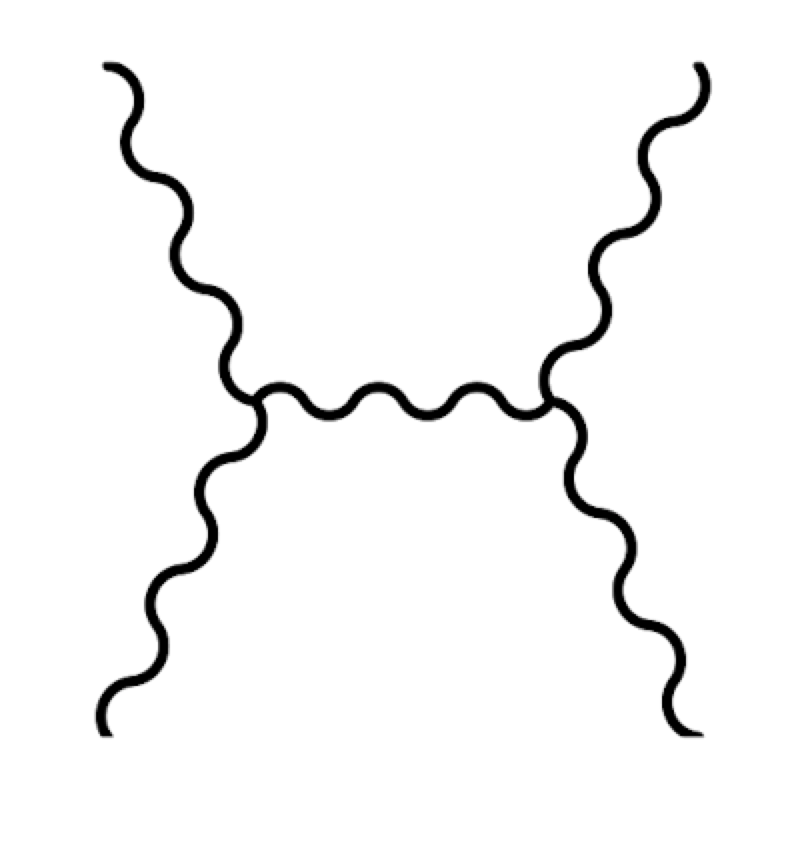
\includegraphics[width=0.19\textwidth,keepaspectratio]{figures/VBS2}
}
\subfigure{
 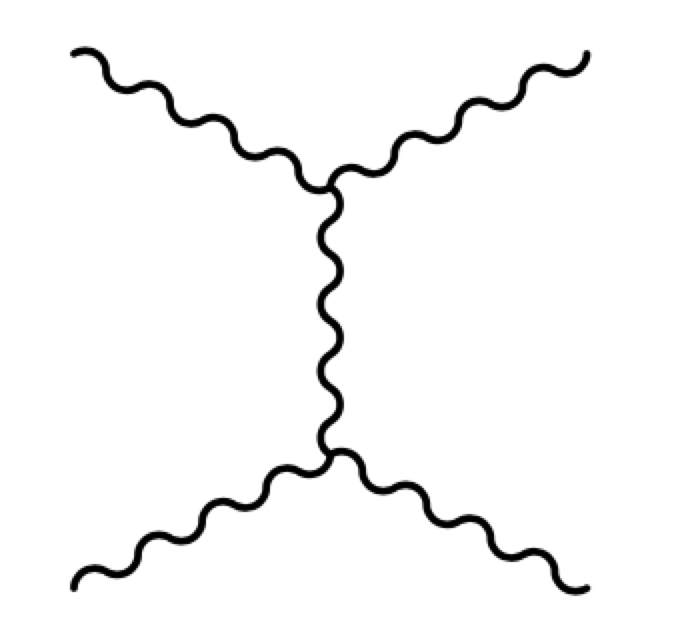
\includegraphics[width=0.21\textwidth,keepaspectratio]{figures/VBS3}
}
\subfigure{
 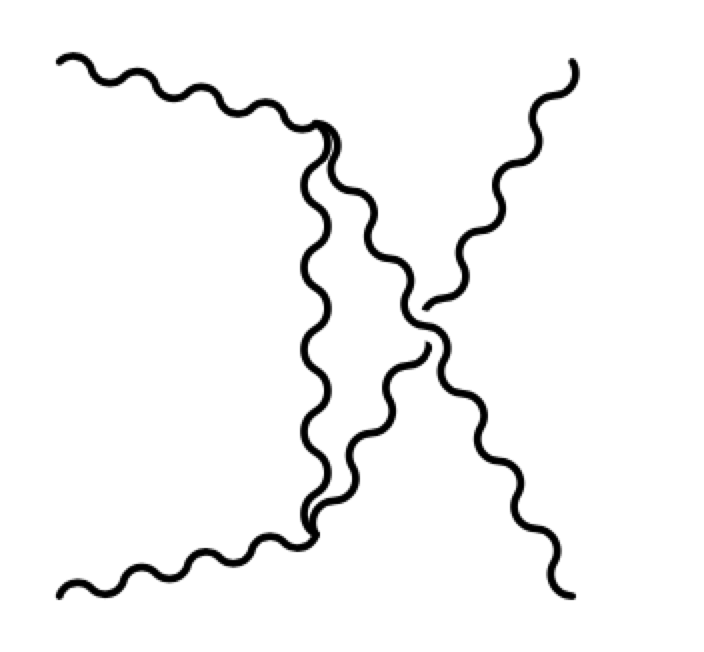
\includegraphics[width=0.21\textwidth,keepaspectratio]{figures/VBS4}
}
\caption{
The VV to VV interaction Feynman diagram at tree-level. Contributions from EW gauge boson interactions.
}
\label{fig:VBSEW}
\end{center}
\end{figure}

\begin{figure}[tbp]
\begin{center}
\subfigure{
 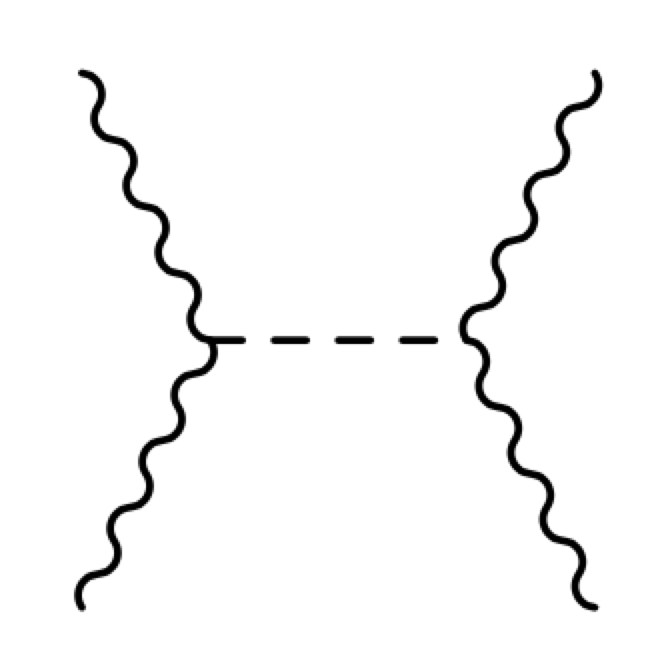
\includegraphics[width=0.20\textwidth,keepaspectratio]{figures/wHiggs1}
}
\subfigure{
 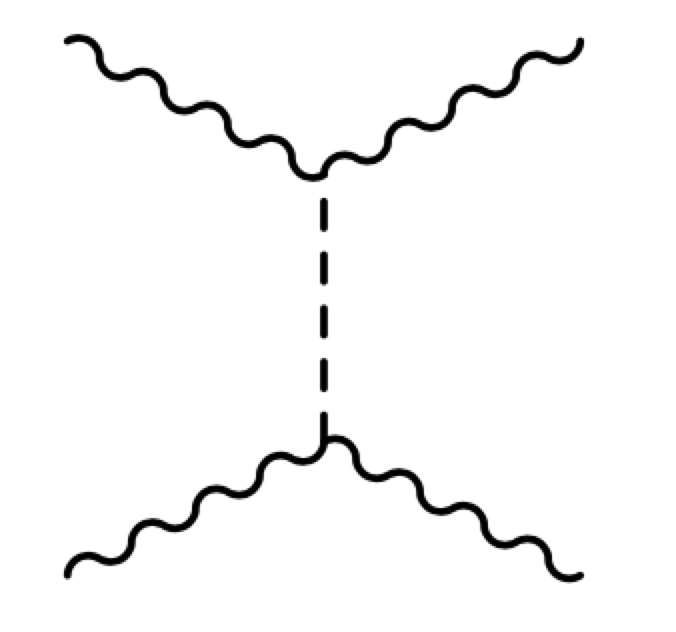
\includegraphics[width=0.20\textwidth,keepaspectratio]{figures/wHiggs2}
}
\subfigure{
 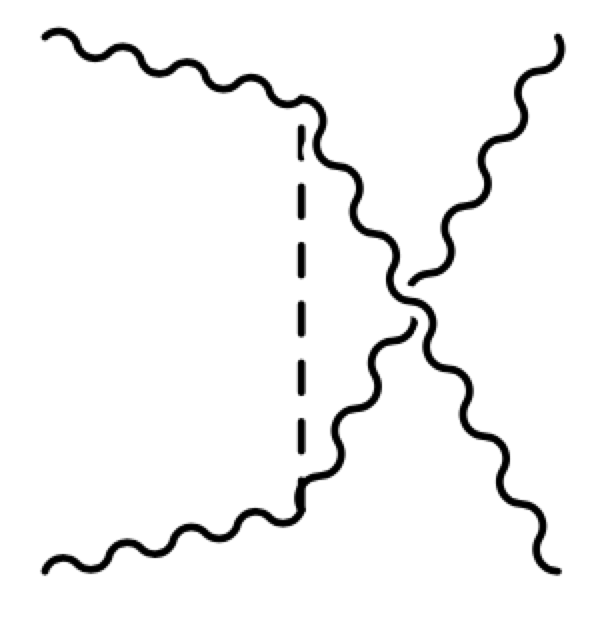
\includegraphics[width=0.18\textwidth,keepaspectratio]{figures/wHiggs3}
}
\caption{
The VV to VV interaction Feynman diagram at tree-level. Contributions includes Higgs boson interactions.
}
\label{fig:VBSHiggs}
\end{center}
\end{figure}


The amplitude of the WW scattering is to be inspected further to see the effect of existence of the Higgs boson for example. The combination of other weak massive bosons like WZ, as well as ZZ can be denoted similarly. 
%really?

Since the polarization vector of the longitudinal weak vector boson can be written in the form, \ref{}: %put reference!
\begin{equation}
\epsilon_{L}^{\mu}=\frac{1}{m_{V}}\left(|\vec{p}|, \frac{\vec{p}}{|\vec{p}|} E\right)=\frac{p^{\mu}}{m_{V}}+\mathcal{O}\left(\frac{m_{V}}{E}\right)
\end{equation}
as the pT glows, the yields with massive vector particles in the initial and finals states will be longitudinal-dominant.
At high-energy limit, the amplitude for $W_L^+W_L^-$ without existing of the Higgs boson (Figure\ref{fig:VBSEW}) can be describes in the form of:
\begin{equation}
\mathcal{M}^{\text {gauge}}=-\frac{g_{w}^{2}}{4 m_{W}^{2}} u+\mathcal{O}\left(\left[\frac{E}{m_{W}}\right]^{0}\right)
\end{equation}
The remaining amplitude from the second term will rise with energy then it violates the unitarity at the unitarity bound. The amplitude including the Higgs contributions (Figure\ref{fig:VBSHiggs}) is:
\begin{equation}
\begin{aligned}
\mathcal{M}^{\text {Higgs}} &=-\frac{g^{2}}{4 m_{W}^{2}}\left[\frac{\left(s-m_{W}^{2}\right)^{2}}{s-m_{H}^{2}}+\frac{\left(t-m_{W}^{2}\right)^{2}}{t-m_{H}^{2}}\right] \\
& \approx \frac{g^{2}}{4 m_{W}^{2}} u,
\end{aligned}
\end{equation}
in the high-energy limit s >> $m_{H}^{2}$, $m_{W}^{2}$.
Therefore the terms affected by the rising energy cancel and leave the constant term, which is not violating the unitarity.
%The energy scale where the unitarity is violated

This effect also described with the Figure~\ref{fig:violation}.
The figure shows that if diagrams with Higgs contribution is missing, the electroweak couplings becomes strong around $\sqrt{s}$ ∼ 1 TeV, and the unitarity of the $W_LW_L \rightarrow W_LW_L$ process is violated, which means the SM without the Higgs boson is no longer valid above TeV-scale. 

\begin{figure}[tbp]
\begin{center}
%\subfigure[]{
 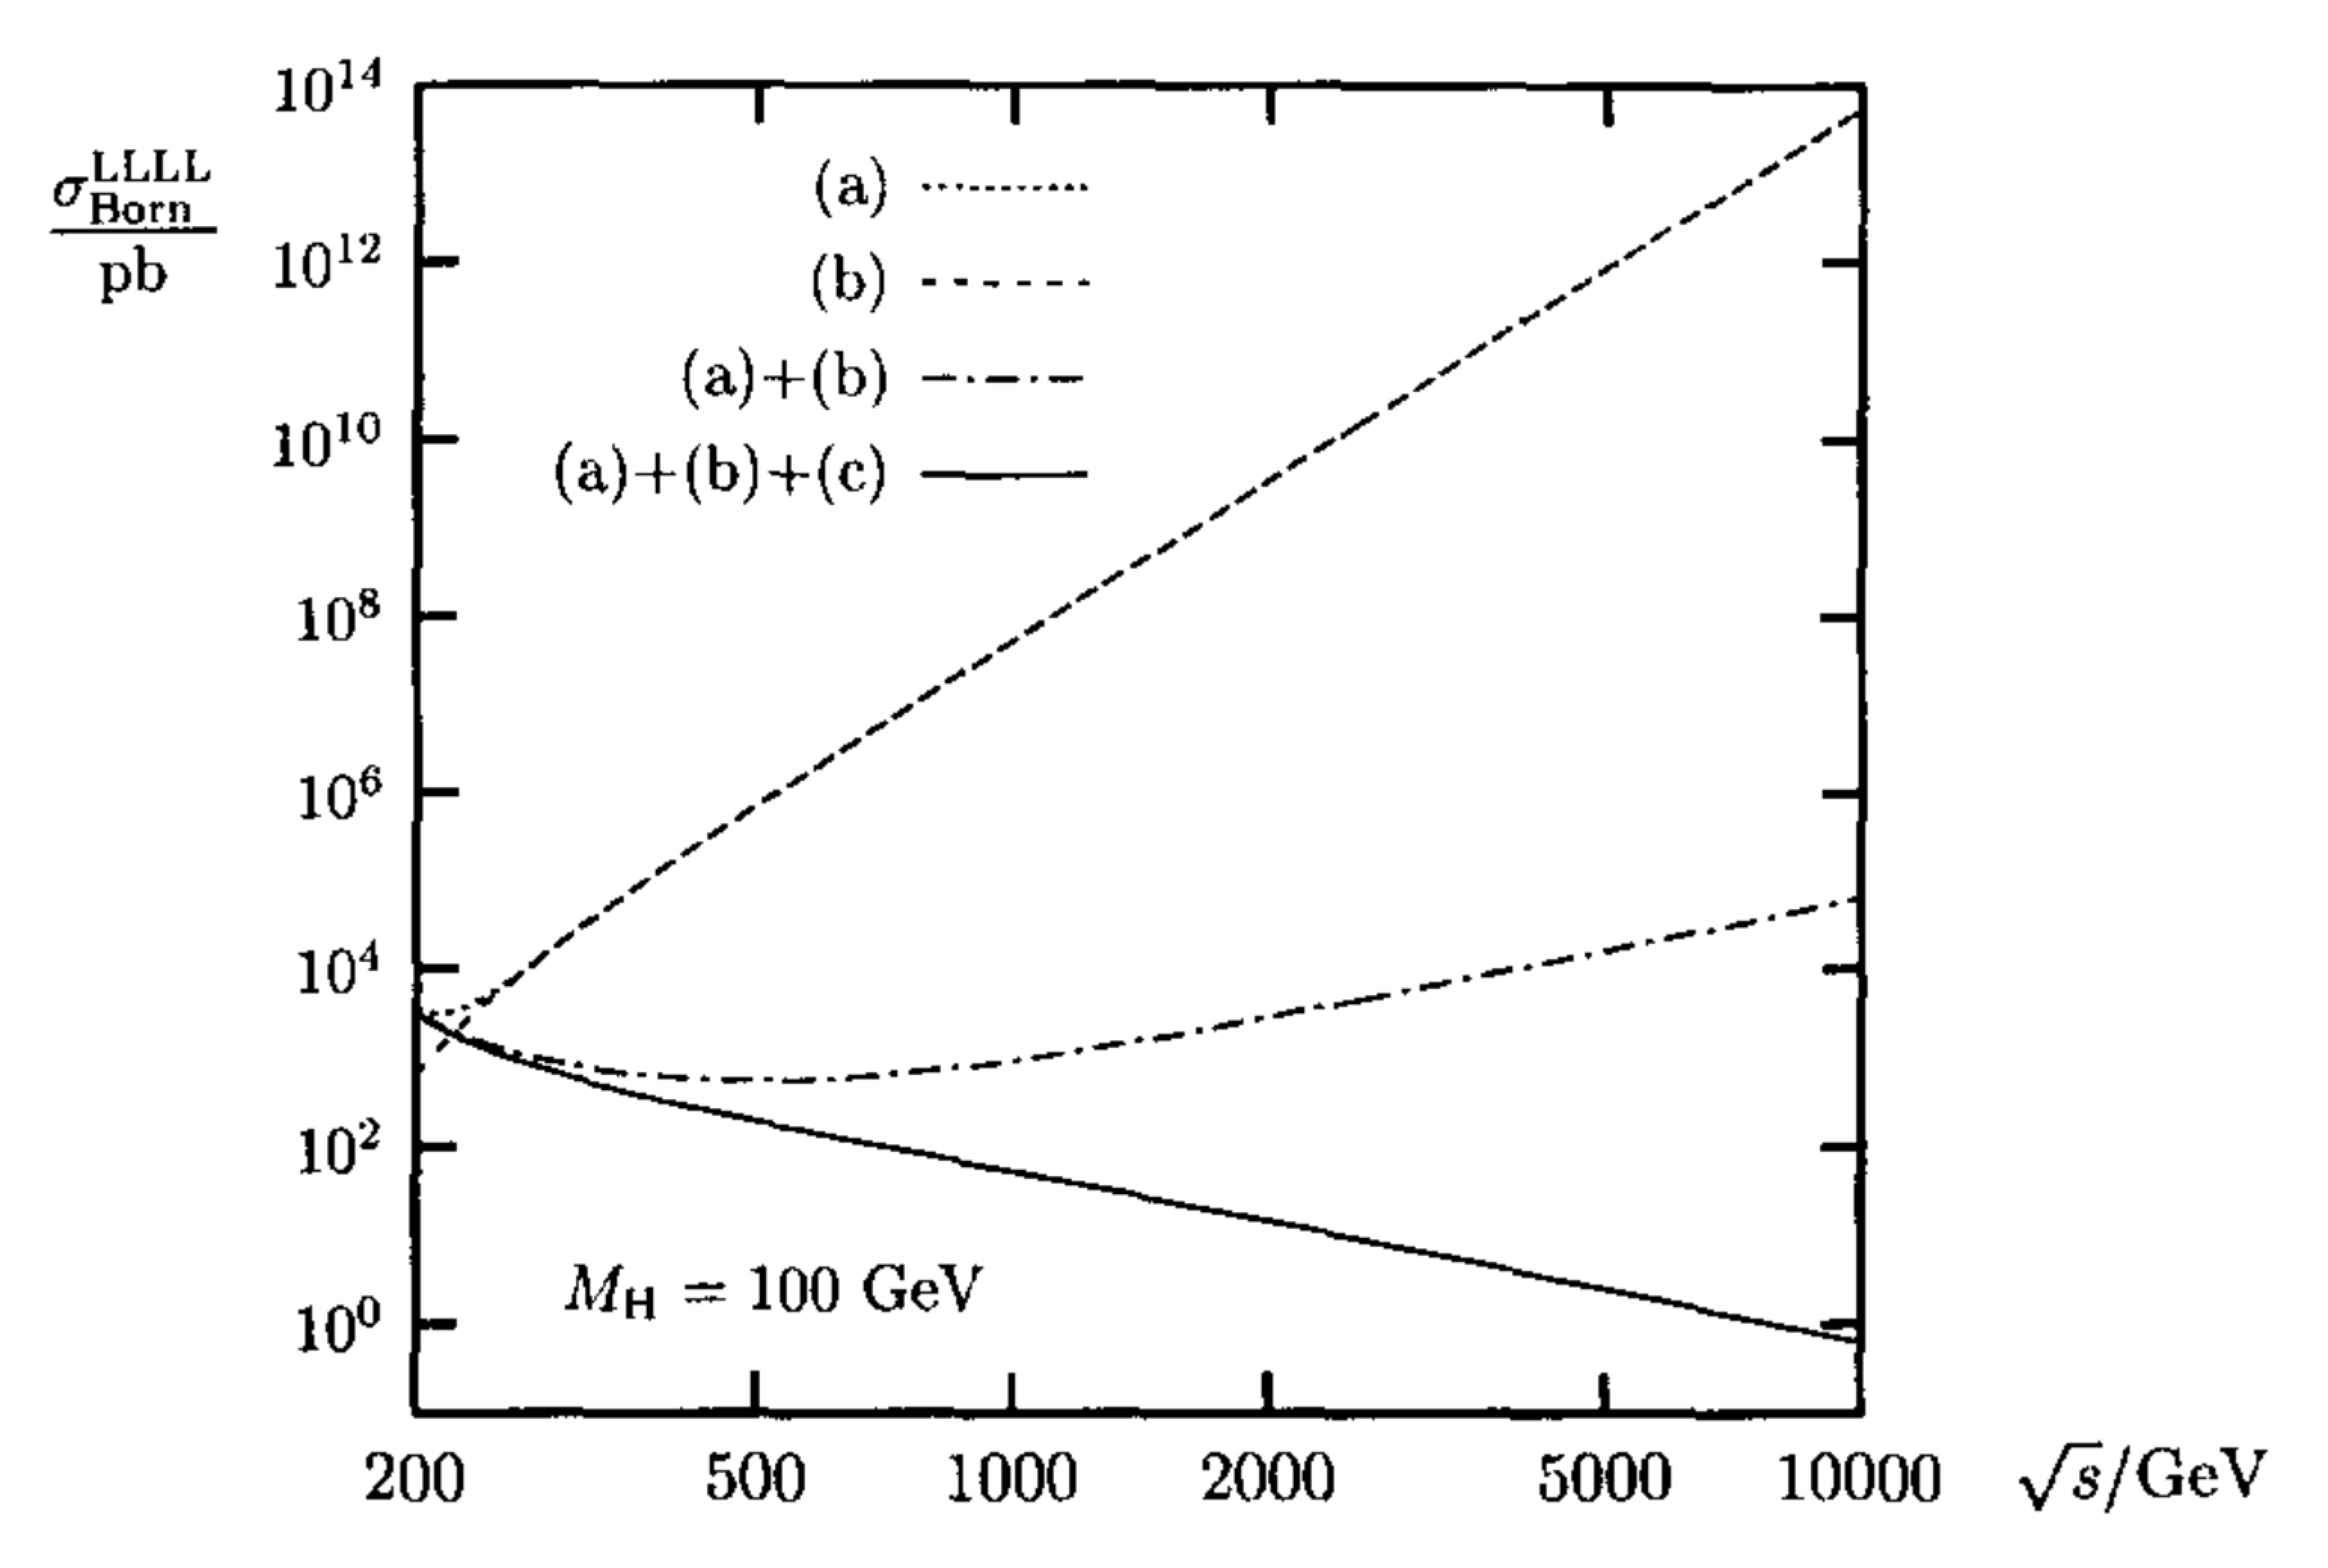
\includegraphics[width=0.80\textwidth,keepaspectratio]{figures/violation}
%}
\caption{
Cross section at tree-level %\ref{}
}
\label{fig:violation}
\end{center}
\end{figure}

\section{Production Cross-Sections and Branching Fractions}
\\
\\

\section{Anomalous Quartic Gauge Coupling and Effective Field Theory}

\subsection{aQGC}
The unitarity recovered by the existence of Higgs boson can be broken again by the additional quartic gauge coupling by new physics. This is referred to as anomalous quartic gauge couplings (aQGC). 

\subsection{EFT}
Since the aQGC can claim many different models, The Effective Field Theory (EFT) is considered as a model-independent way of the interpretation. The EFT models the effects of new physics at energy scale much higher than the currently accessible range by the experiments. The SM is regarded as an effective theory at low-energy in this framework.The EFT contains additional operators with higher energy dimension suppressed by the cutoff scale of the new physics, $\Lambda$.
The EFT Lagrangian is given as:
\begin{equation}
\mathcal{L}_{\mathrm{EFT}}=\mathcal{L}_{\mathrm{SM}}+\sum_{d>4} \sum_{i} \frac{c_{i}^{(d)}}{\Lambda^{d-4}} \mathcal{O}_{i}^{(d)}
\end{equation}
where $c_{i}^{(d)}$ are the Wilson coefficients of the new operators, $\mathcal{O}_{i}^{(d)}$.
$\Lambda$ is a cutoff scale, and the d is a mass dimensions which fulfill d > 4.
Any new physics can be modeled in this framework by certain additional operators, where their coefficient is also fixed as long as the new physics scale is above the cutoff scale, $\Lambda$. The SM is a low-energy theory in this framework, i.e. if $\Lambda \rightarrow \infty$, the SM is reproduced.
\\

To model possible aQGC effect in the VBS process, the Eboli model \cite{eboli2006p} which introduces new dimension 8 operators which satisfy the SM $SU(2)\times U(1)_Y$ symmetry are used. 

The lowest dimension operator that leads to quartic interactions and does not exhibit two or three weak gauge boson vertices is dimension 8. 
This is when we get a weak boson field either from the covariant derivative of Higgs doublet $\Phi$ or from the field strength tensor. 
In either case the vector field is accompanied by a vacuum expected value or a derivative, therefore the genuine quartic vertices are of dimension 8 or higher.
%understand this?
All the corresponding operators are shown hereafter.

\begin{itemize}
\item Operators containing just $D_\mu \Phi$
\begin{equation}
\begin{aligned}
\mathcal{L}_{S, 0} &=\left[\left(D_{\mu} \Phi\right)^{\dagger} D_{\nu} \Phi\right] \times\left[\left(D^{\mu} \Phi\right)^{\dagger} D^{\nu} \Phi\right] \\
\mathcal{L}_{S, 1} &=\left[\left(D_{\mu} \Phi\right)^{\dagger} D^{\mu} \Phi\right] \times\left[\left(D_{\nu} \Phi\right)^{\dagger} D^{\nu} \Phi\right] \\
\mathcal{L}_{S, 2} &=\left[\left(D_{\mu} \Phi\right)^{\dagger} D_{\nu} \Phi\right] \times\left[\left(D^{\nu} \Phi\right)^{\dagger} D^{\mu} \Phi\right]
\end{aligned}
\end{equation}
\item Operators containing $D_\mu \Phi$ and field strength 
\begin{equation}
\begin{aligned}
\mathcal{L}_{M, 0} &=\operatorname{Tr}\left[\hat{W}_{\mu \nu} \hat{W}^{\mu \nu}\right] \times\left[\left(D_{\beta} \Phi\right)^{\dagger} D^{\beta} \Phi\right] \\
\mathcal{L}_{M, 1} &=\operatorname{Tr}\left[\hat{W}_{\mu \nu} \hat{W}^{\nu \beta}\right] \times\left[\left(D_{\beta} \Phi\right)^{\dagger} D^{\mu} \Phi\right] \\
\mathcal{L}_{M, 2} &=\left[B_{\mu \nu} B^{\mu \nu}\right] \times\left[\left(D_{\beta} \Phi\right)^{\dagger} D^{\beta} \Phi\right] \\
\mathcal{L}_{M, 3} &=\left[B_{\mu \nu} B^{\nu \beta}\right] \times\left[\left(D_{\beta} \Phi\right)^{\dagger} D^{\mu} \Phi\right] \\
\mathcal{L}_{M, 4} &=\left[\left(D_{\mu} \Phi\right)^{\dagger} \hat{W}_{\beta \nu} D^{\mu} \Phi\right] \times B^{\beta \nu} \\
\mathcal{L}_{M, 5} &=\left[\left(D_{\mu} \Phi\right)^{\dagger} \hat{W}_{\beta \nu} D^{\nu} \Phi\right] \times B^{\beta \mu} \\
\mathcal{L}_{M, 6} &=\left[\left(D_{\mu} \Phi\right)^{\dagger} \hat{W}_{\beta \nu} \hat{W}^{\beta \nu} D^{\mu} \Phi\right] \\
\mathcal{L}_{M, 7} &=\left[\left(D_{\mu} \Phi\right)^{\dagger} \hat{W}_{\beta \nu} \hat{W}^{\beta \mu} D^{\nu} \Phi\right]
\end{aligned}
\end{equation}
\item Operators containing just the field strength tensor
\begin{equation}
\begin{aligned}
\mathcal{L}_{T, 0} &=\operatorname{Tr}\left[\hat{W}_{\mu \nu} \hat{W}^{\mu \nu}\right] \times \operatorname{Tr}\left[\hat{W}_{\alpha \beta} \hat{W}^{\alpha \beta}\right] \\
\mathcal{L}_{T, 1} &=\operatorname{Tr}\left[\hat{W}_{\alpha \nu} \hat{W}^{\mu \beta}\right] \times \operatorname{Tr}\left[\hat{W}_{\mu \beta} \hat{W}^{\alpha \nu}\right] \\
\mathcal{L}_{T, 2} &=\operatorname{Tr}\left[\hat{W}_{\alpha \mu} \hat{W}^{\mu \beta}\right] \times \operatorname{Tr}\left[\hat{W}_{\beta \nu} \hat{W}^{\nu \alpha}\right] \\
\mathcal{L}_{T, 3} &=\operatorname{Tr}\left[\hat{W}_{\alpha \mu} \hat{W}^{\mu \beta} \hat{W}^{\nu \alpha}\right] \times B_{\beta \nu} \\
\mathcal{L}_{T, 4} &=\operatorname{Tr}\left[\hat{W}_{\alpha \mu} \hat{W}^{\alpha \mu} \hat{W}^{\beta \nu}\right] \times B_{\beta \nu} \\
\mathcal{L}_{T, 5} &=\operatorname{Tr}\left[\hat{W}_{\mu \nu} \hat{W}^{\mu \nu}\right] \times B_{\alpha \beta} B^{\alpha \beta} \\
\mathcal{L}_{T, 6} &=\operatorname{Tr}\left[\hat{W}_{\alpha \nu} \hat{W}^{\mu \beta}\right] \times B_{\mu \beta} B^{\alpha \nu} \\
\mathcal{L}_{T, 7} &=\operatorname{Tr}\left[\hat{W}_{\alpha \mu} \hat{W}^{\mu \beta}\right] \times B_{\beta \nu} B^{\nu \alpha} \\
\mathcal{L}_{T, 8} &=B_{\mu \nu} B^{\mu \nu} B_{\alpha \beta} B^{\alpha \beta} \\
\mathcal{L}_{T, 9} &=B_{\alpha \mu} B^{\mu \beta} B_{\beta \nu} B^{\nu \alpha}
\end{aligned}
\end{equation}
\end{itemize}

Since the operator $\mathcal{L}_{S, 2}$ is the Hermite conjugate of the $\mathcal{L}_{S, 0}$, those 2 operators are treated as single operator denoted as $\mathcal{L}_{S, 02}$, with the coefficient $f_S02$, respectively. It is found via simulations that the tensor operators produce purely transversely polarized $W/Z$ bosons, while the scalar operators longitudinal bosons.

The summary of the correspondences of the operators and the vertices are summarized in the table~\ref{tab:vertex}.

%table1
\begin{center}
\begin{tabular}{|l| c c c c c c c c c|} 
 \hline
 operators                                                & $WWWW$ & $WWZZ$ & $ZZZZ$ & $WW\gamma Z$ & $WW\gamma \gamma$ & $ZZZ\gamma$ & $ZZ\gamma \gamma$ & $Z\gamma \gamma \gamma$ & $\gamma \gamma \gamma \gamma \gamma$\\ [0.5ex] 
 \hline\hline
 $\mathcal{L}_{S02}$,$\mathcal{L}_{S1}$                   & \checkmark & \checkmark & \checkmark &  &  &  &  & & \\ 
 \hline
 $\mathcal{L}_{M0}$,$\mathcal{L}_{M1}$,$\mathcal{L}_{M7}$ & \checkmark & \checkmark & \checkmark & \checkmark & \checkmark &\checkmark &\checkmark & &\\
 \hline
 $\mathcal{L}_{M2}$,$\mathcal{L}_{M3}$,$\mathcal{L}_{M4}$,$\mathcal{L}_{M5}$ &  & \checkmark & \checkmark & \checkmark & \checkmark & \checkmark &\checkmark & &\\
 \hline
 $\mathcal{L}_{T0}$,$\mathcal{L}_{T1}$,$\mathcal{L}_{T2}$ &  & \checkmark & \checkmark & \checkmark & \checkmark & \checkmark & \checkmark & &\\
 \hline
 $\mathcal{L}_{T5}$,$\mathcal{L}_{T6}$,$\mathcal{L}_{T7}$ & \checkmark & \checkmark & \checkmark & \checkmark & \checkmark & \checkmark &\checkmark &\checkmark &\checkmark\\ [1ex] 
 \hline
 $\mathcal{L}_{T8}$,$\mathcal{L}_{T9}$                    &  &  & \checkmark &  &  & \checkmark &\checkmark &\checkmark &\checkmark\\ [1ex] 
 \hline
\end{tabular}
\caption{operators and the vertices}
\label{tab:vertex}
\end{center}

The aQGCs can be measured by the VBS and the triboson channels.
The summary of sensitive channel to each operator is shown in the table~\ref{tab:aQGCchannel}. \textcolor{blue}{need to think and modify this table}

%table2
\begin{center}
\begin{tabular}{|l| c c c c c c |} 
 \hline
 VVjj final state                                         & $ZZ$ & $WWZZ$ & $ZZZZ$ & $WW\gamma Z$ & $WW\gamma \gamma$ & $ZZZ\gamma$ \\ [0.5ex] 
 \hline\hline
 VVV final state                                          & $ZZZ$ & $WWZZ$ & $ZZZZ$ & $WW\gamma Z$ & $WW\gamma \gamma$ & $ZZZ\gamma$ \\ [0.5ex] 
 \hline\hline
 $\mathcal{L}_{S02}$,$\mathcal{L}_{S1}$                   & \checkmark & \checkmark & \checkmark &  &           &  \\ 
 \hline
 $\mathcal{L}_{M0}$,$\mathcal{L}_{M1}$,$\mathcal{L}_{M7}$ & \checkmark & \checkmark & \checkmark & \checkmark & \checkmark &\checkmark \\
 \hline
 $\mathcal{L}_{M2}$,$\mathcal{L}_{M3}$,$\mathcal{L}_{M4}$,$\mathcal{L}_{M5}$ &  & \checkmark & \checkmark & \checkmark & \checkmark & \checkmark\\
 \hline
 $\mathcal{L}_{T0}$,$\mathcal{L}_{T1}$,$\mathcal{L}_{T2}$ &  & \checkmark & \checkmark & \checkmark & \checkmark & \checkmark \\
 \hline
 $\mathcal{L}_{T5}$,$\mathcal{L}_{T6}$,$\mathcal{L}_{T7}$ & \checkmark & \checkmark & \checkmark & \checkmark & \checkmark & \checkmark \\ [1ex] 
 \hline
 $\mathcal{L}_{T8}$,$\mathcal{L}_{T9}$                    &  &  & \checkmark &  &  & \checkmark \\ [1ex] 
 \hline
\end{tabular}
\caption{operators and the channels}
\label{tab:aQGCchannel}
\end{center}


\chapter{The LHC-ATLAS Experiment}
\section{Large Hadron Collider}
\begin{figure}[tbp]
\begin{center}
%\subfigure[]{
 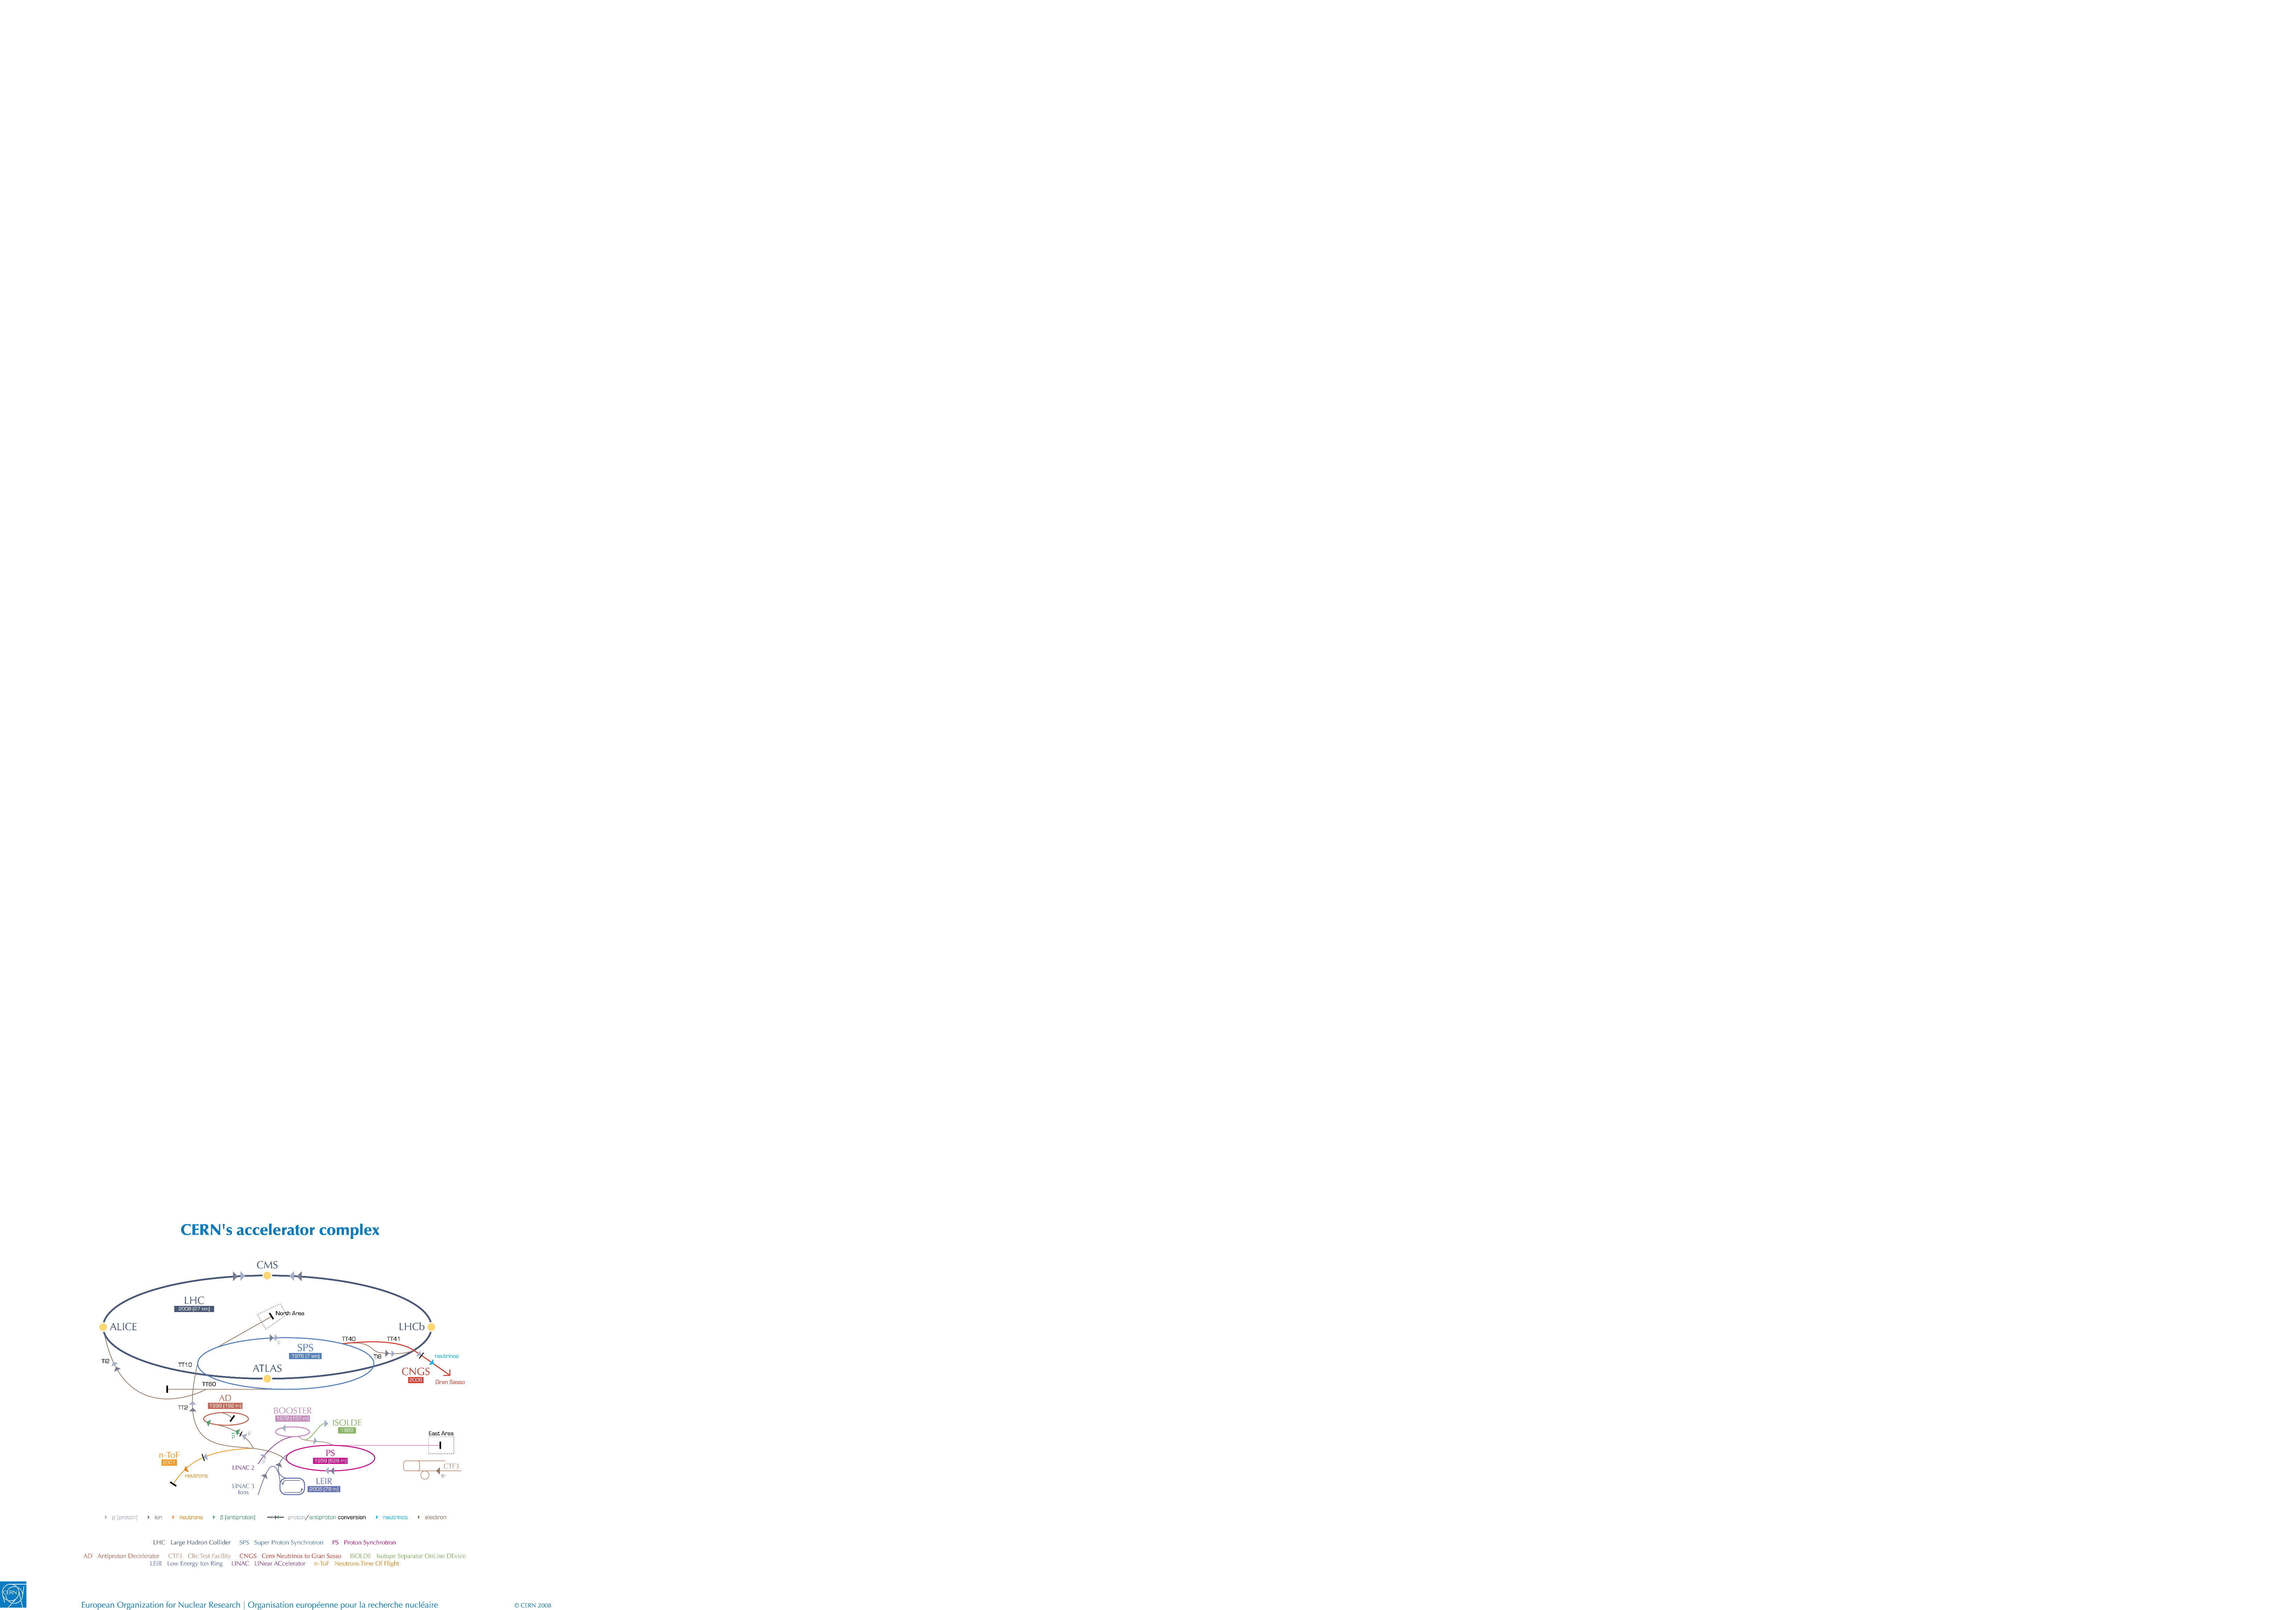
\includegraphics[width=1.0\textwidth,keepaspectratio]{figures/detector/CERN}
%}
\caption{
The whole picture of the CERN accelerator complex
}
\label{fig:CERN}
\end{center}
\end{figure}

\section{ATLAS Detector}
The ATLAS Detector [11] was designed to measure all standard model particles 2) produced by LHC collisions, a schematic overview of the whole ATLAS detector is shown in Figure 3.2. The detector position surrounding the beam pipe called barrel, and those aligned at the high η regions are referred to as end-caps.
The magnet system and the luminosity detector are introduced in Section 3.3.1 and 3.3.2, respectively. Four major subsystems, the inter tracker, the calorimeters, the muon spectrometer, and the trigger & data acquisition system are described.
\begin{figure}[tbp]
\begin{center}
%\subfigure[]{
 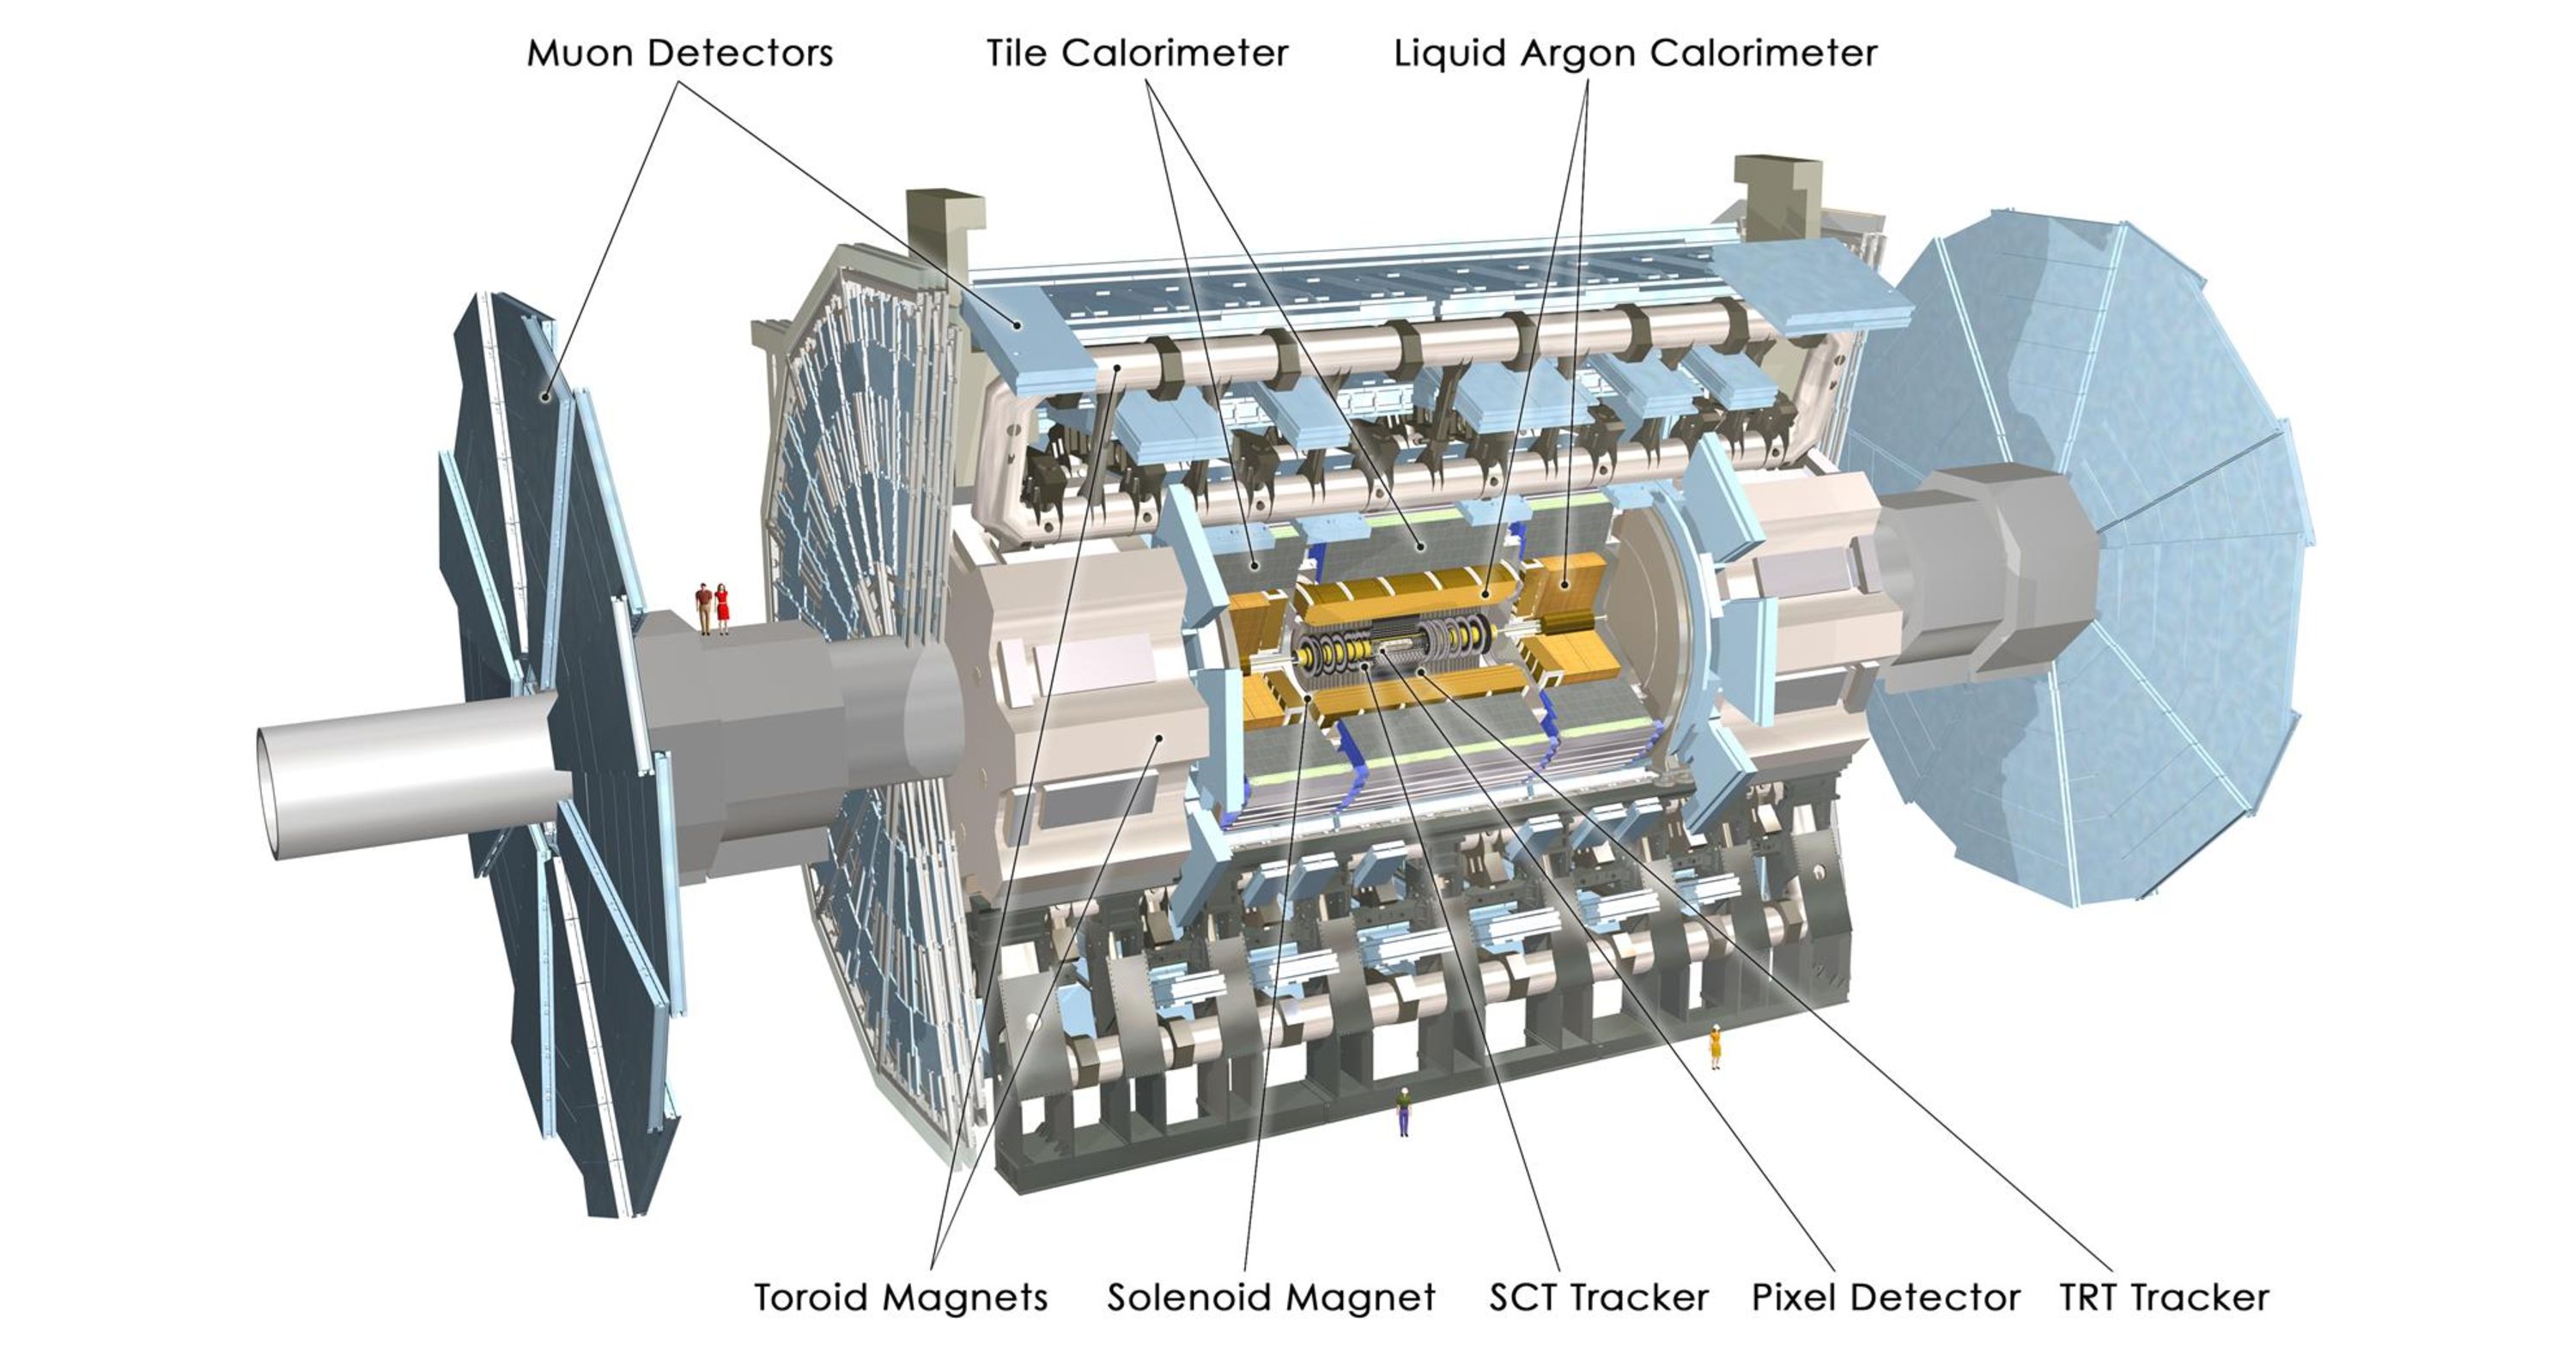
\includegraphics[width=1.0\textwidth,keepaspectratio]{figures/detector/ATLAS}
%}
\caption{
The whole picture of the ATLAS detector
}
\label{fig:CERN}
\end{center}
\end{figure}

\subsection{Magnet}
The ATLAS magnet system consists of four large superconducting magnets with a dimension of 22 m in diameter and 26 m in length with a stored energy of 1.6 GJ. A solenoid aligned on the beam axis generates 2 T axial magnetic field for the inner detector, which placed inside the calorimeter system. A toroid on the barrel and two toroids on the end-caps are installed and those provide 0.5 and 1T magnetic fields for muon detectors, respectively.
\subsection{Inner Tracker}
\subsubsection{Pixel Detector}
\subsubsection{SCT Detector}
\subsubsection{TRT Detector}
\subsection{Calorimeters}
\subsection{Muon Spectrometer}
\subsection{Trigger and Data Aquisition System}
\chapter{Object definition}
\section{Tracks and Vertices}
\section{Clusters}
\section{Electrons}
\section{Muons}
\section{Jets}
\subsection{small-R Jets}
\subsection{large-R Jets}
\section{Missing Transverse Momentum}


\chapter{Signal Optimisation}

\chapter{Multi-Variate Analysis}

In order to improve the separation with respect to the other SM background processes, we use a Machine Learning approach for the analysis. The approach adopted in this analysis is a Recurrent Neural Network (RNN) architecture.

\section{RNN}
\section{Input variables}
\section{Setup and training}
\section{Optimization of the binning}
The optimization of the binning is needed to get the optimal performance of the RNN. The transformation of the RNN output to optimise the effect of the final sensitivity and reduction in the number of bins is implemented.

The Transformation D~\cite{ATL-PHYS-PUB-2019-009} is implemented.
For the current analysis, z$_s$ = 10, z$_b$ = 5 is used for the optimal parameter. In addition, MC statistical uncertainty in each bin is required to be $<$ 20~\% to minimise the bias on fitted $\mu$~\cite{ATL-PHYS-PUB-2019-009}.
\chapter{Background Estimation}

\section{Z+jets modeling}

The Z +jets production is the leading background for the 2-lepton analysis and contributes significantly for the 0-lepton analysis. The comparison of distributions from data and MC for various kinematic variables after re-weighting in the 2-lepton Z+jets merged and resolved control region are shown in Figure \ref{fig:2lep_zjets_merged_CR} and Figure \ref{fig:2lep_zjets_resolved_CR} respectively.

% 2-lepton new merged CR - plots
%\begin{figure}[ht]
%    \centering
%    \subfigure[]{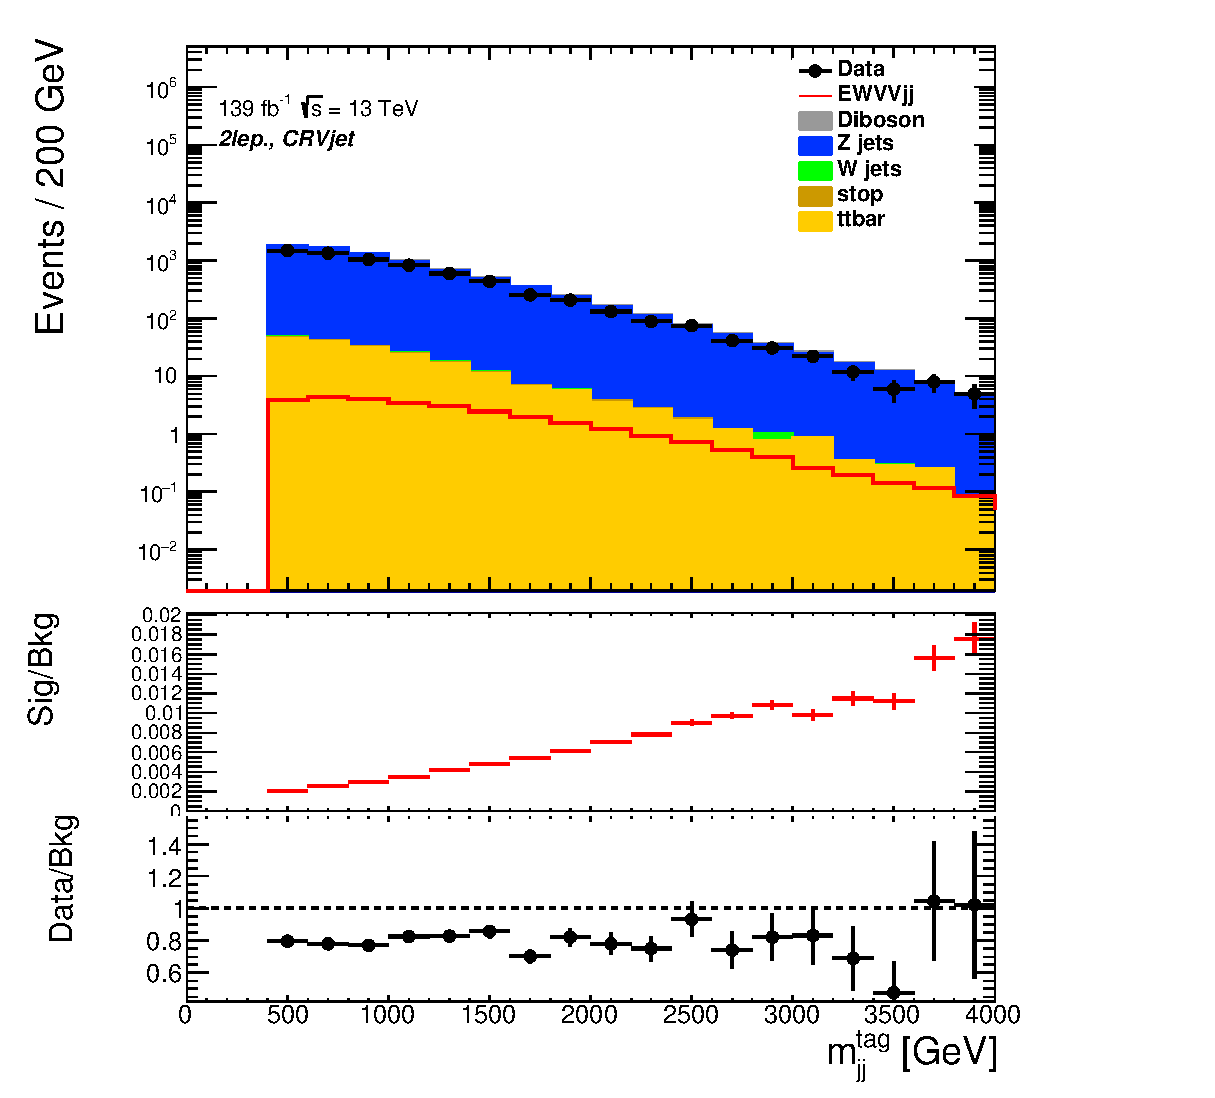
\includegraphics[width=0.45\textwidth]{figures/2lep/reweighting/after_reweighting/C_0ptag1pfat0pjet_0ptv_CRVjet_MTagMerJets_Log.eps}}
%    \subfigure[]{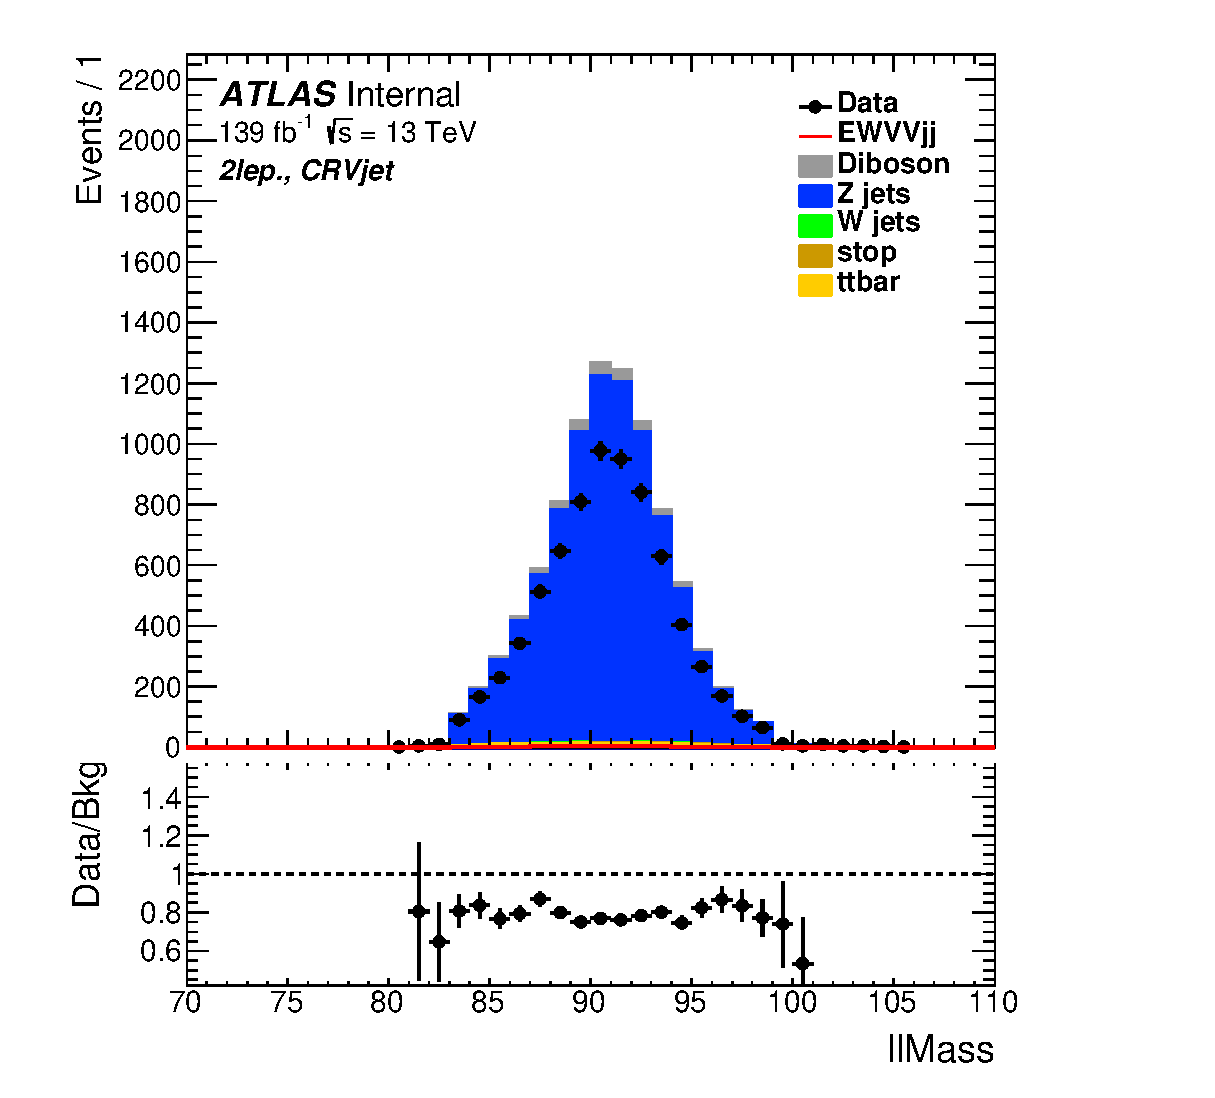
\includegraphics[width=0.45\textwidth]{figures/2lep/reweighting/after_reweighting/C_0ptag1pfat0pjet_0ptv_CRVjet_llMass_Lin.eps}}
%    \subfigure[]{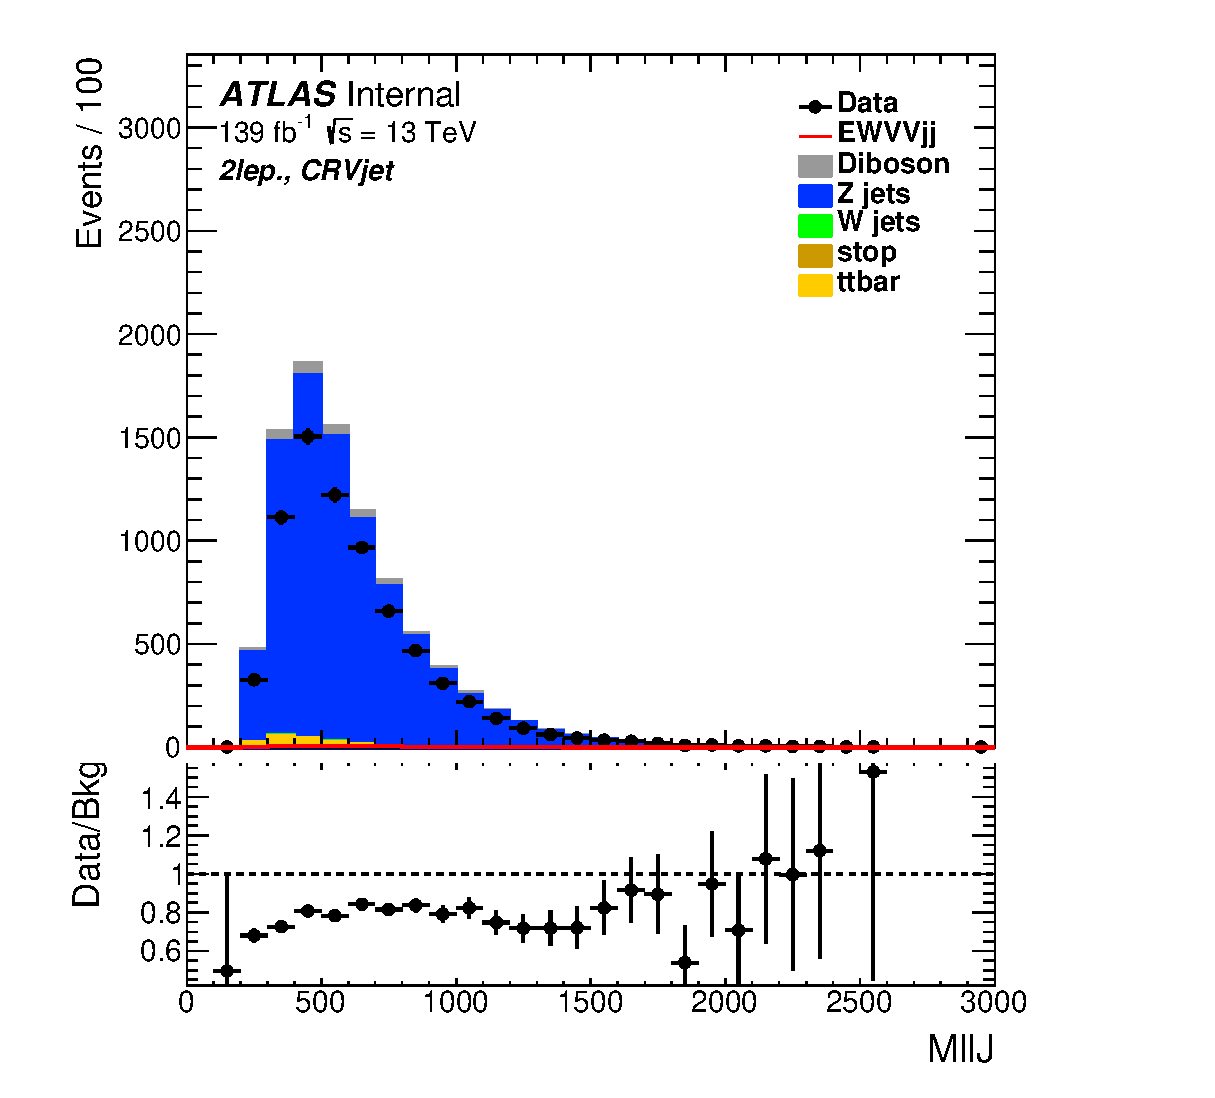
\includegraphics[width=0.45\textwidth]{figures/2lep/reweighting/after_reweighting/C_0ptag1pfat0pjet_0ptv_CRVjet_MllJ_Lin.eps}}
%    \subfigure[]{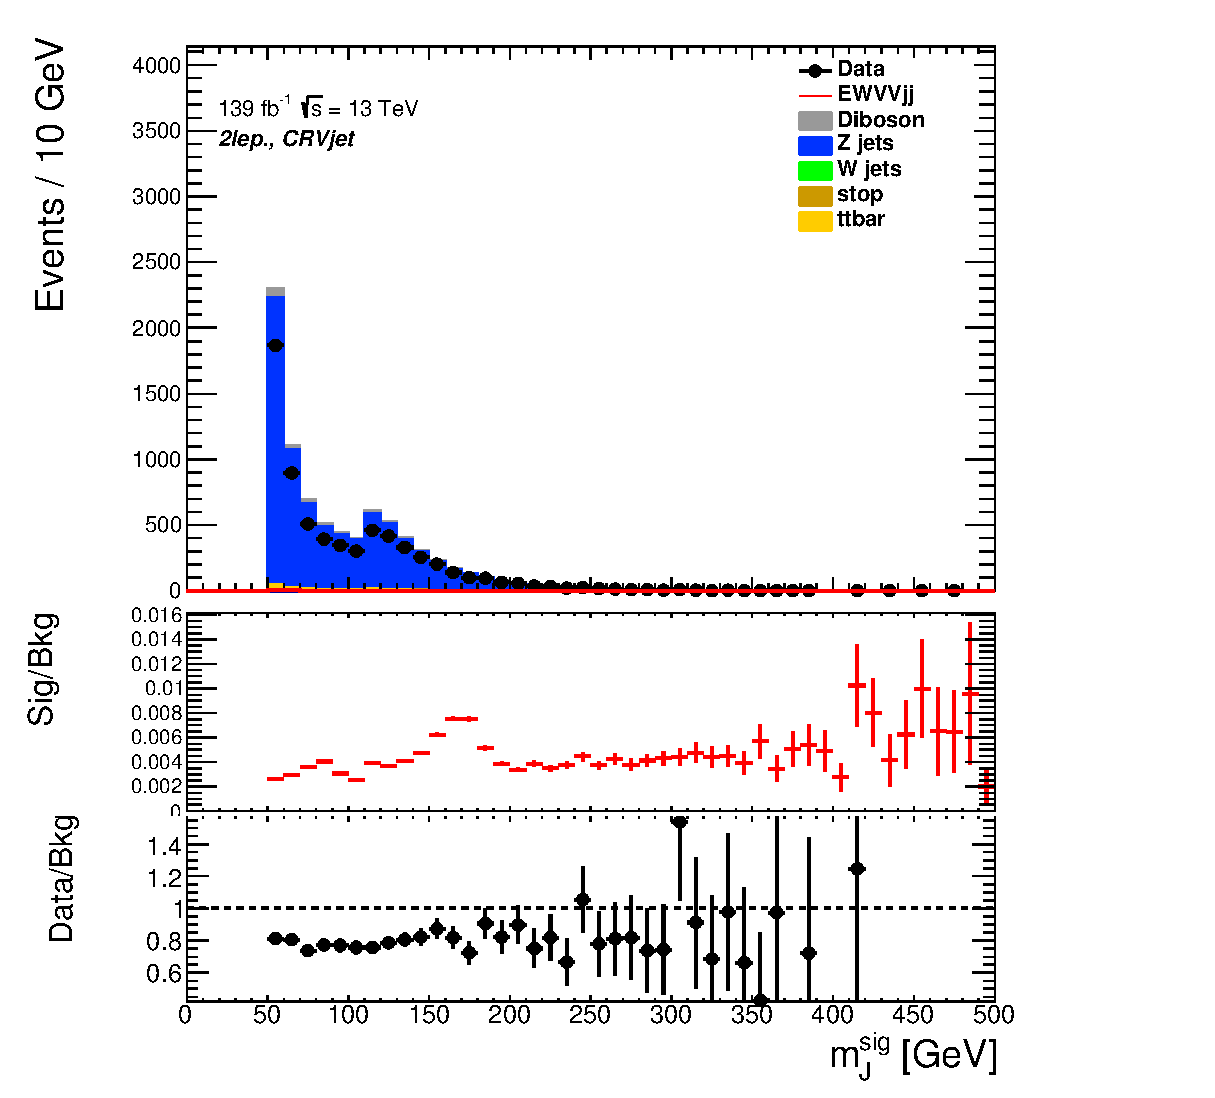
\includegraphics[width=0.45\textwidth]{figures/2lep/reweighting/after_reweighting/C_0ptag1pfat0pjet_0ptv_CRVjet_fatJetMass_Lin.eps}}
%    \caption{ Various kinematic variables in the Z+jets merged CR in the 2-lepton channel analysis.}
%    \label{fig:2lep_zjets_merged_CR}
%\end{figure}


% 2-lepton resolved CR fiducial- plots
%\begin{figure}[ht]
%    \centering
%    \subfigure[]{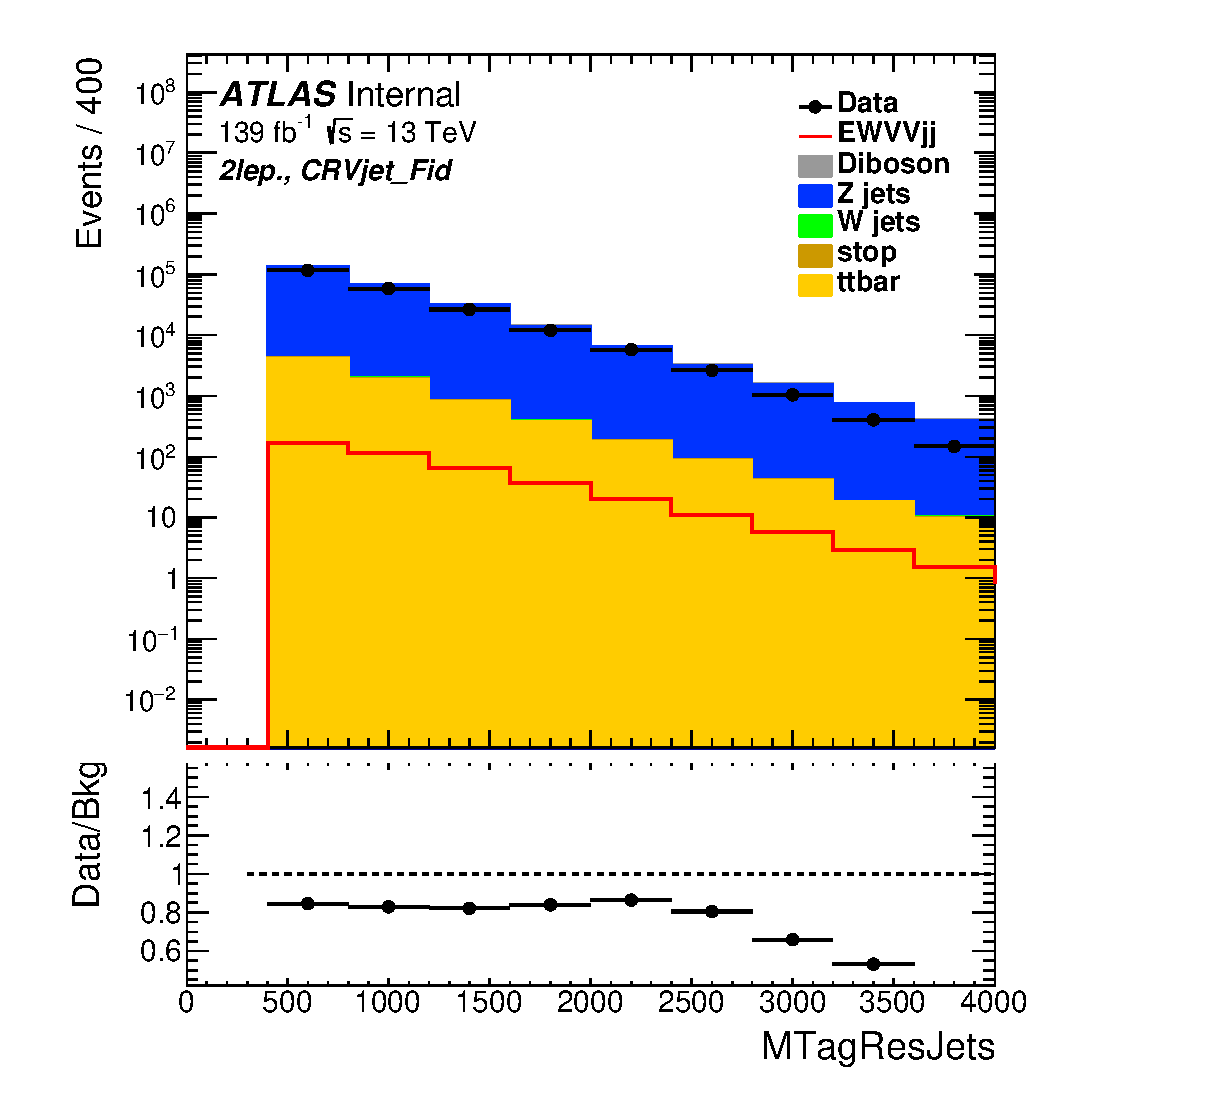
\includegraphics[width=0.45\textwidth]{figures/2lep/reweighting/after_reweighting/C_0ptag2pjet_0ptv_CRVjet_Fid_MTagResJets_Log.eps}}
%    \subfigure[]{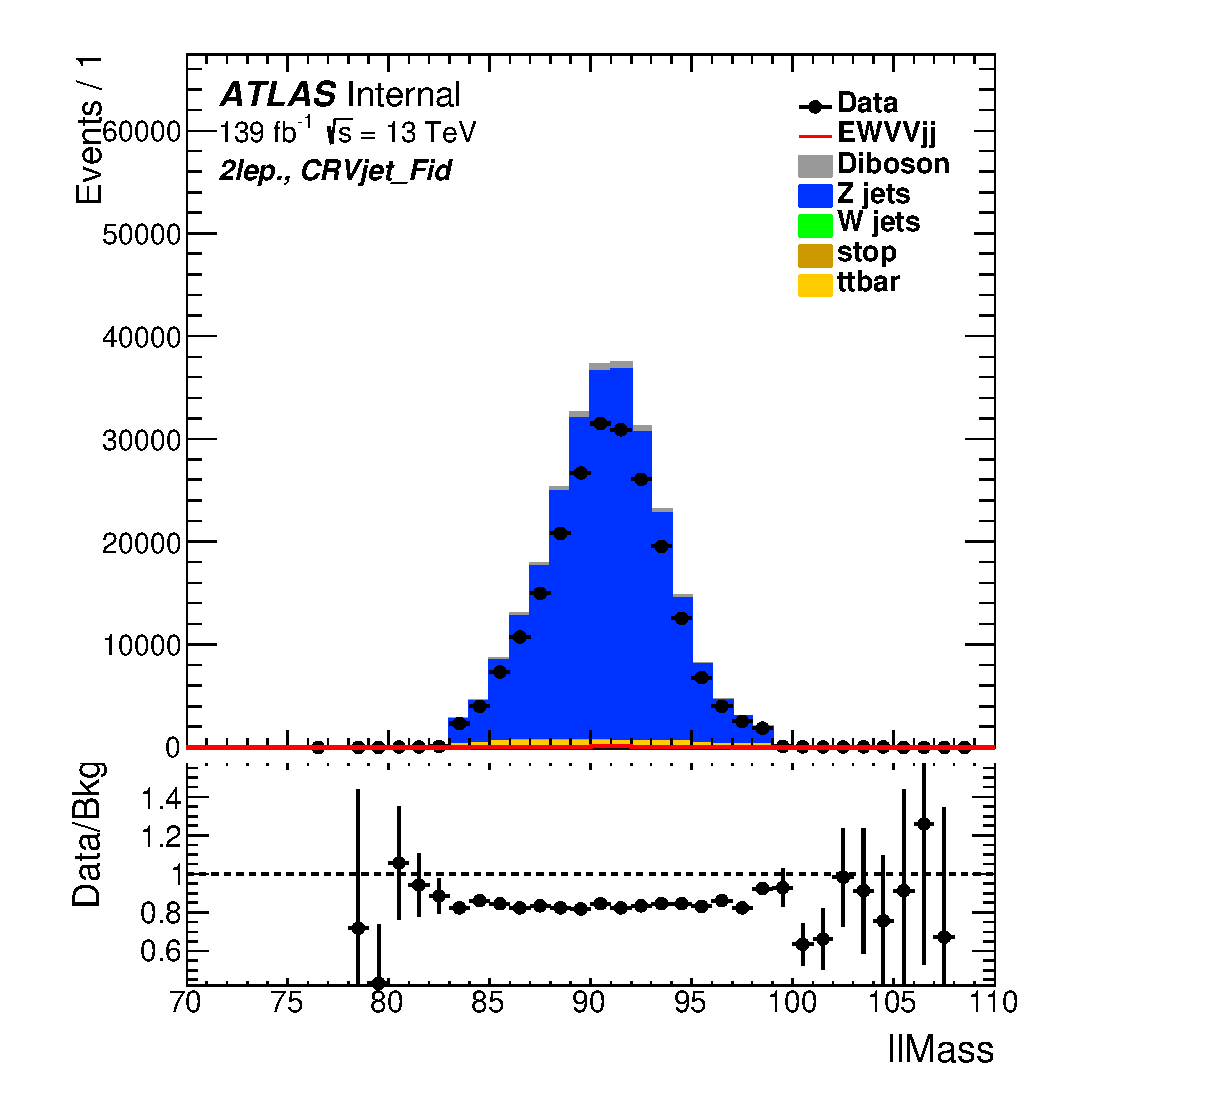
\includegraphics[width=0.45\textwidth]{figures/2lep/reweighting/after_reweighting/C_0ptag2pjet_0ptv_CRVjet_Fid_llMass_Lin.eps}}
%    \subfigure[]{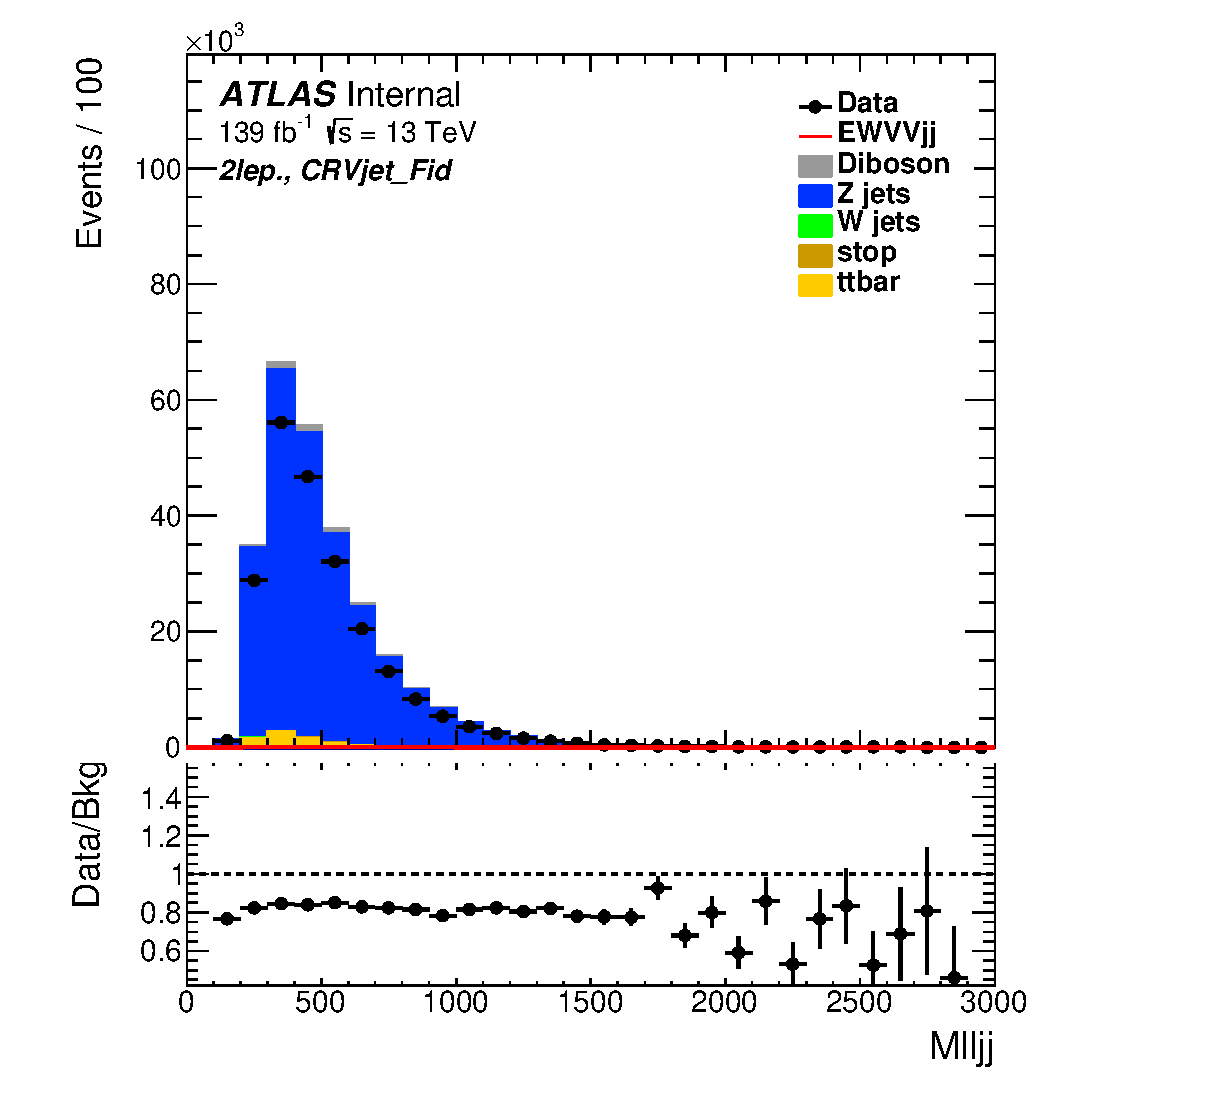
\includegraphics[width=0.45\textwidth]{figures/2lep/reweighting/after_reweighting/C_0ptag2pjet_0ptv_CRVjet_Fid_Mlljj_Lin.eps}}
%    \subfigure[]{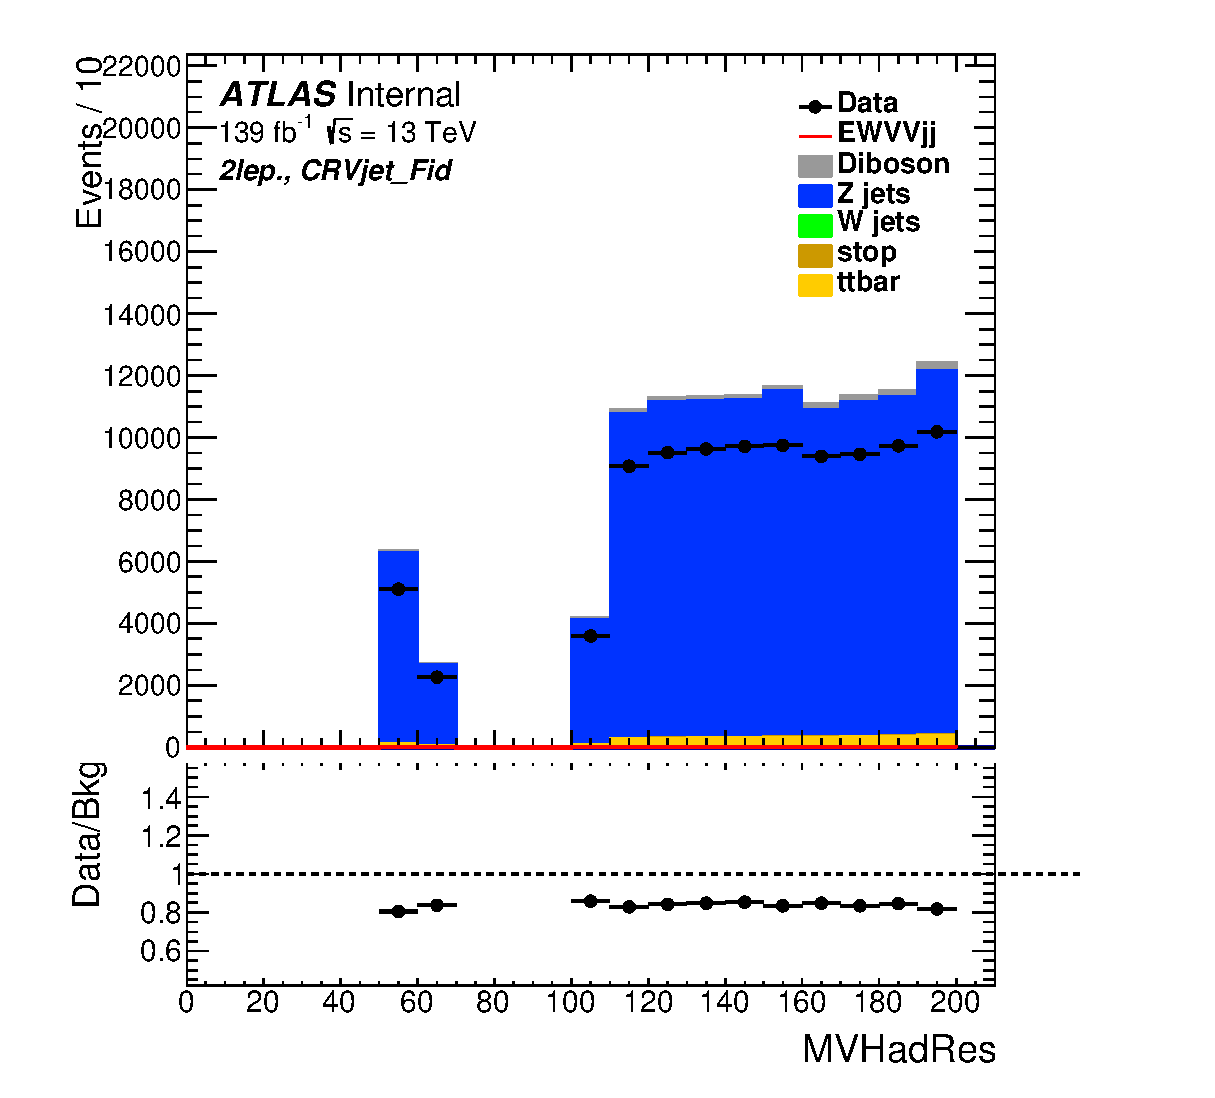
\includegraphics[width=0.45\textwidth]{figures/2lep/reweighting/after_reweighting/C_0ptag2pjet_0ptv_CRVjet_Fid_MVHadRes_Lin.eps}}
%    \subfigure[]{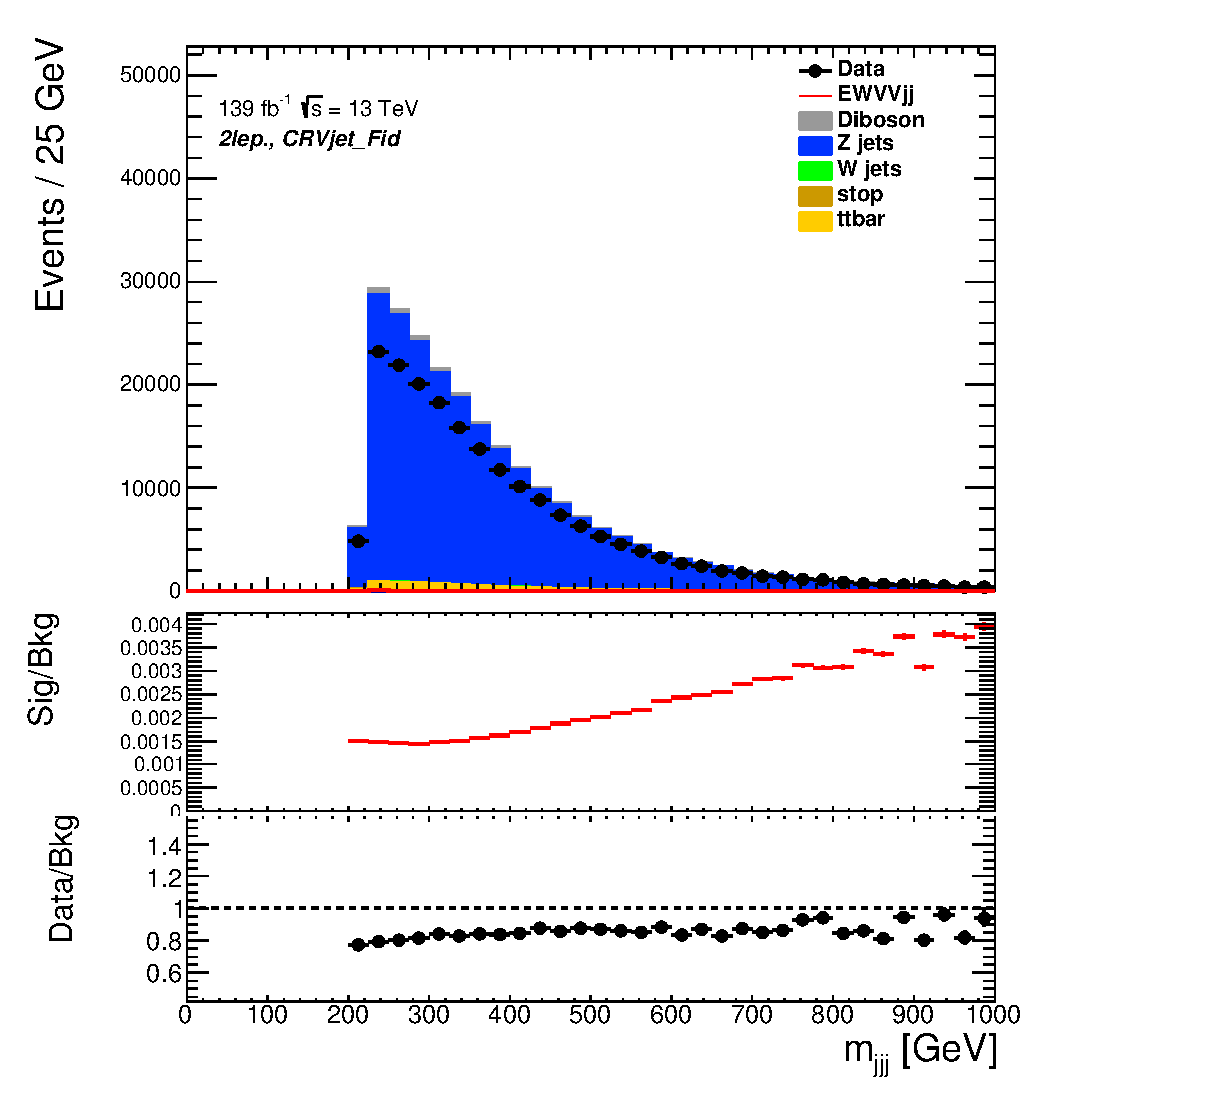
\includegraphics[width=0.45\textwidth]{figures/2lep/reweighting/after_reweighting/C_0ptag2pjet_0ptv_CRVjet_Fid_topMass_Lin.eps}}
 %   \caption{ Various kinematic variables in the Z+jets resolved CR in the 2-lepton channel analysis.}
  %  \label{fig:2lep_zjets_resolved_CR}
%\end{figure}


\chapter{Statistical treatment}

\section{Likelihood function definition}
A binned maximum likelihood fit is performed to get the signal strength $\mu$. The likelihood function is written as:
\begin{equation} \label{eq:Lh1}
\mathcal{L}\left( N, \tilde{\theta} | \mu, \theta \right)=  P\left( \mu | \mu s +b \right) \cdot p\left( \tilde{\theta} | \theta \right)
 \end{equation}
 
 $P$ is the Poisson probability terms over all the histogram bins:

 \begin{equation} \label{eq:Lh2}
 P\left( \mu | \mu s +b \right)  =  \prod_{i=1}^{N_{bins}} \frac{{ (\mu s_{i} (\theta)+ b_{i}(\theta))^{N_{i}} e^{ - (\mu s_{i}(\theta) + b_{i}(\theta))} } }{{N_{i}!}}
 \end{equation}

where $\mu s_{i }$, $b_{i }$ is the expected number of signal and background events in bin i, and $N_{i}$ is the number of observed events in the bin. 
The $p\left( \tilde{\theta} | \theta \right)$ term of equation~\ref{eq:Lh1} is added to represent the additional systematic effects considered in the analysis. This term is usually referred to as prior. 

Assuming not correlated uncertainties, this term is given by the product of all single uncertainty priors; $ p\left( \tilde{\theta} | \theta \right) =  \prod_{j}p_{j}\left( \tilde{\theta_{j}} | \theta_{j} \right)$, where j is running over all uncertainties and  $\theta_{j}$ is the nuisance parameter associated to the source of systematic uncertainty j. Each of the terms represents the probability of the uncertainty to have a true value equal to $\theta_{j}$ given the best estimate $ \tilde{\theta_j}$ obtained from an auxiliary measurement. 
In this analysis, priors are considered to be Gaussian distributed for the majority of uncertainties. $\theta_{j} $ are scaled to $\theta_{j} =0$ for the nominal expectation, and $\theta_{j} = \pm 1$ is scaled to the $\pm 1 \sigma$ variations of the systematic source.




%corresponds to the nominal expectation while $\theta_{j} = \pm 1$ correspond to the $\pm 1 \sigma$ variations of the systematic source. 

%This parametrization is convenient in order to easily spot constrained nuisance parameters that might be problematic. %Log-normal priors are also used in the case of uncertainties with only normalizations effects. % An estimate on $\mu$ is obtained by maximizing the likelihood function with respect to all the parameters.

\section{Smoothing}
The smoothing algorithm is applied to alleviate statistical fluctuations, that might create suspicious effects in the fit.
During this procedure bins are migrated from left to right until the statistical uncertainty per bin to be less than 5$\%$. The nominal and smoothed variation histograms are then compared to derive the up and down uncertainties. The resulting uncertainties are associated to the initial finer binned distribution. 

\section{Pruning}
Systematic variations that have a very small effect and are negligible for the measurement are pruned away. The uncertainties removed are:
  \begin{itemize}
   \item  Normalization uncertainties with a less than 5$\%$ relative variation effects or same sign effects (relative variation being positive (or negative) for both the up and down uncertainty)
   \item  Shape uncertainties with less than 0.5$\%$ effect for all bins of the distribution or missing one of the up or down variations.
    \end{itemize}
    
The nominal fit result in terms of $\mu$ and $\sigma_{\mu}$ is obtained by maximizing the likelihood function with respect to all parameters.
%This is referred to as the maximized log-likelihood value, MLL.
%The test statistic $q_\mu$ is then constructed according to the profile likelihood: $q_\mu = 2 \ln (\mathcal{L} (\mu, \hat{\hat{\theta_\mu}})/\mathcal{L} (\hat{\mu}, \hat{\theta}))$, where $\hat{\mu}$ and $\hat{\theta}$ are the parameters that maximize the likelihood (with the constraint $0 \leq \hat{\mu} \leq \mu$), and $\hat{\hat{\theta}}_\mu$ are the nuisance parameter values that maximize the likelihood for a given $\mu$.
%This test statistic is used to measure the compatibility of the background-only model with the observed data and for exclusion intervals derived with the $CL_s$ method~\cite{Cowan:2010js}.
%The limit set on $\mu$ is then translated into a limit on the signal cross section times branching ratio, using the theoretical cross section and branching ratio for the given signal model.

\section{Fitting strategy}
A simultaneous fit to the merged and resolved signal and control regions is performed. In the signal regions the RNN score is fitted, while in the CRs the $M^{tag}_{jj}$ is fitted, in order to give a better constrains to the $M^{tag}_{jj}$ reweighting uncertainty. The 2POI fit to the Merged and Resolved region is also performed as a testing purpose. For the blinding strategy, unconditional fits on the Asimov dataset are performed in the full range of the RNN score. Unconditional fit on data are also performed to the left-side bins of the RNN score up to the 75\% of the total signal integral.




\chapter{Systematic uncertainties}
In this section, all systematic uncertainties considered in the analysis are described. The uncertainties are divided into three categories:
Experimental uncertainties, Background modeling uncertainties, Theoretical uncertainties. Each systematic uncertainty is treated as a nuisance parameter as described in Chapter{}. The systematic variations are estimated on the final discriminant described in Chapter{}.

\section{Experimental uncertainties}

\begin{table}[!hp]
  \centering
  \footnotesize
  \begin{center}
    \begin{tabular}{|l|l|l|}
      \hline
      Source        & Description                     & Analysis Name                                       \\ \hline
      Small-R Jets  &             &  JET\_CR\_JET\_BJES\_Response                            \\
      Small-R Jets  &             &  JET\_CR\_JET\_EffectiveNP\_Detector1                    \\
      Small-R Jets  &             &  JET\_CR\_JET\_EffectiveNP\_Detector2                    \\
      Small-R Jets  &             &  JET\_CR\_JET\_EffectiveNP\_Mixed1                       \\
      Small-R Jets  &             &  JET\_CR\_JET\_EffectiveNP\_Mixed2                       \\
      Small-R Jets  &             &  JET\_CR\_JET\_EffectiveNP\_Mixed3                       \\
      Small-R Jets  &             &  JET\_CR\_JET\_EffectiveNP\_Modelling1                   \\
      Small-R Jets  &             &  JET\_CR\_JET\_EffectiveNP\_Modelling2                   \\
      Small-R Jets  &             &  JET\_CR\_JET\_EffectiveNP\_Modelling3                   \\
      Small-R Jets  &             &  JET\_CR\_JET\_EffectiveNP\_Modelling4                   \\
      Small-R Jets  &             &  JET\_CR\_JET\_EffectiveNP\_Statistical1                 \\
      Small-R Jets  &             &  JET\_CR\_JET\_EffectiveNP\_Statistical2                 \\
      Small-R Jets  &             &  JET\_CR\_JET\_EffectiveNP\_Statistical3                 \\
      Small-R Jets  &             &  JET\_CR\_JET\_EffectiveNP\_Statistical4                 \\
      Small-R Jets  &             &  JET\_CR\_JET\_EffectiveNP\_Statistical5                 \\
      Small-R Jets  &             &  JET\_CR\_JET\_EffectiveNP\_Statistical6                 \\
      Small-R Jets  &             &  JET\_CR\_JET\_Flavor\_Composition                       \\
      Small-R Jets  &             &  JET\_CR\_JET\_Flavor\_Response                          \\
      Small-R Jets  &             &  JET\_CR\_JET\_Pileup\_OffsetMu                          \\
      Small-R Jets  &             &  JET\_CR\_JET\_Pileup\_OffsetNPV                         \\
      Small-R Jets  &             &  JET\_CR\_JET\_Pileup\_PtTerm                            \\
      Small-R Jets  &             &  JET\_CR\_JET\_Pileup\_RhoTopology                       \\
      Small-R Jets  &             &  JET\_CR\_JET\_PunchThrough\_MC16                        \\
      Small-R Jets  &             &  JET\_CR\_JET\_SingleParticle\_HighPt                    \\
      Small-R Jets  &  the scale of forward jets w.r.t. central jets  &  JET\_CR\_JET\_EtaIntercalibration\_TotalStat            \\
      Small-R Jets  &               &  JET\_CR\_JET\_EtaIntercalibration\_Modelling            \\
      Small-R Jets  &             &  JET\_CR\_JET\_EtaIntercalibration\_NonClosure\_highE    \\
      Small-R Jets  &             &  JET\_CR\_JET\_EtaIntercalibration\_NonClosure\_negEta   \\
      Small-R Jets  &             &  JET\_CR\_JET\_EtaIntercalibration\_NonClosure\_posEta   \\
      \hline
      Small-R Jets  & JER                  &  JET\_CR\_JET\_JER\_DataVsMC                 \\
      Small-R Jets  & JER                  &  JET\_CR\_JET\_JER\_EffectiveNP\_1           \\
      Small-R Jets  & JER                  &  JET\_CR\_JET\_JER\_EffectiveNP\_2           \\
      Small-R Jets  & JER                  &  JET\_CR\_JET\_JER\_EffectiveNP\_3           \\
      Small-R Jets  & JER                  &  JET\_CR\_JET\_JER\_EffectiveNP\_4           \\
      Small-R Jets  & JER                  &  JET\_CR\_JET\_JER\_EffectiveNP\_5           \\
      Small-R Jets  & JER                  &  JET\_CR\_JET\_JER\_EffectiveNP\_6           \\
      Small-R Jets  & JER                  &  JET\_CR\_JET\_JER\_EffectiveNP\_7restTerm   \\
      \hline
  \end{tabular}
  \end{center}
\end{table}


\subsection*{Small-$R$ Jet Energy Scale(JES) and Resolution(JER) Uncertainty}
The jet energy scale (JES) uncertainties and jet energy resolution (JER) are measured by calculating the response between MC and data in various kinematic phase space ~\cite{JetUncertainties}.
What is used in this analysis is 30 JES uncertainty and 8 JER uncertainty components.
We also consider the uncertainty on jet vertex tagger (JVT) efficiency~\cite{JVTCalib} and forward jet vertex tagger (fJvt) efficiency.
%We use the configuration \texttt{R4\_CategoryReduction\_SimpleJER.config}



\subsection*{Large-$R$ Jet Energy Scale and Resolution Uncertainty}
\label{sec:fatjetUncert}

The large-$R$ jet energy scale uncertainties are included following the prescription of the
jet substructure group included in the \texttt{JetUncertainties} package~\cite{JSSrecommendation}.
The uncertainty on the \pt scale of jets is evaluated by
comparing the ratio of the jet \pt to track-jet \pt in dijet data and simulation (Rtrk method).
In addition to this ``Baseline'' uncertainty, the uncertainties on track measurements (``Tracking''), differences between Pythia and Sherpa dijet simulations (``Modelling'') and the statistical uncertainty of dijet data (``TotalStat'') are considered.

  \begin{table}[!hp]
  \centering
  \footnotesize
  \begin{center}
    \begin{tabular}{|l|l|l|}
      \hline
      Source        & Description                     & Analysis Name                                       \\ \hline
      Large-R Jets  & \pt scale                       & FATJET\_Medium\_JET\_Rtrk\_Baseline\_pT              \\
      Large-R Jets  & \pt scale                       & FATJET\_Medium\_JET\_Rtrk\_Modelling\_pT             \\
      Large-R Jets  & \pt scale                       & FATJET\_Medium\_JET\_Rtrk\_TotalStat\_pT             \\
      Large-R Jets  & \pt scale                       & FATJET\_Medium\_JET\_Rtrk\_Tracking\_pT              \\

      Large-R Jets  & \pt scale                       & FATJET\_BJT\_JET\_EtaIntercalibration\_Modelling      \\
      Large-R Jets  & \pt scale                       & FATJET\_BJT\_JET\_Flavor\_Composition                 \\
      Large-R Jets  & \pt scale                       & FATJET\_BJT\_JET\_Flavor\_Response                    \\

      Large-R Jets  & Mass resolution                 & FATJET\_JMR                            \\\hline
      Large-R Jets  & JER                             & FATJET\_JER                            \\\hline
\end{tabular}
    \end{center}
  \caption{ Qualitative summary of the systematic uncertainties included in this analysis. }
  \label{tab:syst_summary_sources_3}
  \end{table}

  \clearpage
  
  All other experimental uncertainties are summerized in the Table{}.

\subsection*{Luminosity}
The uncertainty on the integrated luminosity. 
For the 2015+2016 dataset, this uncertainty is 2.1\%, and 2.4\% for the 2017 dataset. The uncertainty for the 2018 data alone is 2.0\%, and the uncertainty for the combined run-2 dataset (2015-2018) is 1.7\% \cite{AtlasLumiRun2}.
The luminosity uncertainty is applied to all MC samples.
\subsection*{Pileup reweighting}
The uncertainty associated with the pileup reweighting is considered\cite{ExtendedPileupReweighting}. To cover the uncertainty on the ratio between the predicted and measure inelastic cross-section in the fiducial volume is covered. The fiducial volume is defined by $M_X > 13\,\GeV$ where $M_X$ is the mass of the non-diffractive hadronic system~\cite{STDM-2015-05}.

 \begin{table}[!hp]
  \centering
  \footnotesize
  \begin{center}
    \begin{tabular}{|l|l|l|l|}
      \hline
      Source             & Description   & Analysis Name    \\ \hline
      Luminosity         & LumiNP        & ATLAS\_LUMI\_2015\_2018 \\ \hline
      Pileup reweighting & PRW\_DATASF   & PRW\_DATASF       \\\hline       
    \end{tabular}
    \end{center}
  \label{tab:syst_summary_sources_1}
 \end{table}



\subsection*{Muons and electrons}
The following systematic uncertainties are applied to electrons and muons in estimations based on the simulation:

\begin{itemize}
\item Identification and reconstruction efficiencies: The efficiencies are measured with the tag and probe method using the $Z$ mass peak.
\item Isolation efficiency: Scale factor and its uncertainty are derived by tag and probe method using the $Z$ mass peak as well.
\item Energy and Momentum scales: These are also measured with $Z$ mass line shape, and provided by the CP groups.
\item Track-to-vertex association efficiency: Only for muons.
\end{itemize}

They are implemented in \texttt{ElectronPhotonFourMomentumCorrection}~\cite{EgammaCalibration},\\
\texttt{ElectronEfficiencyCorrection}~\cite{AsgElectronEfficiencyCorrectionTool}, \\
\texttt{MuonMomentumCorrections} and \texttt{MuonEfficiencyCorrections}~\cite{MCPAnalysisGuidelines}.


\subsection*{Missing transverse energy}
 The missing transverse energy is calculated using physics objects as described in Section~\ref{sec:ObjectDefinition}.
%from the negative vectorial sum of physics objects: muons, electrons, taus, photons, jets and unassociated clusters of calorimeter cells.
As such, all of the systematic errors on the reconstructed components, e.g. the jet energy scale,
result in an uncertainty on $\met$. These are the dominant sources of uncertainty on $\met$.
In addition, there is an uncertainty called the ''Soft Term'', from the unassociated tracks.
The resolution and scale of this soft term are varied within their errors to evaluate their
contribution to the total uncertainty using \texttt{METUtilities}~\cite{METUtilSystematics}.

\begin{table}[!hp]
  \centering
  \footnotesize
  \begin{center}
    \begin{tabular}{|l|l|l|}
      \hline
      Source        & Description                     & Analysis Name                                 \\ \hline
      Electrons     & Energy scale                    &  EG\_SCALE\_ALL                               \\
      Electrons     & Energy resolution               &  EG\_RESOLUTION\_ALL                          \\
      Electrons     & Trigger                         &  EL\_EFF\_Trigger\_TOTAL\_1NPCOR\_PLUS\_UNCOR  \\
      Electrons     & ID efficiency SF                &  EL\_EFF\_ID\_TOTAL\_1NPCOR\_PLUS\_UNCOR      \\
      Electrons     & Isolation efficiency SF         &   EL\_EFF\_Iso\_TOTAL\_1NPCOR\_PLUS\_UNCOR   \\
      Electrons     & Reconstruction efficiency SF    &   EL\_EFF\_Reco\_TOTAL\_1NPCOR\_PLUS\_UNCOR   \\ \hline
      Muons         & \pt\ scale                      &   MUONS\_SCALE                                \\
      Muons         & \pt\ scale (charge dependent)   &   MUON\_SAGITTA\_RHO                    \\
      Muons         & \pt\ scale (charge dependent)          &   MUON\_SAGITTA\_RESBIAS                \\
      Muons         & \pt\ resolution MS               &   MUONS\_MS                                   \\
      Muons         & \pt\ resolution ID               &   MUONS\_ID                                   \\
      Muons         & Isolation efficiency SF         &   MUON\_ISO\_SYS                               \\
      Muons         & Isolation efficiency SF         &   MUON\_ISO\_STAT                               \\
      Muons         & Muon reco \& ID efficiency SF               &   MUONS\_EFF\_STAT                  \\
      Muons         & Muon reco \& ID efficiency SF               &   MUONS\_EFF\_STAT\_LOWPT           \\
      Muons         & Muon reco \& ID efficiency SF               &   MUONS\_EFF\_SYST                  \\
      Muons         & Muon reco \& ID efficiency SF               &   MUONS\_EFF\_SYST\_LOWPT           \\
      Muons         & Track-to-vertex association efficiency SF         &   MUON\_TTVA\_SYS             \\
      Muons         & Track-to-vertex association efficiency SF         &   MUON\_TTVA\_STAT            \\ \hline
      MET           & Soft term                       &   MET\_SoftTrk\_ResoPerp                        \\
      MET           & Soft term                       &   MET\_SoftTrk\_ResoPara                        \\
      MET           & Soft term                       &   MET\_SoftTrk\_Scale                           \\ \hline
      \end{tabular}
      \caption{ Qualitative summary of the systematic uncertainties included in this analysis. }
      \label{tab:syst_summary_sources_2}
    \end{center}
  \end{table}

\subsection{B-tagging uncertainties}
The systematic uncertainties associated to the b-tagging.
They are uncertainties on the scaling factor for taking account for the disagreement of the b-tag efficiency between data and MC. Each separated scale factors and corresponding systematic uncertainties are provided for b-,c-, and light-flavor jets from several measurements.
These b-tagging systematic uncertainties are applied when calculating the SF since they are uncertainties on the SF. b-tagging SF is firstly calculated with all small-R jets (PFlowJets) and applied to the events after having selected non b-tagged tagging jets, same as the uncertainties. 

\begin{table}[!hp]
  \centering
  \footnotesize
  \begin{center}
    \begin{tabular}{|l|l|l|}
      \hline
      Source        & Description                     & Analysis Name  \\ \hline
      B-tagging     & Flavor tagging scale factors    &  FT\_EFF\_Eigen\_B\_0\_AntiKt4PFlowJets                \\
      B-tagging     & Flavor tagging scale factors    &  FT\_EFF\_Eigen\_B\_1\_AntiKt4PFlowJets                \\
      B-tagging     & Flavor tagging scale factors    &  FT\_EFF\_Eigen\_B\_2\_AntiKt4PFlowJets                \\
      B-tagging     & Flavor tagging scale factors    &  FT\_EFF\_Eigen\_C\_0\_AntiKt4PFlowJets                \\
      B-tagging     & Flavor tagging scale factors    &  FT\_EFF\_Eigen\_C\_1\_AntiKt4PFlowJets                \\
      B-tagging     & Flavor tagging scale factors    &  FT\_EFF\_Eigen\_C\_2\_AntiKt4PFlowJets                \\
      B-tagging     & Flavor tagging scale factors    &  FT\_EFF\_Eigen\_C\_3\_AntiKt4PFlowJets                \\
      B-tagging     & Flavor tagging scale factors    &  FT\_EFF\_Eigen\_Light\_0\_AntiKt4PFlowJets            \\
      B-tagging     & Flavor tagging scale factors    &  FT\_EFF\_Eigen\_Light\_1\_AntiKt4PFlowJets            \\
      B-tagging     & Flavor tagging scale factors    &  FT\_EFF\_Eigen\_Light\_2\_AntiKt4PFlowJets            \\
      B-tagging     & Flavor tagging scale factors    &  FT\_EFF\_Eigen\_Light\_3\_AntiKt4PFlowJets            \\
      B-tagging     & Flavor tagging scale factors    &  FT\_EFF\_extrapolation\_AntiKt4PFlowJets              \\
      B-tagging     & Flavor tagging scale factors    &  FT\_EFF\_extrapolation\_from\_charm\_AntiKt4PFlowJets \\ \hline
\end{tabular}
    \end{center}
  \caption{ Qualitative summary of the systematic uncertainties included in this analysis. }
  \label{tab:syst_summary_sources_4}
  \end{table}

\subsection{Quark/Gluon jets uncertainties}
The Flavour response and the Flavour conposition uncertatinties.
\subsection{Background Modeling uncertainties}
The systematics uncertainties related to the modeling of the background samples are explained.
By thinking of this, the the difference of the parton shower modeling is considered as the difference of Phythia and Herwig.
\subsection{Reweighting uncertainties}

\section{Theoretical uncertainties}
The systematic uncertainties related to the determination or the calculation of the MC.

\subsection{Perturbative QCD matrix-element uncertainties}
\begin{itemize}
\item PDF + $\alpha_s$ uncertainties\\
Since PDF sets are obtained by fitting experimental dataset, there are uncertainties on selecting different type of PDF sets, which originated from the experimental uncertainties from the dataset and from the choice of the functional form adapted in the PDF fits.
The uncertainty from the PDF set choice can be assessed by 2 means. One is by calculating the difference within one PDF set by varying its internal parameters, which is called internal PDF uncertainties. The second is from the difference between the nominal sets of different PDF sets, which is called external PDF uncertainties.
$\alpha_s$ uncertainties are from the experimental uncertainties in the determination of it and the truncated fixed order calculations are used for the calculation.
\item QCD scale uncertainties\\
QCD scale uncertainties are determined by using different renormalization and factorization scale factor sets. 
The renormalization scale $\mu_R$ is the scale at which the strong coupling $\alpha_s$ is evaluated, while the factorization scale $\mu_F$ is the scale to separate the perturbative part of the hard-interaction from the non-perturbative part of PDF. 


\subsection{NLO order EW corrections}
\color{blue}
this is not currently considered
\end{itemize}


%%% aQGC %%%
\chapter{Interpretation with Effective Field Theory}
\label{chap:aQGC}

%\subsection{Introduction}
%The boson field self-interactions respect the $SU(2)\times U(1)_Y$ gauge invariance in the electroweak sector of the SM and serve as a very sensitive tool to search for the manifestations of physics beyond the SM.
%The VBS is one of the processes directly sensitive to the quartic-gauge coupling vertices of the SM.
%Variations of these vertices from the SM are known as anomalous quartic-gauge couplings (aQGC), and can arise from alterations of the electroweak or Higgs sector of the SM.
%The effect of such new physics introduced by aQGC can be realized using the effective field theory~\cite{degrande2013effective} and linearly parameterized by the effective Lagrangian as:
%\begin{equation*}
%  \mathcal{L}=\mathcal{L}_{sm}+\sum_{i}\frac{c_i}{\Lambda^{2}}\mathcal{L}_i+\sum_{n}\frac{f_n}{\Lambda^{4}}\mathcal{L}_n,
%\end{equation*}
%where $\mathcal{L}$ represents possible dim-6 and dim-8 operators and $c_i$ and $f_n$ are correspond their Wilson coefficients. The $\Lambda$ represents the energy scale over which the new degrees of freedom are integrated out. 
%In this note, the name of Lagrangian term that contains the given operator is denoted by its Wilson coefficient i.e. $L_{n} = \frac{f_{n}}{\Lambda^4} O_{n}$ is called as $f_{n}$.
%The odd-dimension operators violate lepton and baryon number conservation and are ignored.
%Both of dim-6 and dim-8 operators can contribute to the VBS processes through aTGC and aQGC, respectively,
%but due to the tight constraints of dim-6 operators from inclusive diboson measurements, only dim-8 operators are discussed in this note.
%The Eboli model~\cite{eboli2006p} is employed to describe the signals, which introduces twentyone new dim-8 operators satisfying the SM $SU(2)\times U(1)_Y$ symmetry. 
%These operators can be categorized by the types of the coupling; scalar types that contain just covariant derivatives of the Higgs field: $f_{S0}$, $f_{S1}$, $f_{S2}$, tensor types  that contain just field strengths: $f_{T0}$, ..., $f_{T9}$, and mixed operators that exhibit two covariant derivatives of the Higgs field and two field strengths: $f_{M0}$, ..., $f_{M7}$. 
%Table~\ref{tab:operators} shows the vertices that can be modified by the given operator. 
%The operators $f_{S0}$ and $f_{S2}$ are Hermitian conjugates, so they are treated as one single operator by setting both coefficients to be the same value.
%The semileptonic VBS is a golden channel that can test nineteen oeperators simultaneously, which has  $WW$, $WZ$, and $ZZ$ pairs in the final state.
%It is found via simulations that the tensor operators produce purely transversely polarized $W/Z$ bosons, while the scalar operators longitudinal bosons.
%In particular in the merged analysis, higher selection efficiency for the scalar operators is expected since the boosted boson tagger is optimized for the logitudinally-polarized bosons.

%\begin{table}[ht!]
%\begin{center}
%\resizebox{0.70\textwidth}{!}{
%\begin{tabular}{|c|c|c|c|c|c|c|c|c|c|}
%\hline & WWWW & WWZZ & ZZZZ & WWAZ & WWAA & ZZZA & ZZAA & ZAAA & AAAA \\
%\hline $\mathcal{L}_{S02}, \mathcal{L}_{S1}$ & $\mathrm{X}$ & $\mathrm{X}$ & $\mathrm{X}$ & %$\mathrm{O}$ & $\mathrm{O}$ & $\mathrm{O}$ & $\mathrm{O}$ & $\mathrm{O}$ & $\mathrm{O}$ \\
%\hline $\mathcal{L}_{M0}, \mathcal{L}_{M1}, \mathcal{L}_{M6}, \mathcal{L}_{M7}$ & $\mathrm{X}$ & %$\mathrm{X}$ & $\mathrm{X}$ & $\mathrm{X}$ & $\mathrm{X}$ & $\mathrm{X}$ & $\mathrm{X}$ & %$\mathrm{O}$ & $\mathrm{O}$ \\
%\hline $\mathcal{L}_{M2}, \mathcal{L}_{M3}, \mathcal{L}_{M4}, \mathcal{L}_{M5}$ & $\mathrm{O}$ & %$\mathrm{X}$ & $\mathrm{X}$ & $\mathrm{X}$ & $\mathrm{X}$ & $\mathrm{X}$ & $\mathrm{X}$ & %$\mathrm{O}$ & $\mathrm{O}$ \\
%\hline $\mathcal{L}_{T0}, \mathcal{L}_{T1}, \mathcal{L}_{T2}$ & $\mathrm{X}$ & $\mathrm{X}$ & %$\mathrm{X}$ & $\mathrm{X}$ & $\mathrm{X}$ & $\mathrm{X}$ & $\mathrm{X}$ & $\mathrm{X}$ & %$\mathrm{X}$ \\
%\hline $\mathcal{L}_{T5}, \mathcal{L}_{T6}, \mathcal{L}_{T7}$ & $\mathrm{O}$ & $\mathrm{X}$ & %$\mathrm{X}$ & $\mathrm{X}$ & $\mathrm{X}$ & $\mathrm{X}$ & $\mathrm{X}$ & $\mathrm{X}$ & %$\mathrm{X}$ \\
%\hline $\mathcal{L}_{T8}, \mathcal{L}_{T9}$ & $\mathrm{O}$ & $\mathrm{O}$ & $\mathrm{X}$ & $\mathrm{O}$ & $\mathrm{O}$ & $\mathrm{X}$ & $\mathrm{X}$ & $\mathrm{X}$ & $\mathrm{X}$ \\
%\hline
%\end{tabular}
%}
%\caption{Correspondences between Wilson coefficients and vertices. $\mathrm{X}$ shows the existence of the vertex with the interaction by the operator.}
%\label{tab:operators}
%\end{center}
%\end{table}

As mentioned in Section~\ref{subsec:EFT}, aQGC interpretation is done via EFT lagrangian. 
The SM+EFT matrix element can be written as
\begin{equation}
   |A_{SM}+\frac{f_i}{\Lambda^4}A_i|^2=|A_{SM}|^2+\sum\limits_i \frac{f_i^2}{\Lambda^8}|A_{i}|^2+ \sum\limits_i 2 \frac{f_i}{\Lambda^4} \mathrm{Re}(A_{SM}^\star A_i) +\sum\limits_{i\neq j} \frac{f_i}{\Lambda^4} \frac{f_j}{\Lambda^4} \mathrm{Re}(A_i^\star A_j)
\end{equation}
where $|A_SM|^2$ is the SM matrix element, $|A_{i}|^2$ represents the pure-EFT matrix elements for the $f_{i}$ operator, $2 \mathrm{Re}(A_{SM}^\star A_i)$ is its corresponding interference term with the SM, and $\mathrm{Re}(A_i^\star A_j)$ is possible interference term between EFT operators $f_{i}$ and $f_{j}$. 
Theoretically, it cannot separate the effects of Wilson coefficients $f_i$ and the scale $\Lambda^4$, so the parameter of interest in this analysis is the ratio $\frac{f_i}{\Lambda^4}$. %Sometimes it is just called as $f_i$.
The pure-EFT term is scaled by the quadrature of $\frac{f_i}{\Lambda^4}$ and the interference term by $\frac{f_{i}}{\Lambda^4}$.
Sometimes they are called as the quadratic term and the interference (linear) term, respectively.

\section{Statistical interpretation}
The aQGC signal is extracted with a profile-likelihood fit same as what is described in section~\ref{sec:likelihood}, where the signal referring to the aQGC signal sample, and the standard model EW VV+jj signal sample is included as background with other standard model background samples like V+jets and $t\bar{t}$.
The signal strength, $\mu$ is interpreted in terms of Wilson coefficient, $\mu$ = $\frac{f_i}{\Lambda^4}$. 
The POI is set to include both quadratic terms and interference terms simultaneously, thereby two signal strength is parameterized as $\mu_{QUAD} = \mu_{INT}^2$.
Figure~\ref{fig:quadint} shows the quadratic and interference signal distributions of di-boson invariant mass ($m_{VV}$) in HP SR, which has the most signal constraining power in 2-lepton channel.
\begin{figure}[ht]
    \centering
        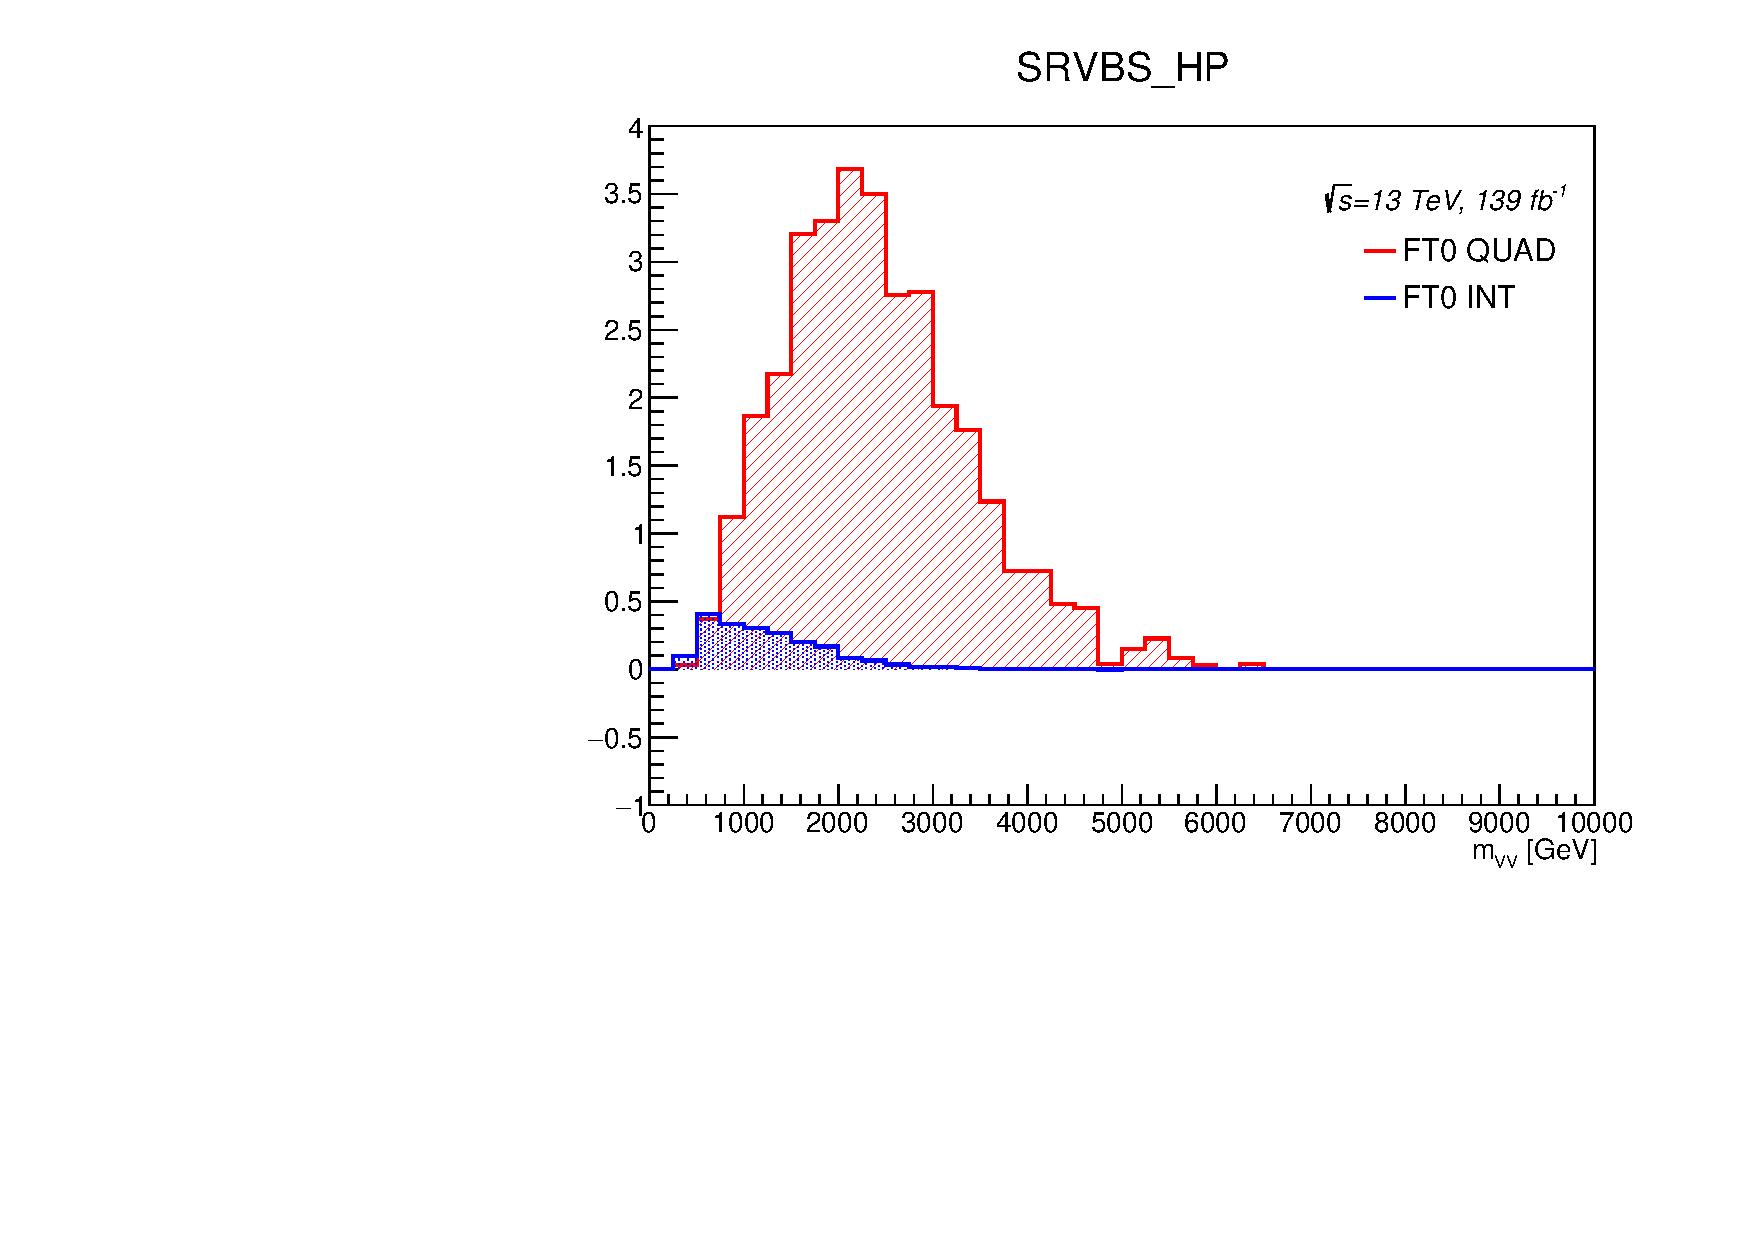
\includegraphics[width=0.45\textwidth]{figures/aQGC/FT0_0ptag1pfat0pjet_0ptv_SRVBS_HP_MllJ.pdf}
    	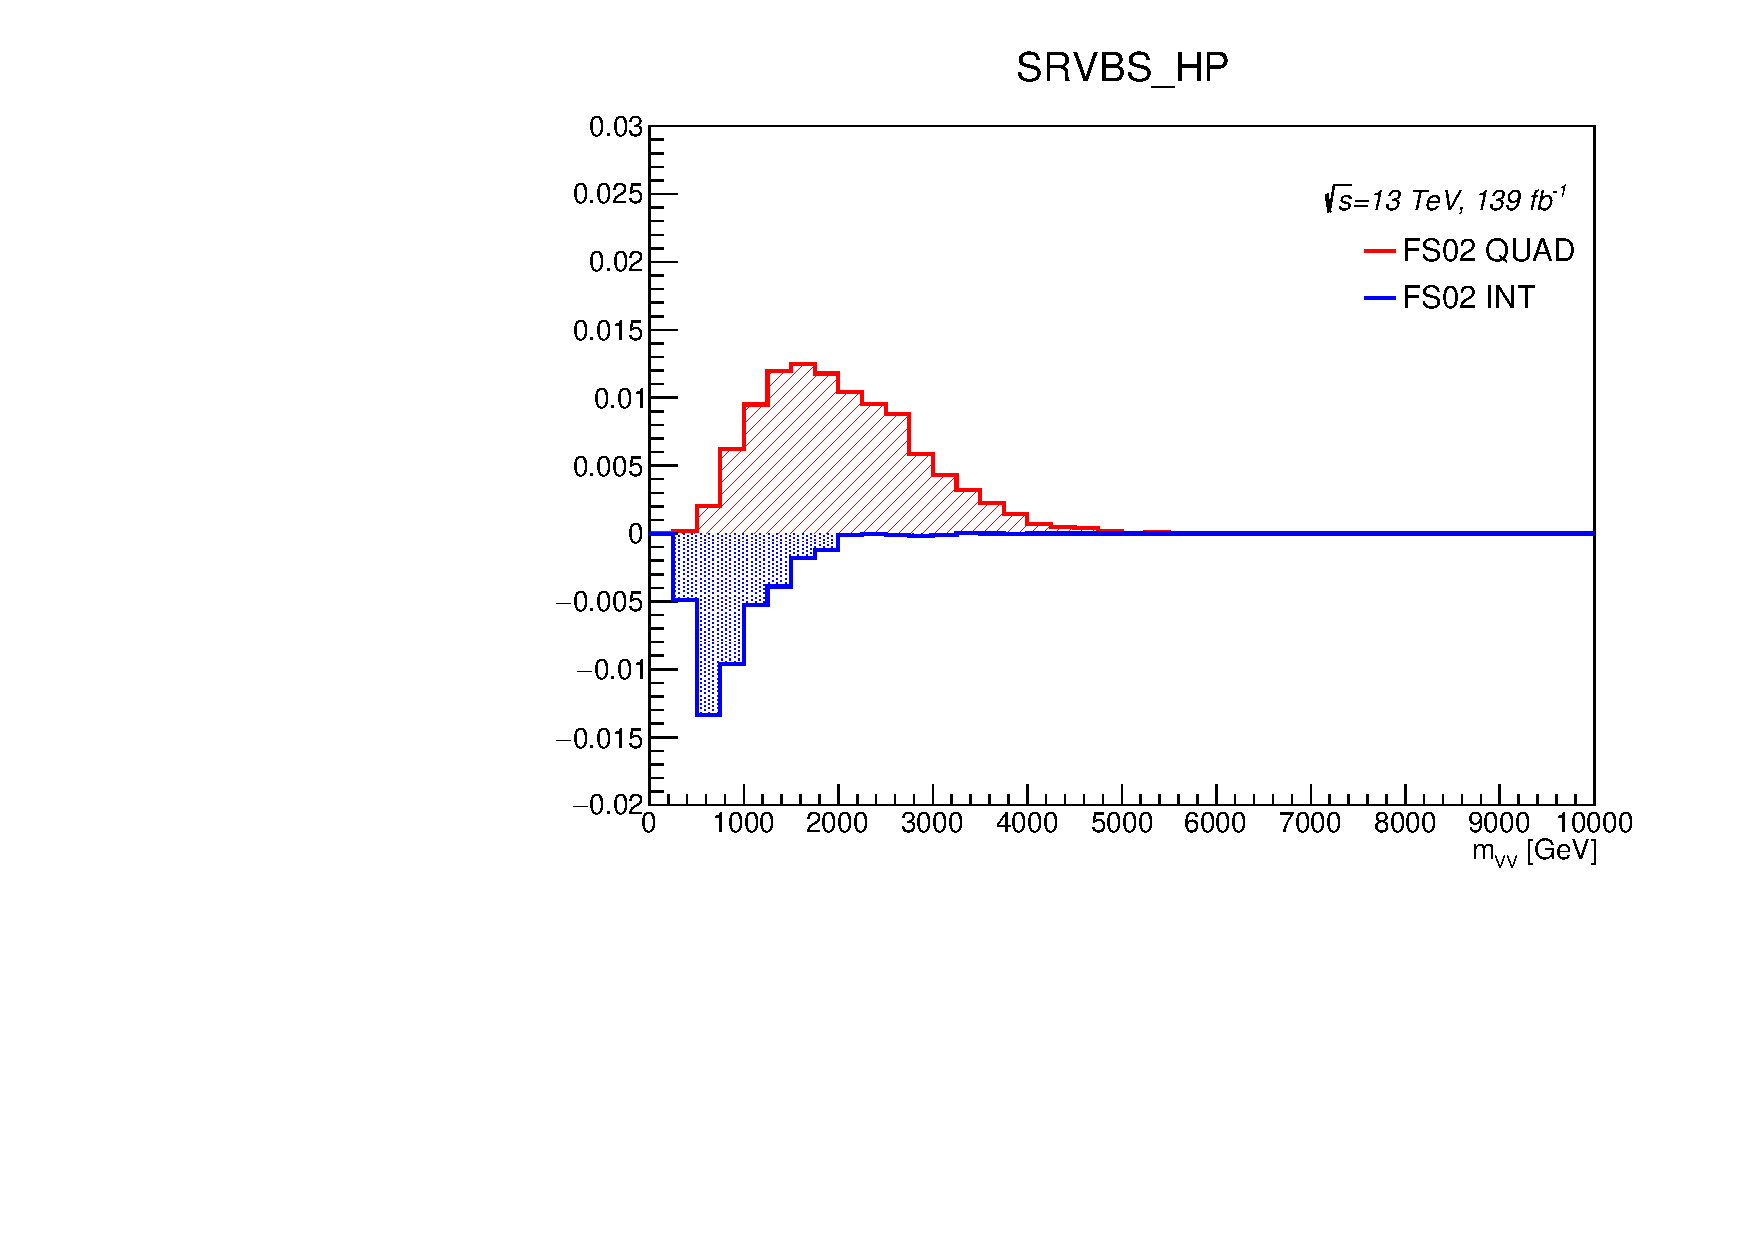
\includegraphics[width=0.45\textwidth]{figures/aQGC/FS02_0ptag1pfat0pjet_0ptv_SRVBS_HP_MllJ.pdf}
        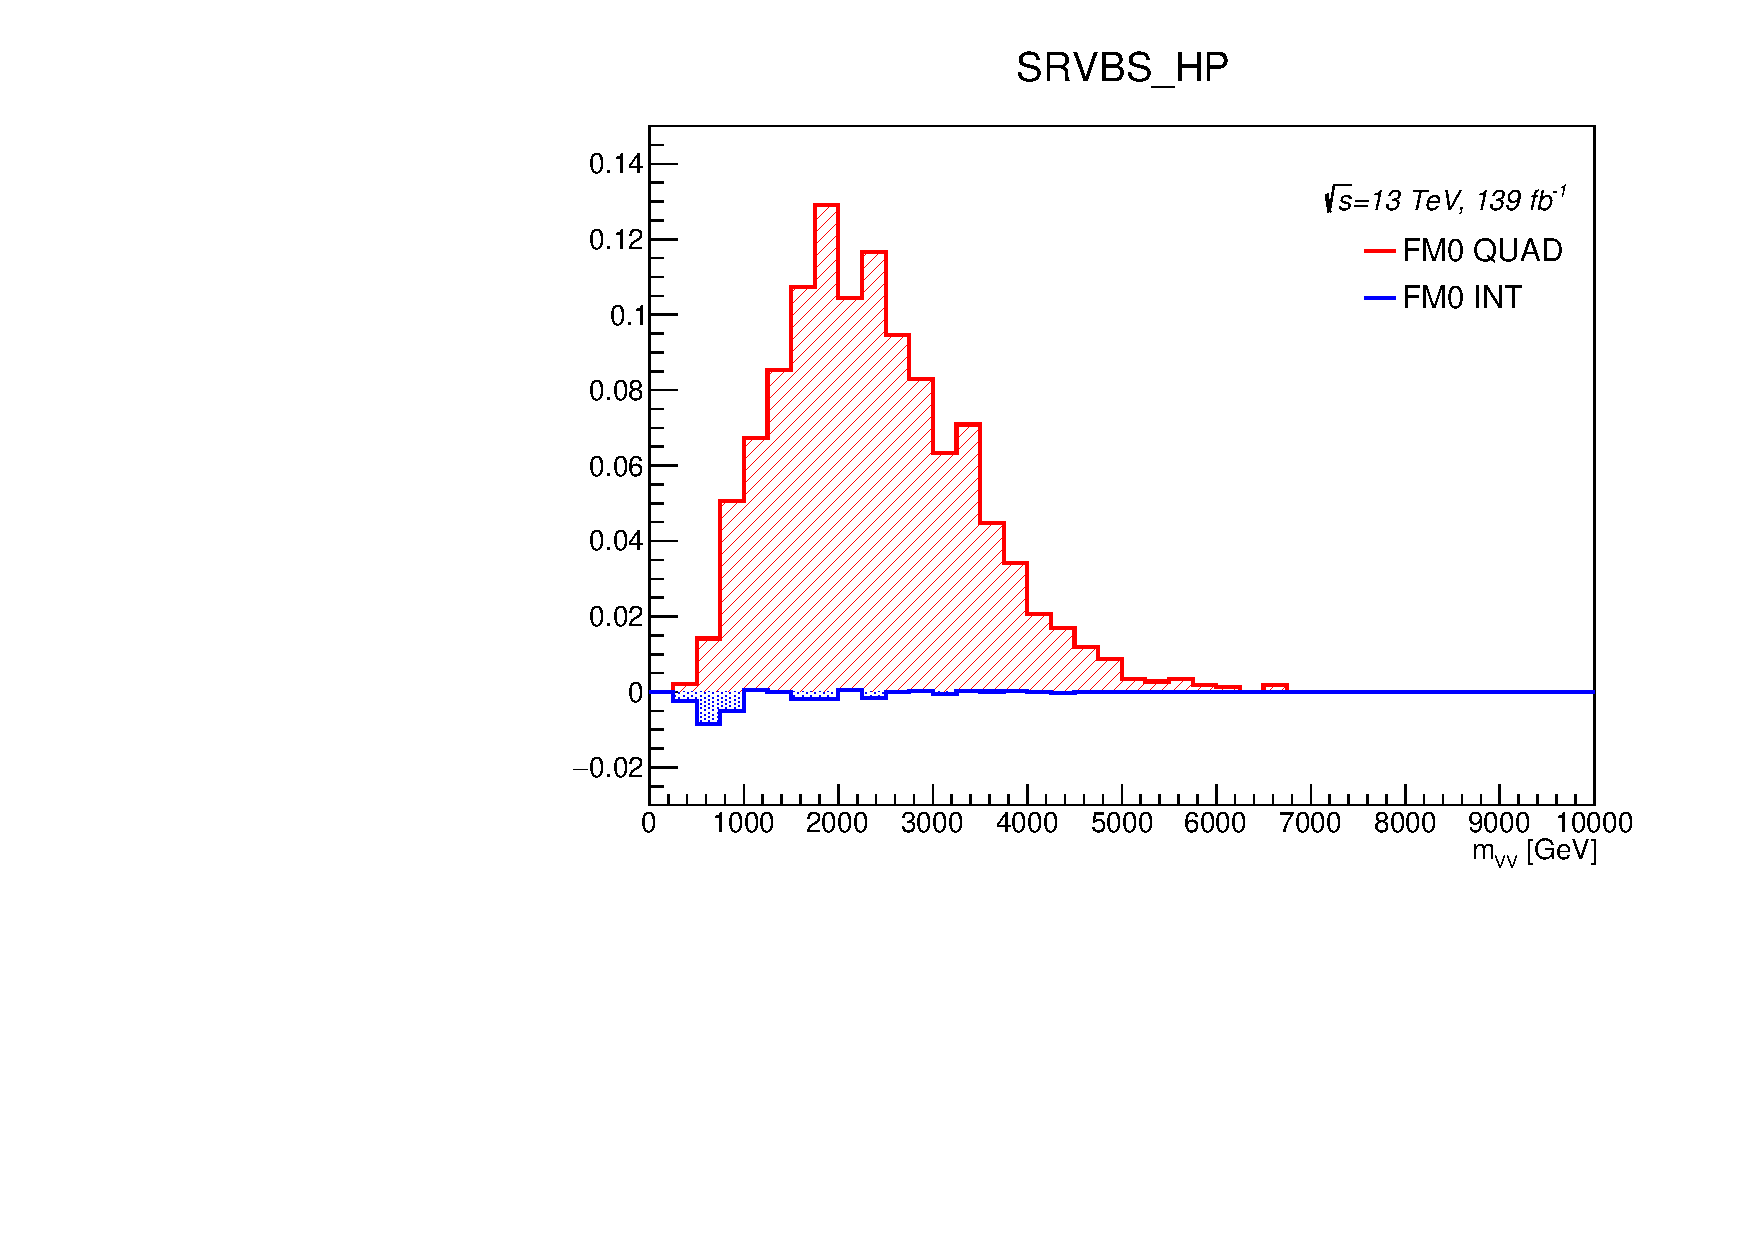
\includegraphics[width=0.45\textwidth]{figures/aQGC/FM0_0ptag1pfat0pjet_0ptv_SRVBS_HP_MllJ.pdf}
        \caption{The comparison of the quadratic term and the interference term with FT0 (top left), FS02 (top right), and FM0 (bottom middle) in 2-lepton channel HP SR. The contribution of the interference term can be negative, and it is larger in FS terms. }
        \label{fig:quadint}
\end{figure}



For purpose of excluding a signal hypothesis, confidence intervals are derived to set limits. 
Confidence intervals are calculated with asymptotic formulae using Wilks' theorem~\cite{10.1214/aoms/1177732360}, assuming that the profile likelihood test statistic is $\chi^2$ distributed~\cite{Cowan:2010js}.

\section{Clipping method}
\label{subsec:clipping}
As the EFT may violate unitarity at large energy scale, the clipping method, mentioned in section~\ref{subsec:EFT}, is used to preserve the unitarity at high center of mass energies. 
The EFT signal is set to zero at truth $m_{VV} > E_{clip}$, where the $E_{clip}$ is [1.5, 2, 3, 5, $\infty$]~TeV. 
%Figure~\ref{fig:clipped} shows how the $m_{VV}$ is shown at the low clipping energy.
The background samples, which is the all standard model predictions, are not clipped.
%5 points are chosen as recommended from the anomalous gauge couplings (aGC) taskforce.~\cite{ATL-COM-PHYS-2017-433} 
5 points are chosen so that we can compare the results with other channels or experiments.
The expected and observed limits are obtained with all 3 channels at each of the clipping points and compared with the theoretical unitarity bound.

\section{Study of final discriminant in aQGC search}
\label{subsec:2binapproach}
The aQGC terms can modify the amplitude of the VBS process at the higher effective center-of-mass energy, 
$m_{VV}$, as shown in Figure~\ref{fig:2lepaQGCshapeMVVh}.
It is found that the reconstructed $m_{VV}$ (or \mt\ in \zlep\ channel) is the best variable to separate the aQGC signals from the background,
while the RNN score distributions for the aQGC samples are similar to the one for the SM electroweak signal and still useful to suppress the non-VBS background as shown in Fig.~\ref{fig:2lepaQGCshapeRNNh}.

\begin{figure}[]
    \centering
   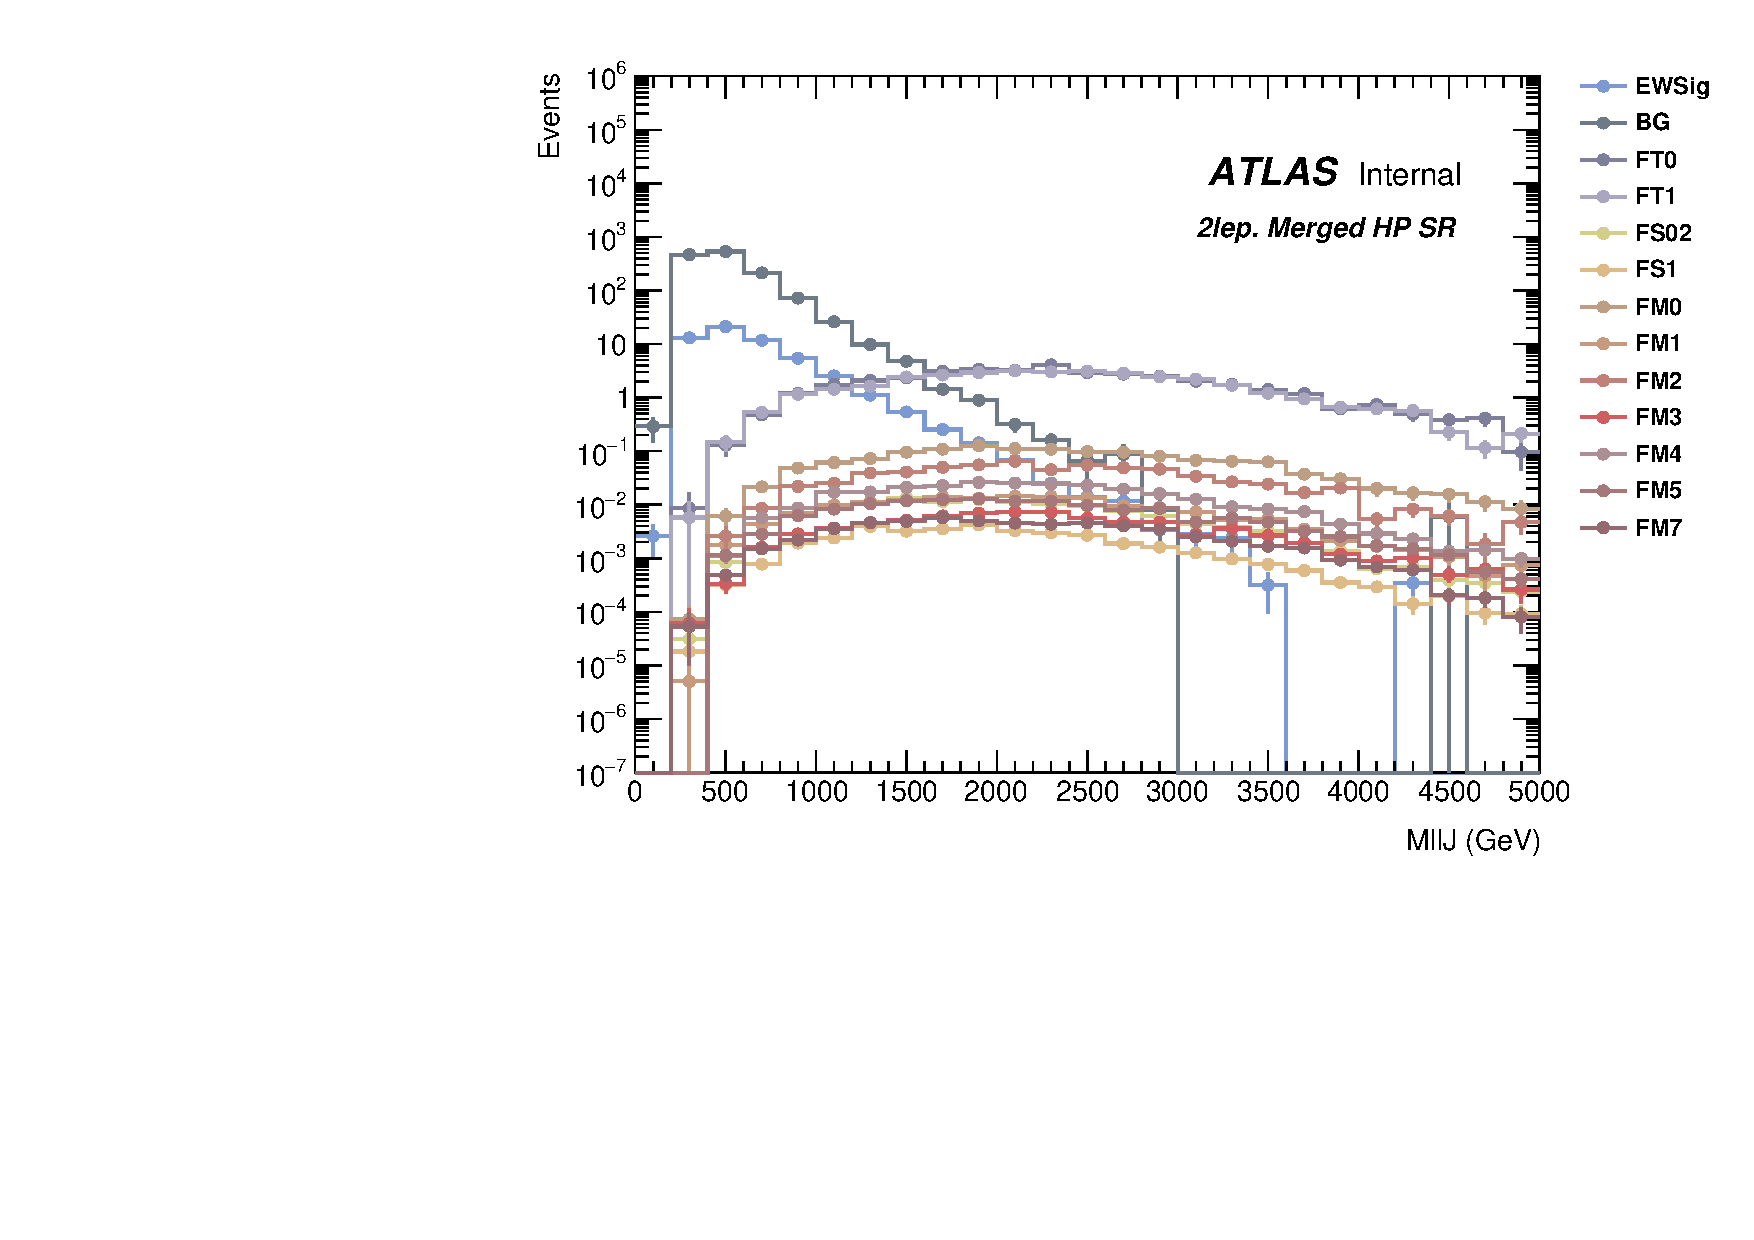
\includegraphics[width=0.45\textwidth]{figures/aQGC/MllJ_SR_HP_aQGC.pdf}
   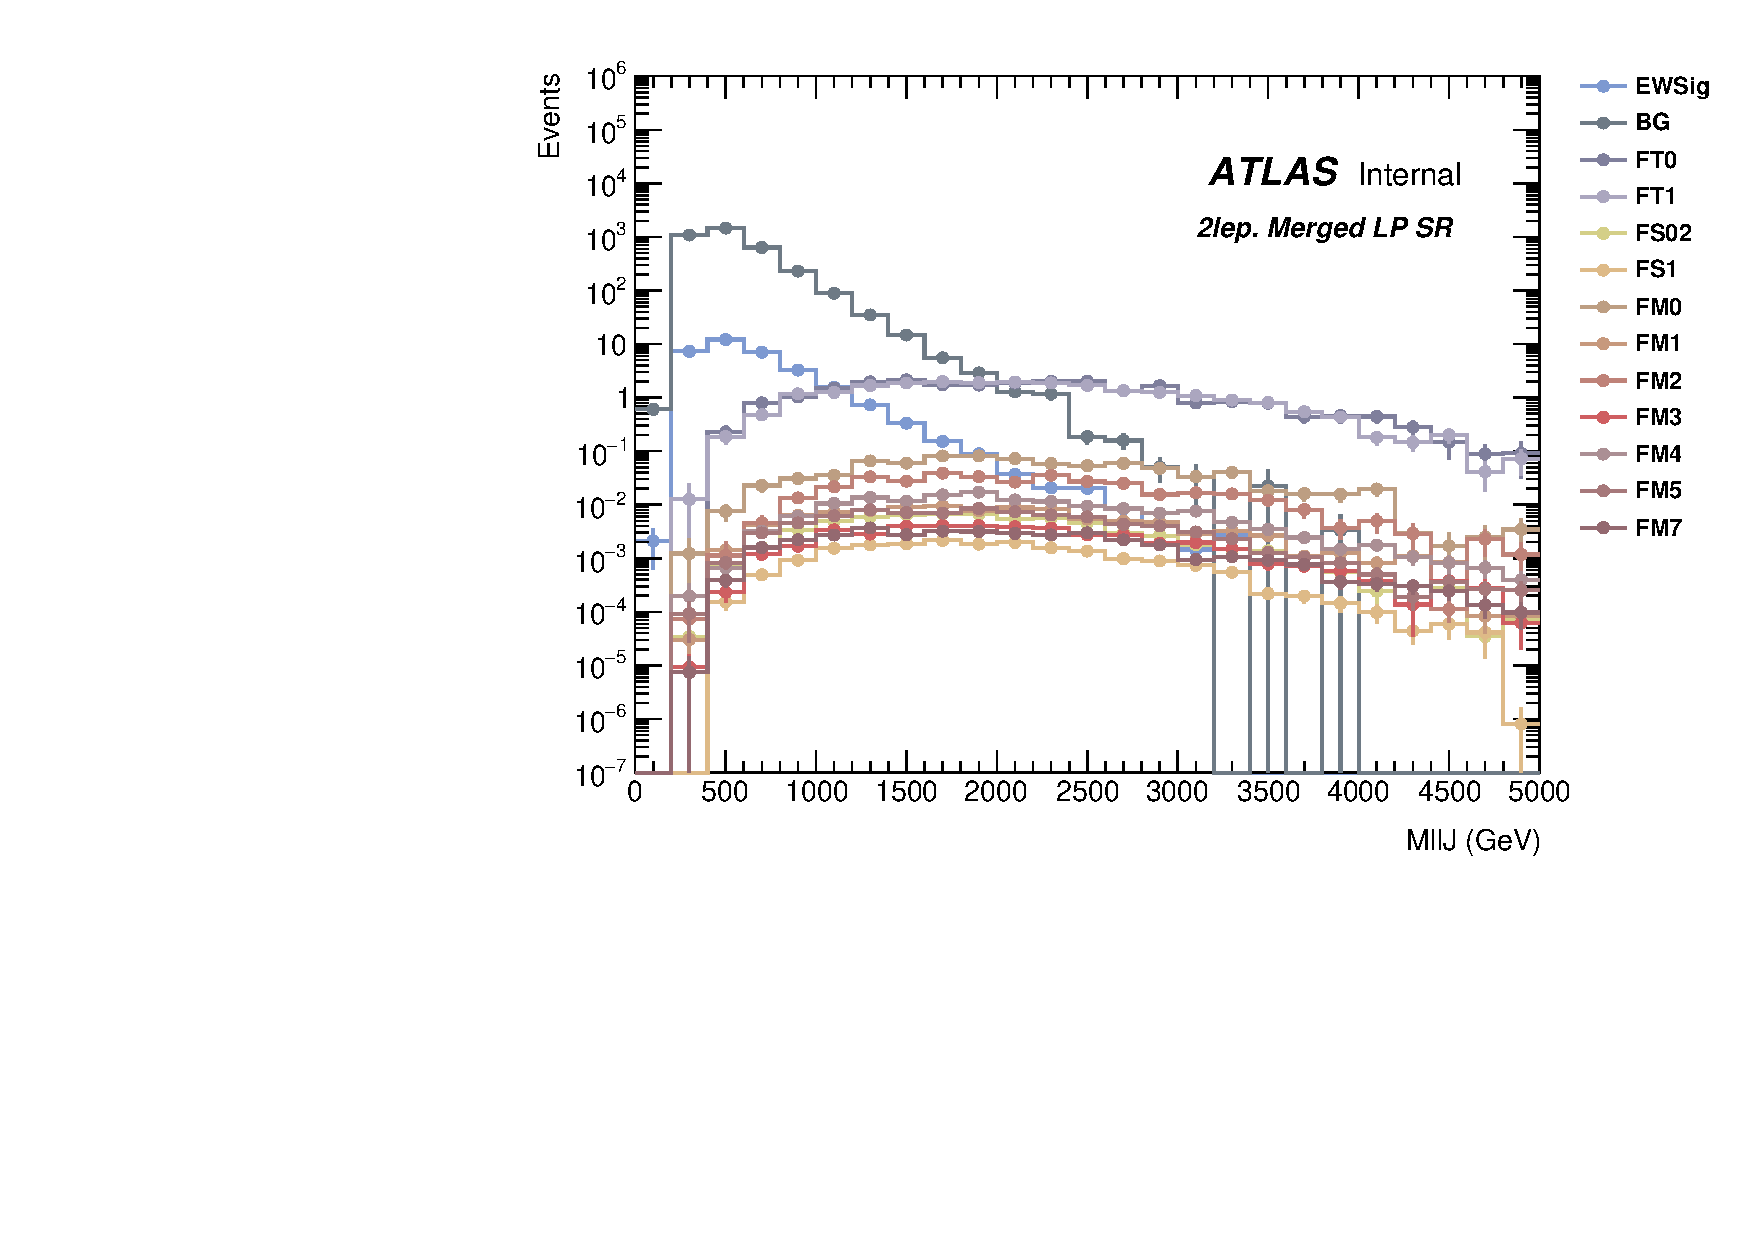
\includegraphics[width=0.45\textwidth]{figures/aQGC/MllJ_SR_LP_aQGC.pdf}
    \caption{$m_{VV}$ shape distribution of each Wilson coefficient in Merged Signal regions. Only quadratic terms are shown.}
    \label{fig:2lepaQGCshapeMVVh}
\end{figure}

\begin{figure}[]
    \centering
   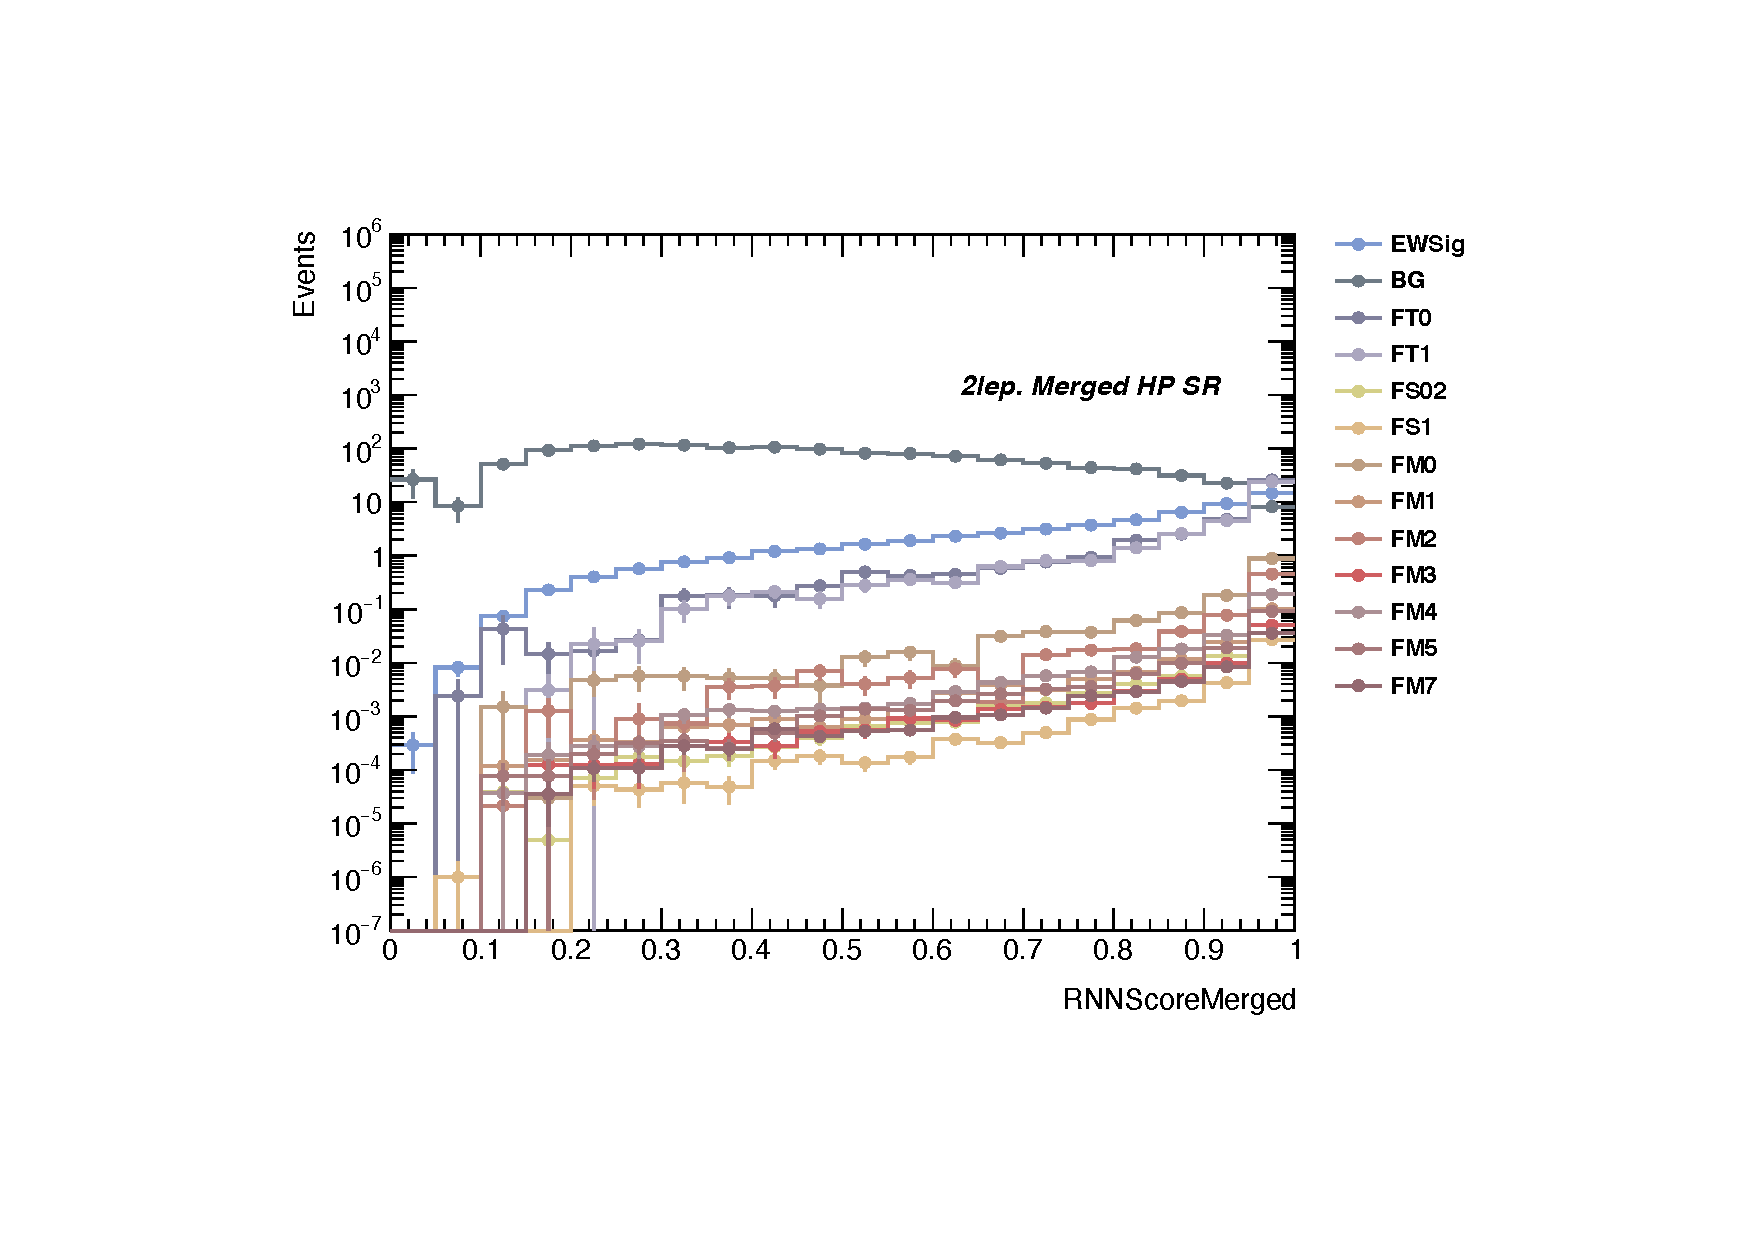
\includegraphics[width=0.45\textwidth]{figures/aQGC/RNNScoreMerged_SR_HP_aQGC.pdf}
   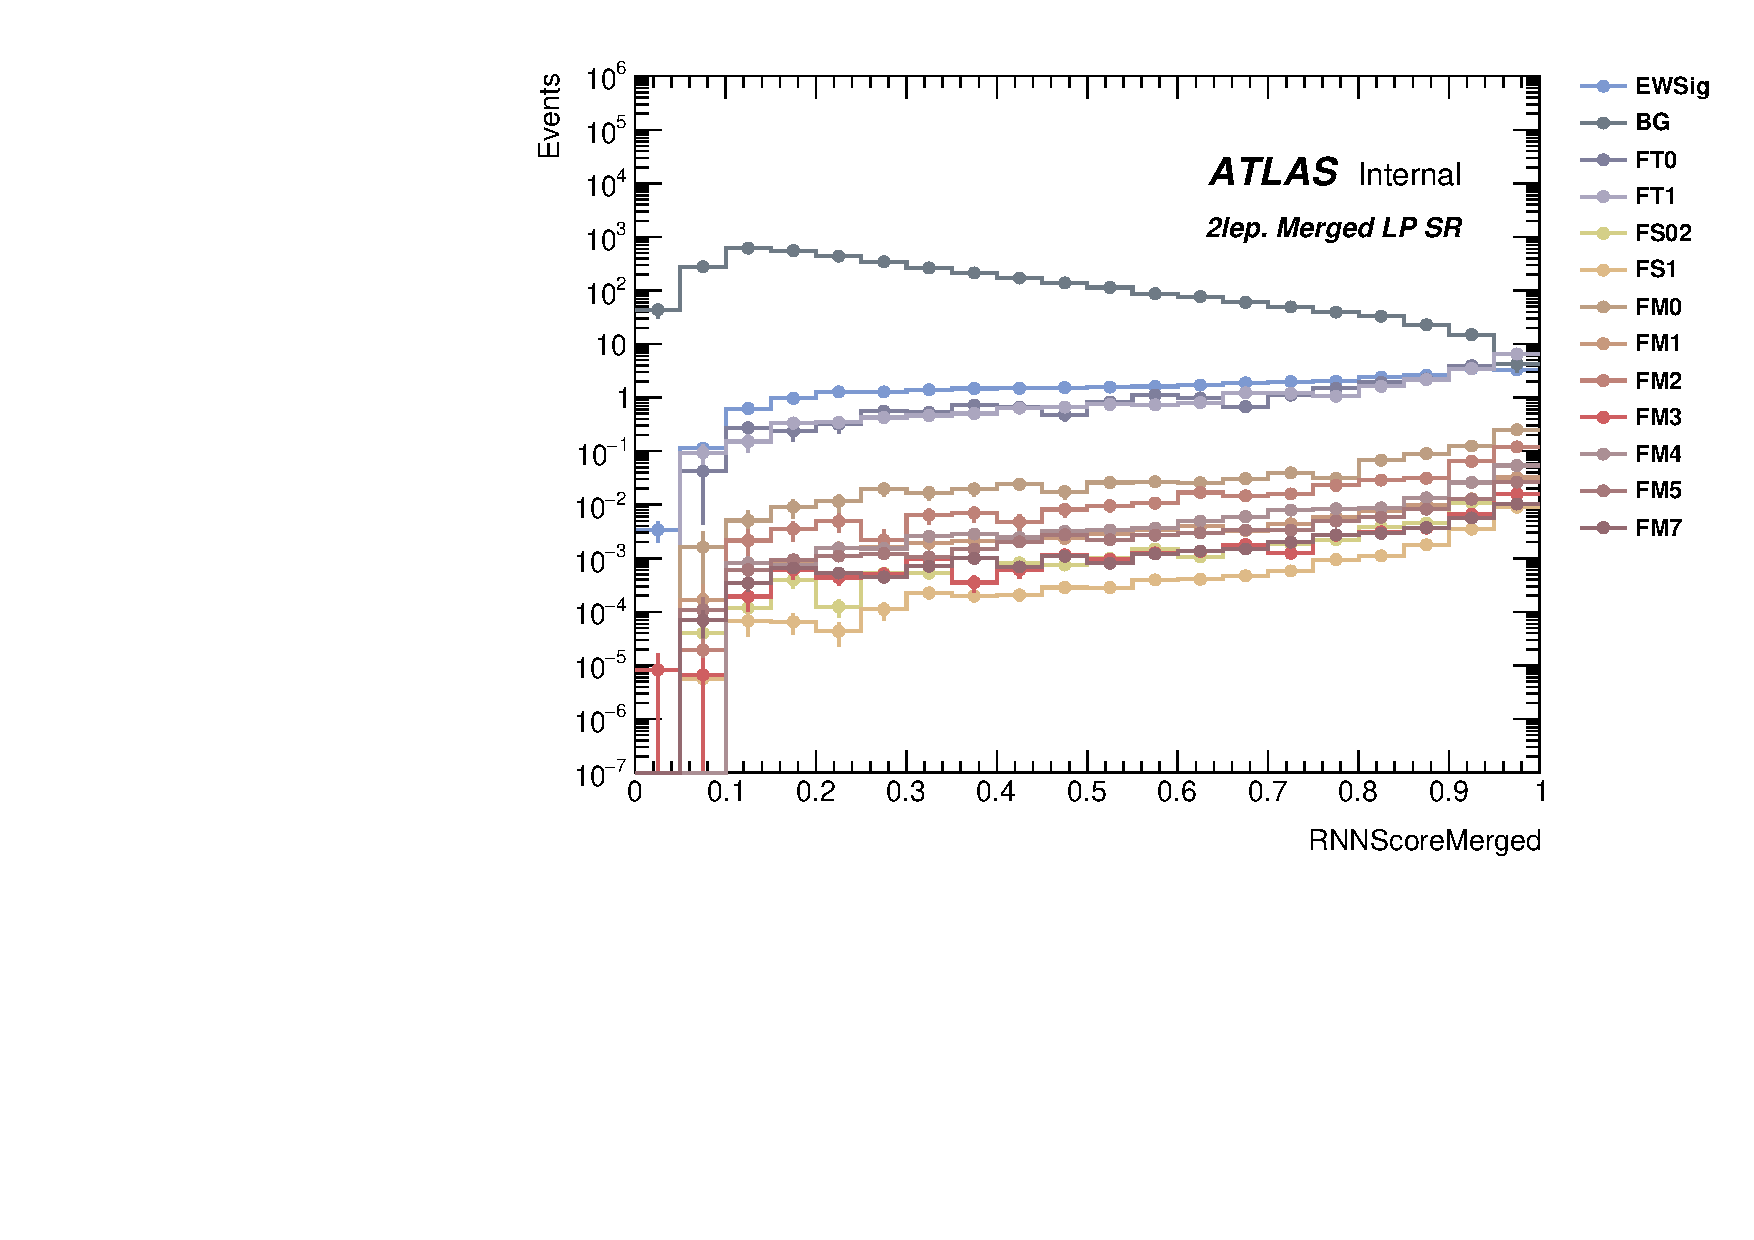
\includegraphics[width=0.45\textwidth]{figures/aQGC/RNNScoreMerged_SR_LP_aQGC.pdf}
    \caption{RNN score shape distribution of each Wilson coefficient in Merged Signal regions. Only quadratic terms are shown.}
    \label{fig:2lepaQGCshapeRNNh}
\end{figure}
%Two-dimensional binning of $m_{VV}$ and the RNN score is used as the final discriminant for the aQGC search.
%In this section, the optimal binning strategy is studied in \tlep\ channel.
%To confirm the result in Section~\ref{subsec:binnedsig} with more realistic setting,

Finally, we would like to separate aQGC signals from both SM electroweak signal and the SM non-VBS background.
So that the final discriminant can make use of the both separation power of $m_{VV}$ and the RNN score, the following study has been performed.

%we compared the results with the following conditions.
The fitting results with the following conditions are compared:
\begin{itemize}
  \item A fit to $m_{VV}$ distribution as discriminant, without any cuts on the RNN score;
  \item A fit to the RNN score distributions after
        SRs are further separated into two subcategories: \\
        Low $m_{VV}$ : $m_{VV}$ $< 2000$~GeV and \\
        High $m_{VV}$ : $m_{VV}$ $\geq 2000$~GeV. \\
\end{itemize}
The threshold 2000~GeV is derived from figure~\ref{fig:2lepaQGCshapeMVVh}.
With the second option, the number of SRs is twice as shown in Figure~\ref{fig:2lepTwoBin}.
%(binning??)
Unconditional asimov fit (The log-likelihood fit using asimov dataset without fixing the $\mu$ value) by using FT0 signal in only \tlep\ channel is performed.
Only quadratic term is used in this study.
The systematic uncertainties are not included in the fitting here, just the floated normalization factor is considered.
The asimov data used here is constructed from the background plus SM electroweak VV+jj signal samples.
The expected limits and uncertainty of the expected signal strength of FT0 signal are shown in table~\ref{tab:2binlimit}.
%Significantly better upper limit on the signal strength is obtained by the second option (a fit to RNN score with the categorization by $m_{VV}$)
%than the first option (a fit to $m_{VV}$ distribution).
The signal strength obtained by the second option (a fit to RNN score with the categorization by $m_{VV}$) and the first option (a fit to $m_{VV}$ distribution) is the same. 
We found the first option cannot give any constraints on the SM electroweak VV+jj signal.
It can be a motivation to use the RNN score also in the aQGC search study.

\begin{figure}[ht]
    \centering
    	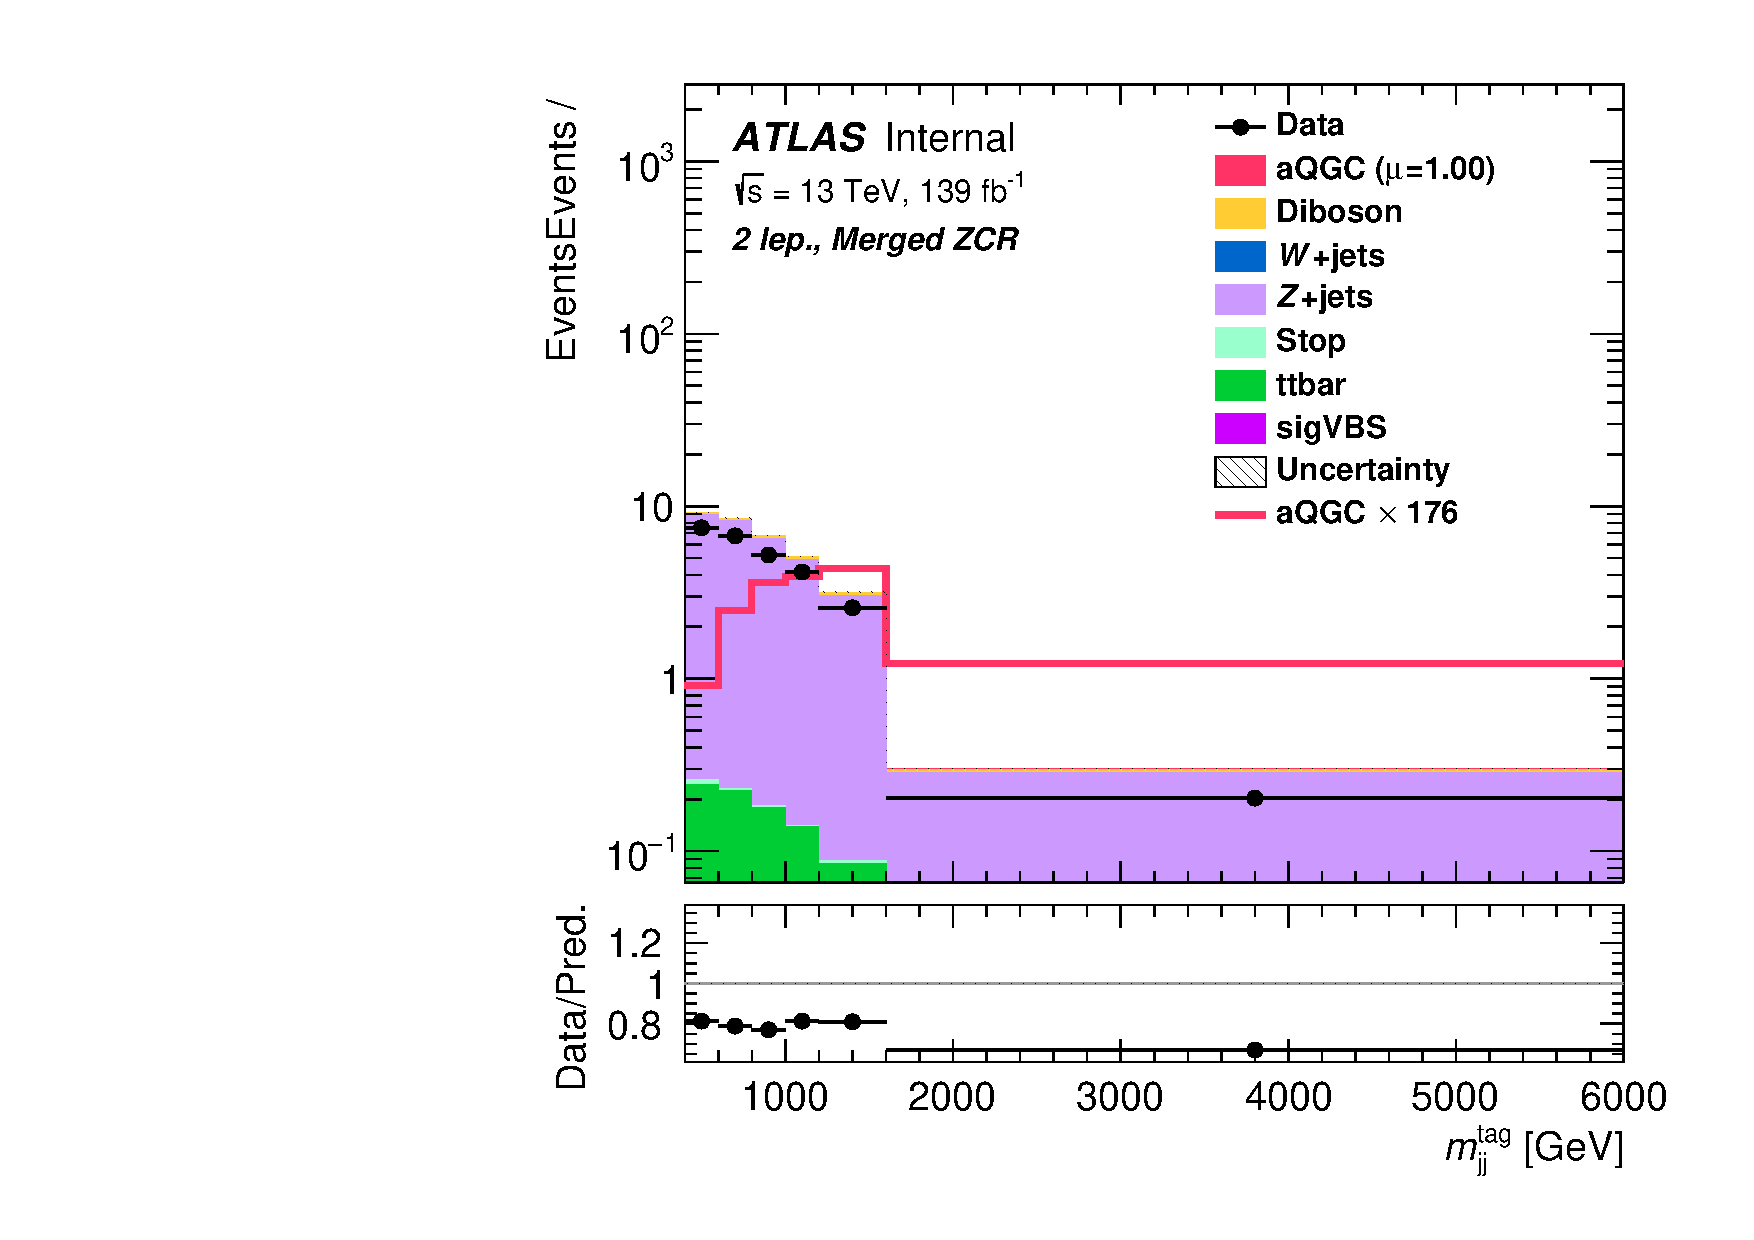
\includegraphics[width=0.32\textwidth]{figures/aQGC/Region_distMTagMerJets_DCRVjet_BMin0_J0_incJet1_L2_T0_incFat1_Y6051_incTag1_Fat1_Prefitlog.pdf}
    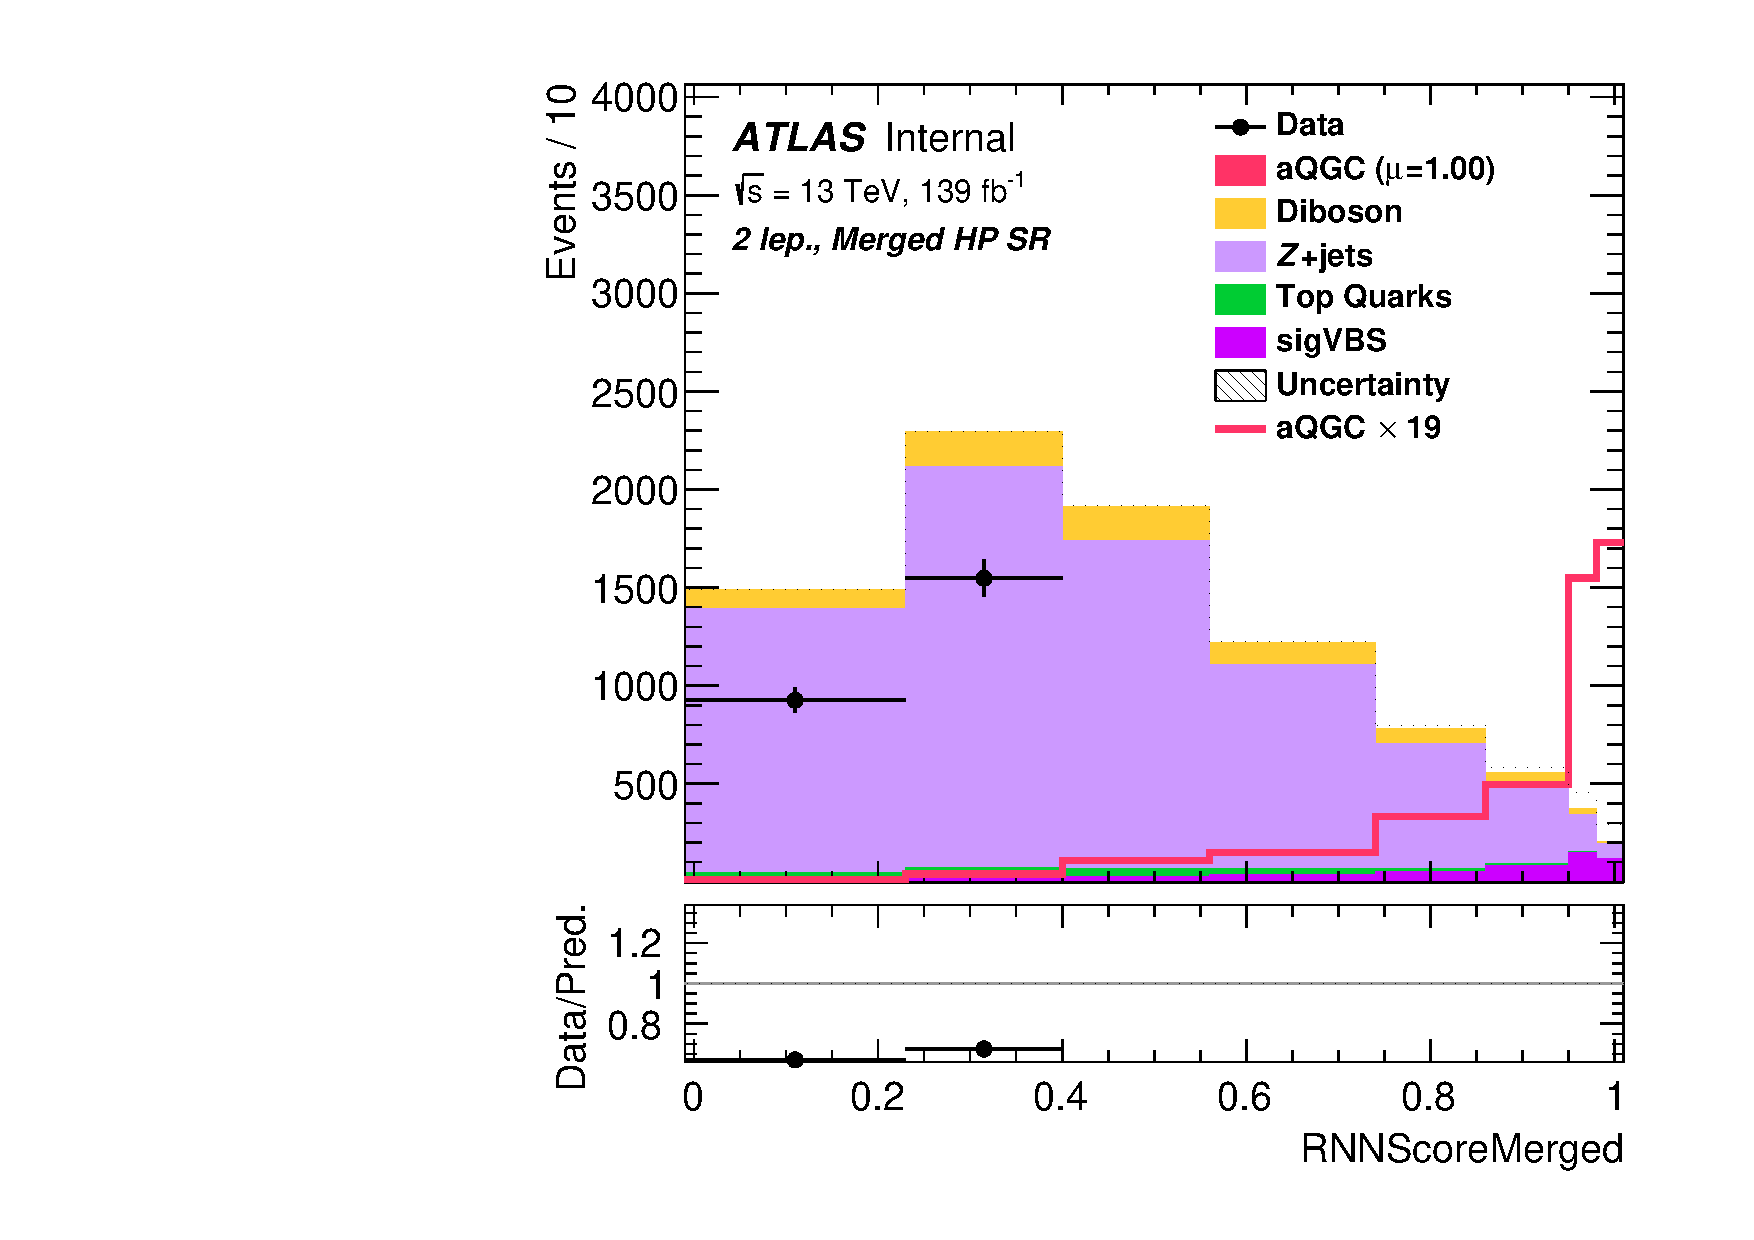
\includegraphics[width=0.32\textwidth]{figures/aQGC/Region_distRNNScoreMerged_DSRVBSHPLMVV_BMin0_J0_incJet1_L2_T0_incFat1_Y6051_incTag1_Fat1_Prefit.pdf}
 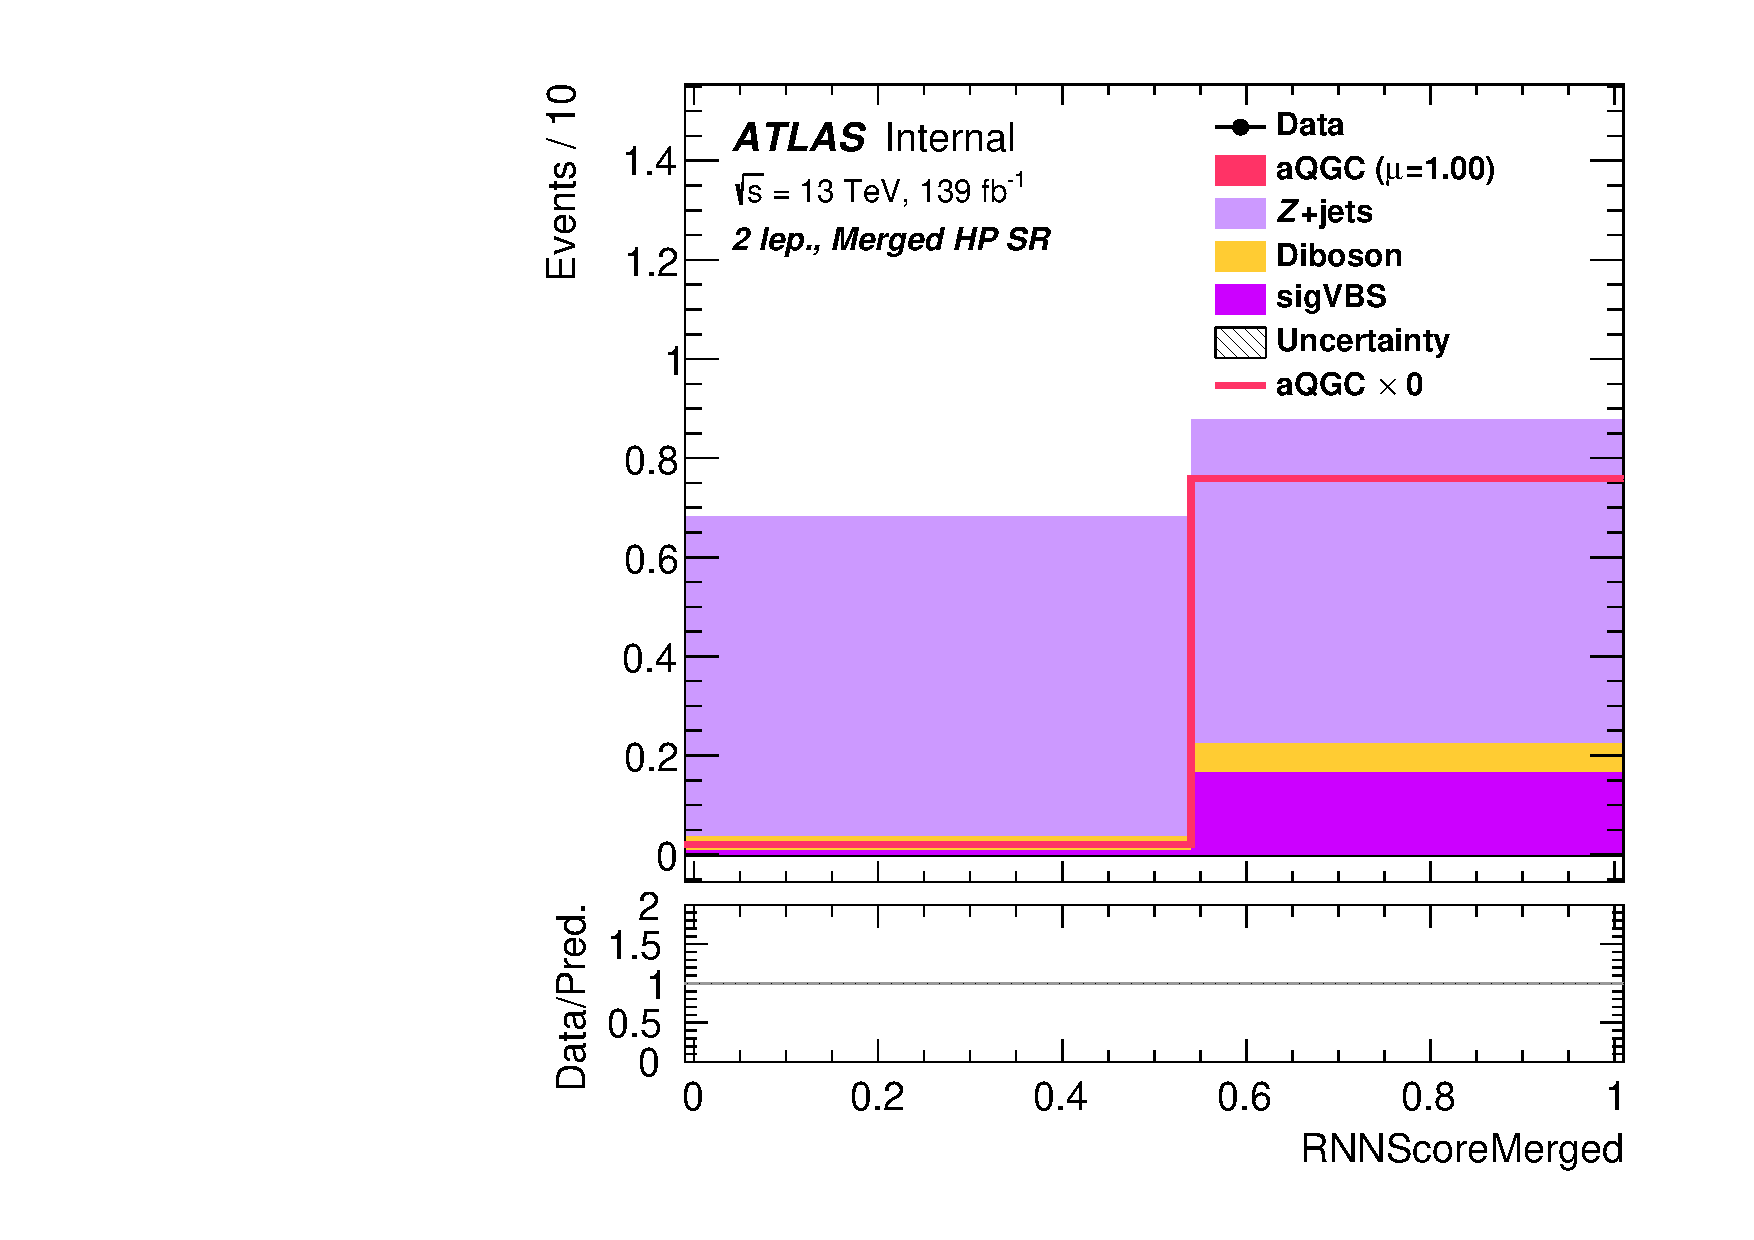
\includegraphics[width=0.32\textwidth]{figures/aQGC/Region_distRNNScoreMerged_DSRVBSHPHMVV_BMin0_J0_incJet1_L2_T0_incFat1_Y6051_incTag1_Fat1_Prefit.pdf}
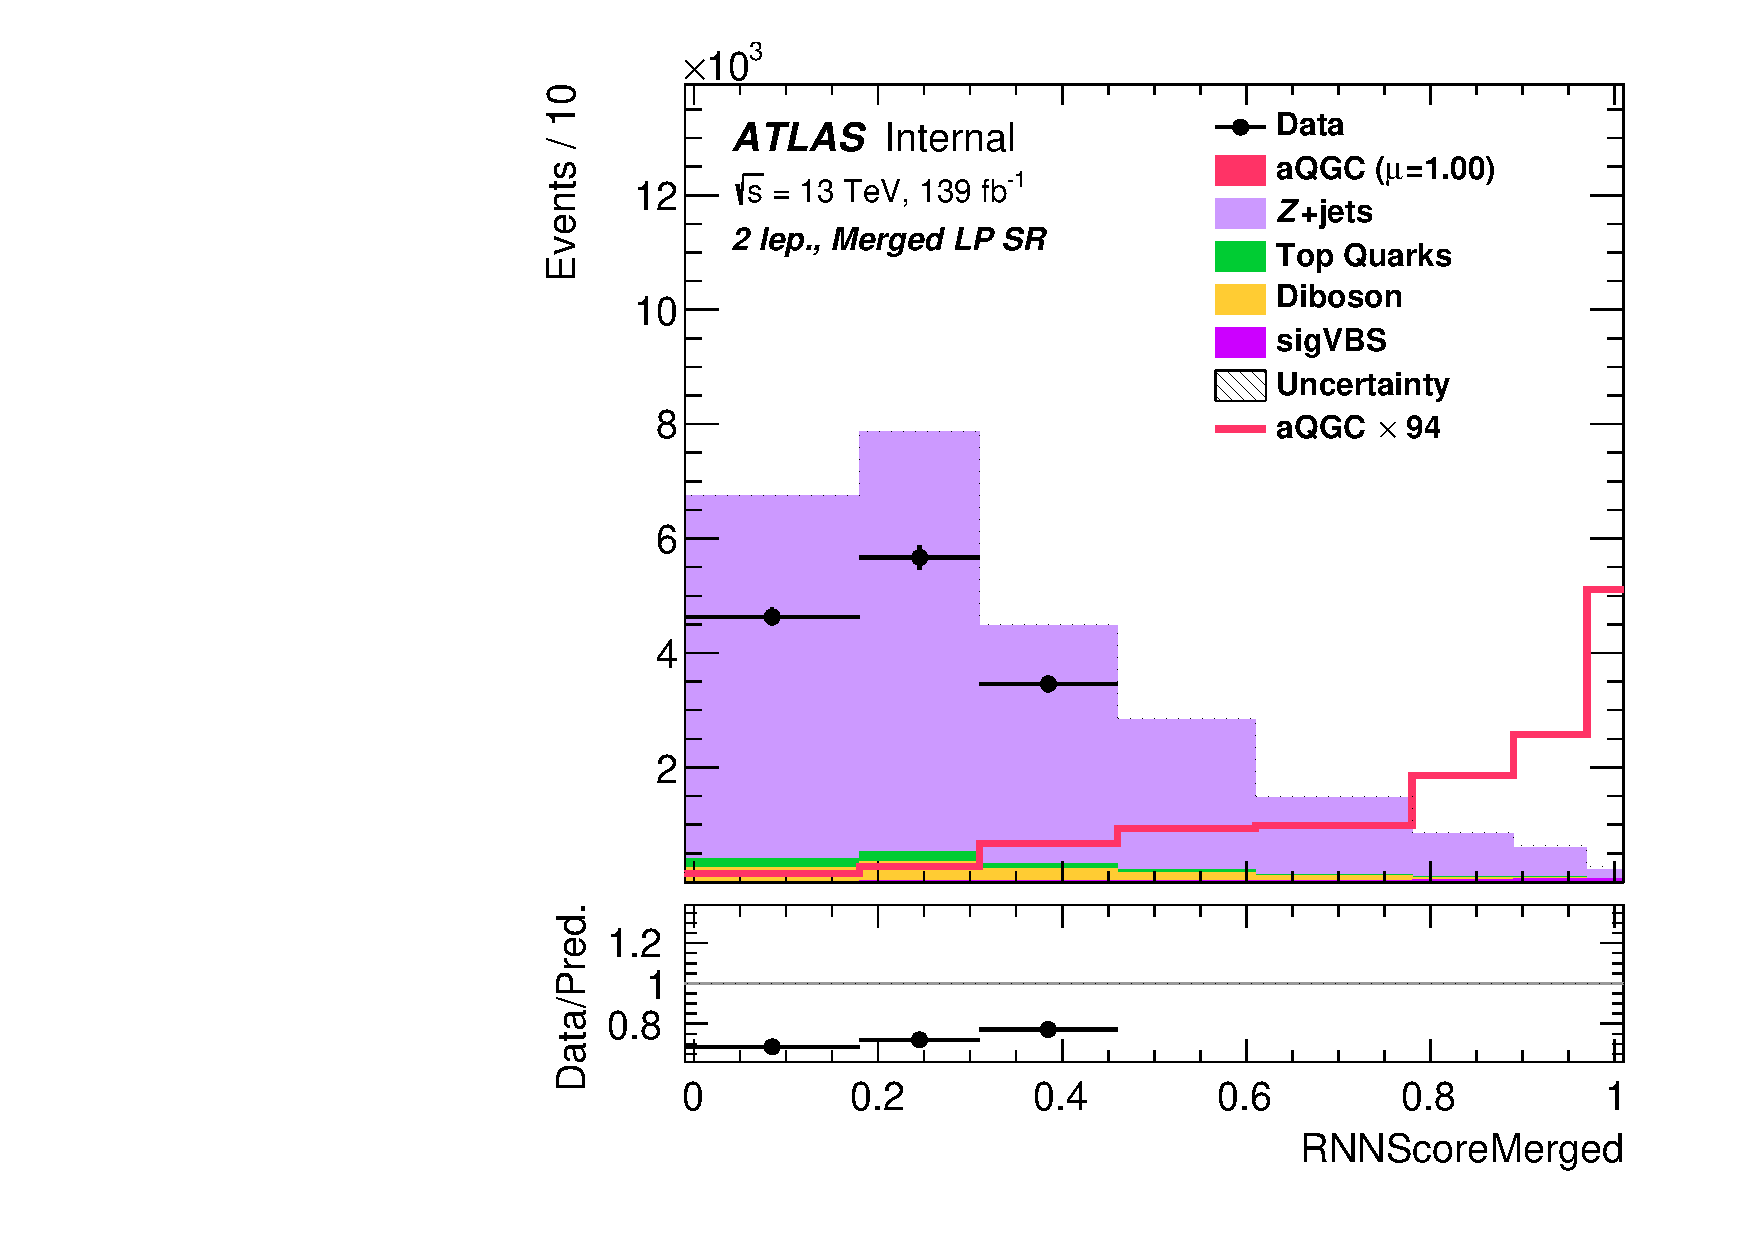
\includegraphics[width=0.32\textwidth]{figures/aQGC/Region_distRNNScoreMerged_DSRVBSLPLMVV_BMin0_J0_incJet1_L2_T0_incFat1_Y6051_incTag1_Fat1_Prefit.pdf}
    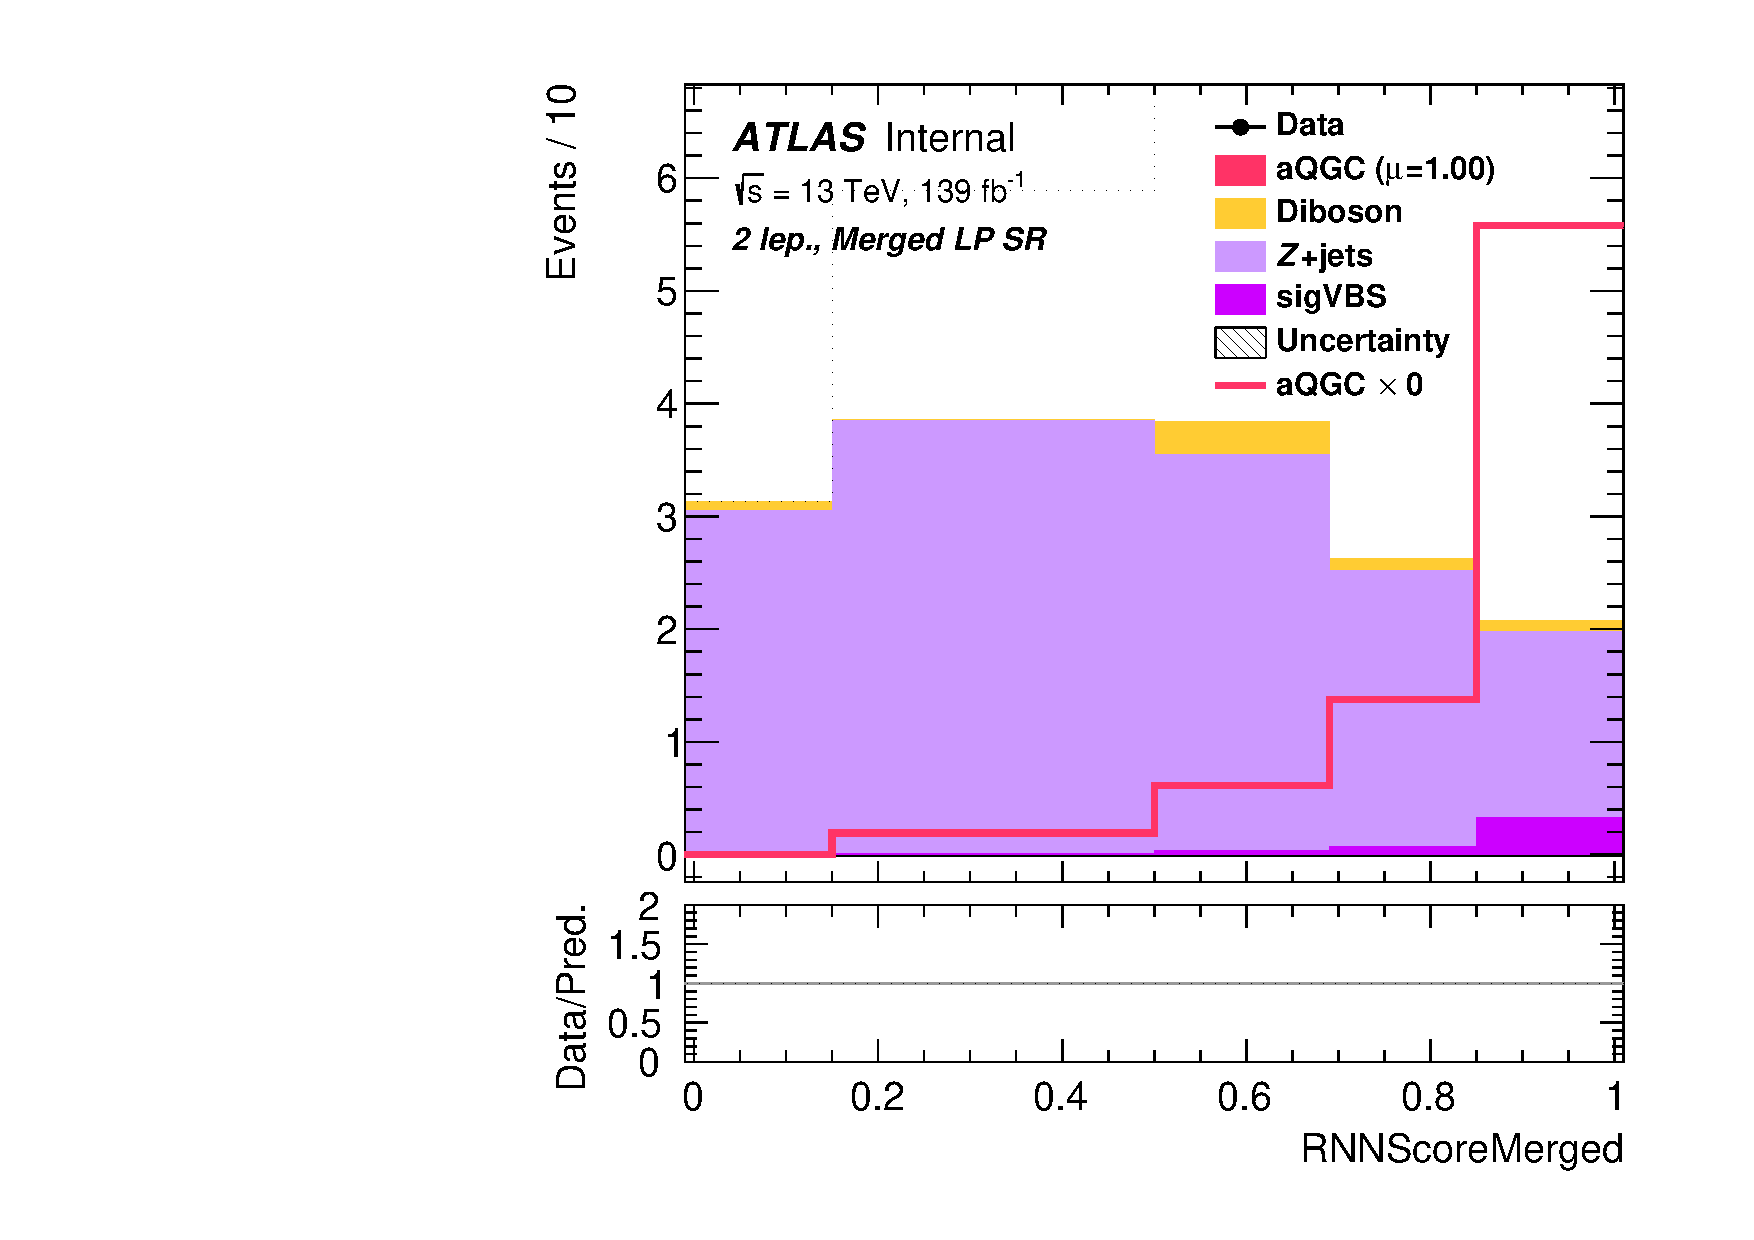
\includegraphics[width=0.32\textwidth]{figures/aQGC/Region_distRNNScoreMerged_DSRVBSLPHMVV_BMin0_J0_incJet1_L2_T0_incFat1_Y6051_incTag1_Fat1_Prefit.pdf}
        \caption{Prefit plots for 2-bin strategy are shown. The RNN score is used as a discriminant for signal regions. operator FT0 in \tlep\ channel are shown. The standard model EW signal is floated as the background.}
        \label{fig:2lepTwoBin}
\end{figure}

%\begin{table}[ht!]
%\small
%\begin{center}
%\resizebox{0.9\textwidth}{!}{
%\begin{tabular}{ | l || l | l | l |}
%\hline
%                                    & Fit to $m_{VV}$ w/o further categorization & Fit to RNN score w/o further categorization  & Fit to RNN scores in separated bins of low- and high-$m_{VV}$  \tabularnewline \hline
%Unconditional fitted $\mu$          & -2.7e-06 $\pm$ 0.067   & 3.38e-05 $\pm0.038$      & 3.35e-05 $\pm0.029$  \tabularnewline \hline
%Norm sigVBS                         & 1 $\pm$ 2.1            & 1 $\pm$ 0.94             & 1 $\pm$ 0.48         \tabularnewline \hline
%Norm Z                              & 1 $\pm$ 0.036          & 1 $\pm$ 0.029            & 1 $\pm$ 0.027        \tabularnewline \hline
%Norm VV                             & 1 $\pm$ 1.13           & 1 $\pm$ 0.71             & 0.99 $\pm$ 0.64      \tabularnewline \hline
%Expected limit of $\mu$             & 0.19                   & 0.72                     & 0.10                 \tabularnewline \hline
%Expected limit of Wilson coefficient & 0.44                   & 0.85                     & 0.32                 \tabularnewline \hline
%\end{tabular}
%}
%\caption{Expected signal strength and limits in every two options. only \tlep channel is used for the fit. The result for single bin fit with RNN is also shown as a reference. The normalization fitted for standard model signal, and Z and diboson backgrounds are shown as Norm in the table.}
%\label{tab:2binlimit}
%\end{center}
%\end{table}

\begin{table}[ht!]
\small
\begin{center}
\resizebox{\textwidth}{!}{
\begin{tabular}{ | l || l | l | l |}
\hline
                                    & Fit to $m_{VV}$ w/o further categorization & Fit to RNN score w/o further categorization  & Fit to RNN scores in separated bins of low- and high-$m_{VV}$  \tabularnewline \hline
Unconditional fitted $\mu$          & 8.83e-06 $\pm0.032$    & 1.02e-04 $\pm0.34$       & 1.09e-05 $\pm0.028$  \tabularnewline \hline
Norm sigVBS                         & 1 $\pm$ 1.08           & 1 $\pm$ 0.79             & 1 $\pm$ 0.41         \tabularnewline \hline
Norm Z                              & 1 $\pm$ 0.012          & 1 $\pm$ 0.010            & 1 $\pm$ 0.01         \tabularnewline \hline
Expected limit of $\mu$             & 0.11                   & 0.70                     & 0.11                 \tabularnewline \hline
Expected limit of Wilson coefficient & 0.33                  & 0.84                     & 0.33                 \tabularnewline \hline
\end{tabular}
}
\caption{Expected signal strength and limits in every two options. only \tlep~channel is used for the fit. The result for single bin fit with RNN is also shown as a reference. The normalization fitted for the standard model signal, and Z backgrounds are shown as Norm in the table.}
\label{tab:2binlimit}
\end{center}
\end{table}

%\section{Optimization of the threshold of 2-bin approach}
%\label{subsec:aQGCbinninb}
Of course, the optimal threshold of $m_{VV}$ can be different depending on the clipping energy.
In addition, a fine-tuning of the $m_{VV}$ threshold might be needed by considering the stability of the background estimation.
The expected limit is shown in each threshold for $m_{VV}$ of 1000~GeV, 1500~GeV, 2000~GeV for variety of the clipping points in Figure~\ref{fig:ThresholdScan}.

As expected, higher $m_{VV}$ threshold is preferred at the higher clipping point, while lower $m_{VV}$ threshold is favored at the lower clipping point.
1500~GeV is chosen as the best compromise to separate SRs into low- and high-$m_{VV}$ bins.

Since the meaning of the actual $m_{VV}$ distributions used in each lepton channel are different
(fully reconstructed system in \tlep\ and in \olep\ (solving neutrino ambiguity) and transverse mass in \zlep\)
the optimal thresholds to separate SRs into low- and high-$m_{VV}$ bins in \olep\ and \zlep\ channels 
are determined as follows.
In \olep\ channel, the same threshold as \tlep\ channel, 1500~GeV, is just chosen since the reconstructed $m_{VV}$ distribution is similar. 
%(?)
In \zlep\ channel, the threshold needs to be optimized, since it uses \mt\ instead of $m_{VV}$.
As shown in Figure~\ref{fig:mVVdist} the \mt\ shape in \zlep\ channel is different from $m_{VV}$ in \tlep\ channel.
Here, the background yield in each bin of the high-$\mt$ regions is adjusted to be more than 5 so that
the asymptotic calculation of the sensitivity is ensured with a certain number of background events.
The threshold finalized is shown in Table, for each lepton channel, and for each region.

Only in \tlep\ channel,
less than 5 background events are expected in the second bin of the HP signal region.
%We are going to test if the asymptotic formulae works fine, by running toy experiments [TO DO].
%
\begin{figure}[h]
        \centering
    	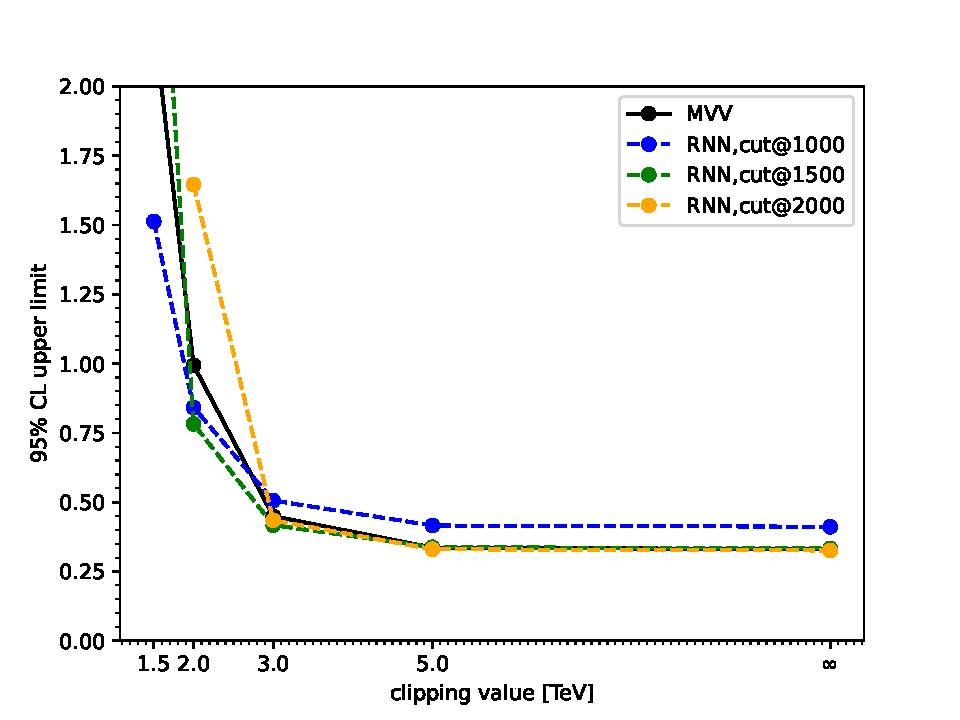
\includegraphics[width=0.50\textwidth]{figures/aQGC/ClippedFT02bin.pdf}
        \caption{Expected limits for 5 clipping points with each threshold for dividing $m_{VV}$ into 2 bins.}
        \label{fig:ThresholdScan}
\end{figure}

\begin{figure}[ht]
    \centering
    	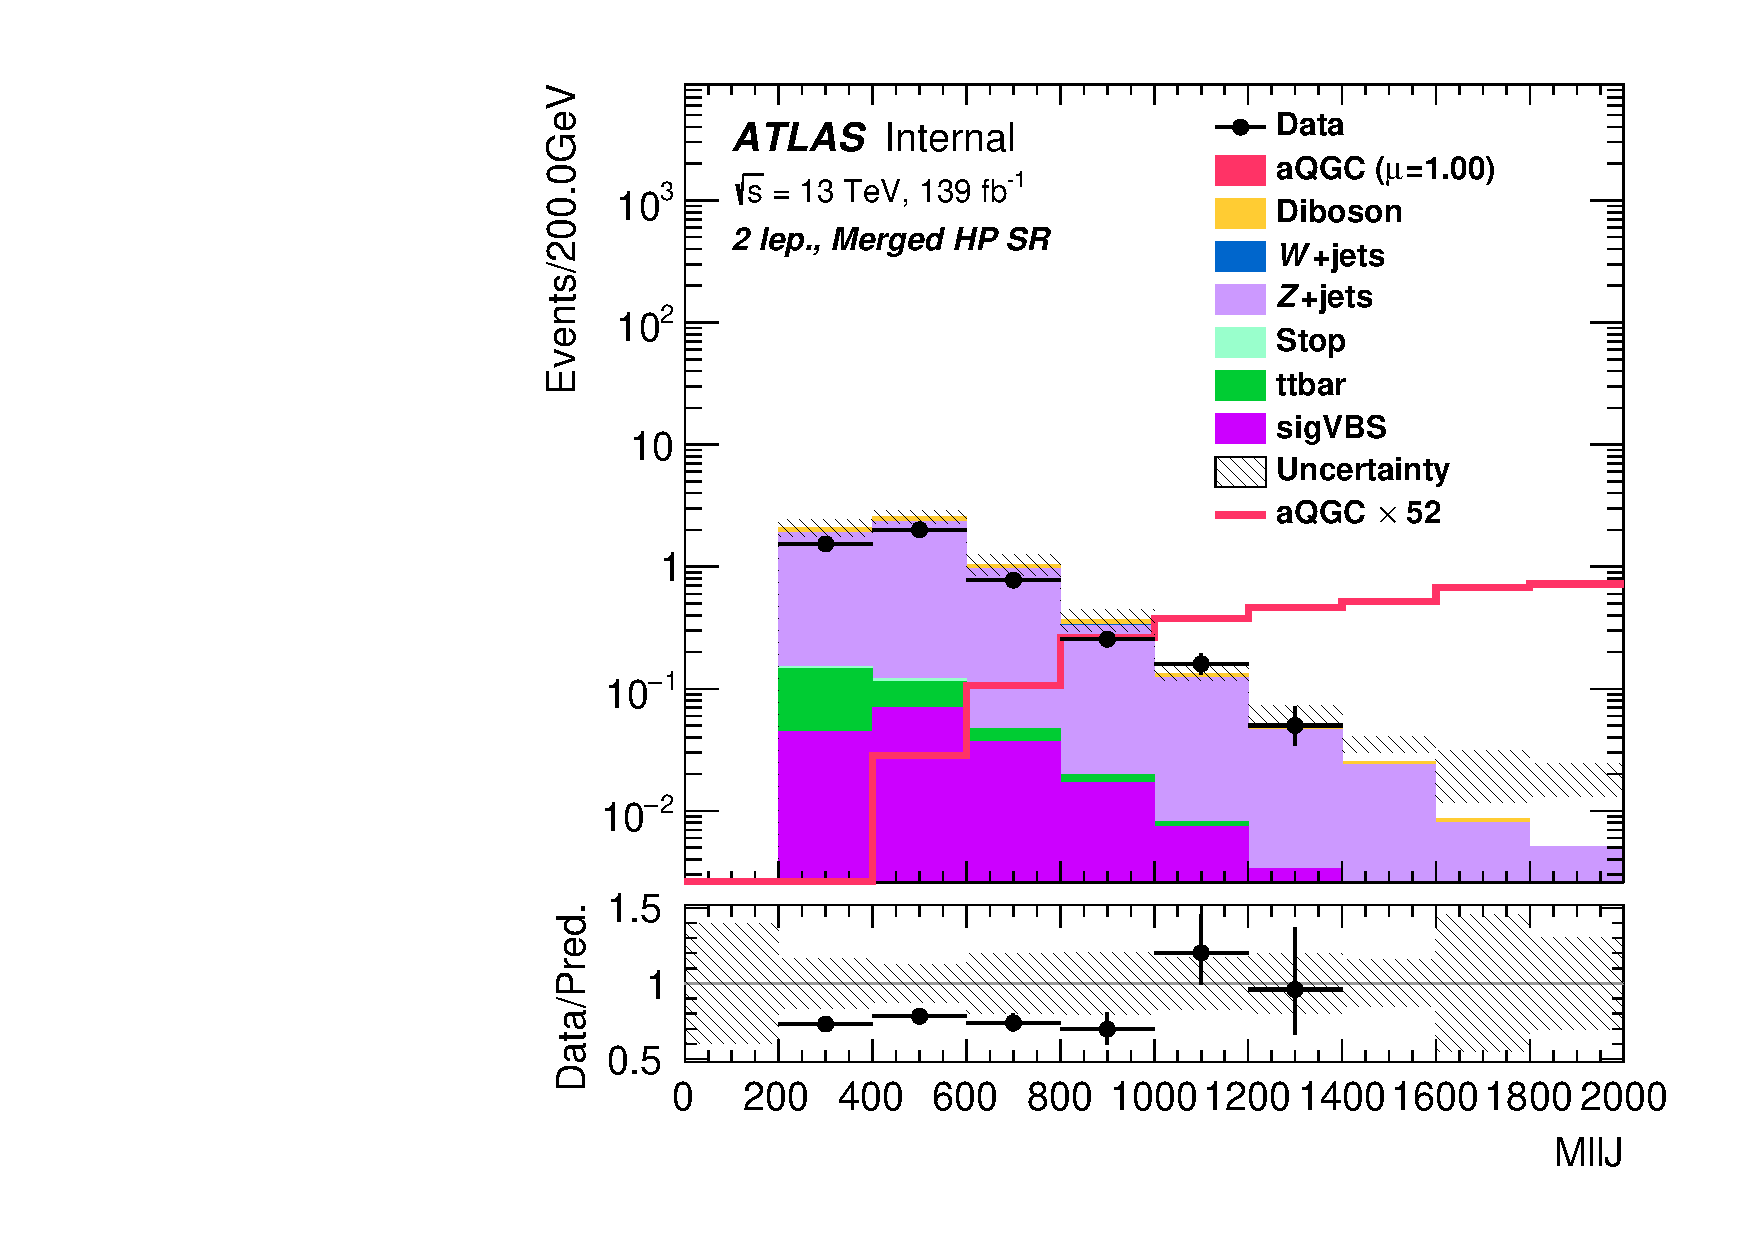
\includegraphics[width=0.32\textwidth]{figures/aQGC/MVV/Region_distMllJ_DSRVBSHP_BMin0_J0_incJet1_L2_T0_incFat1_Y6051_incTag1_Fat1_Prefitlog.pdf}
    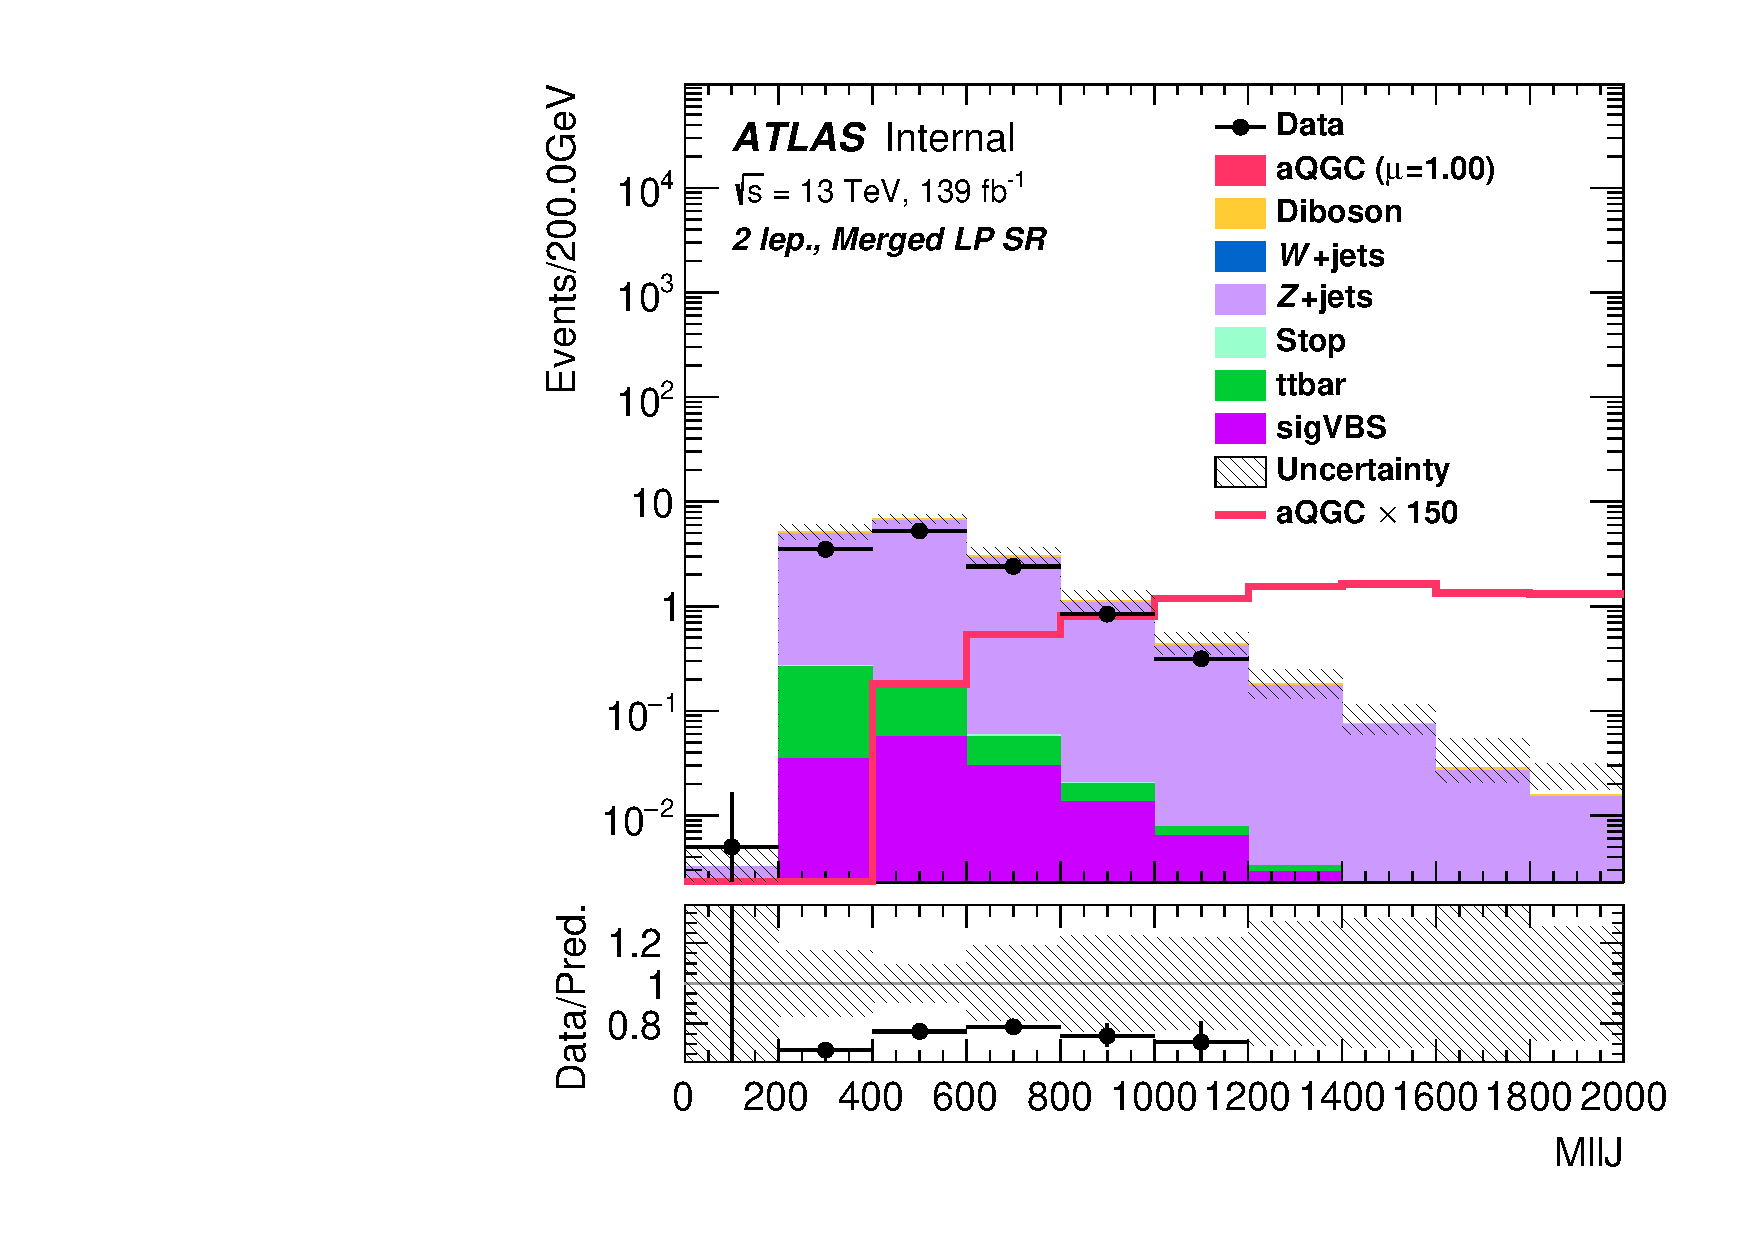
\includegraphics[width=0.32\textwidth]{figures/aQGC/MVV/Region_distMllJ_DSRVBSLP_BMin0_J0_incJet1_L2_T0_incFat1_Y6051_incTag1_Fat1_Prefitlog.pdf}
  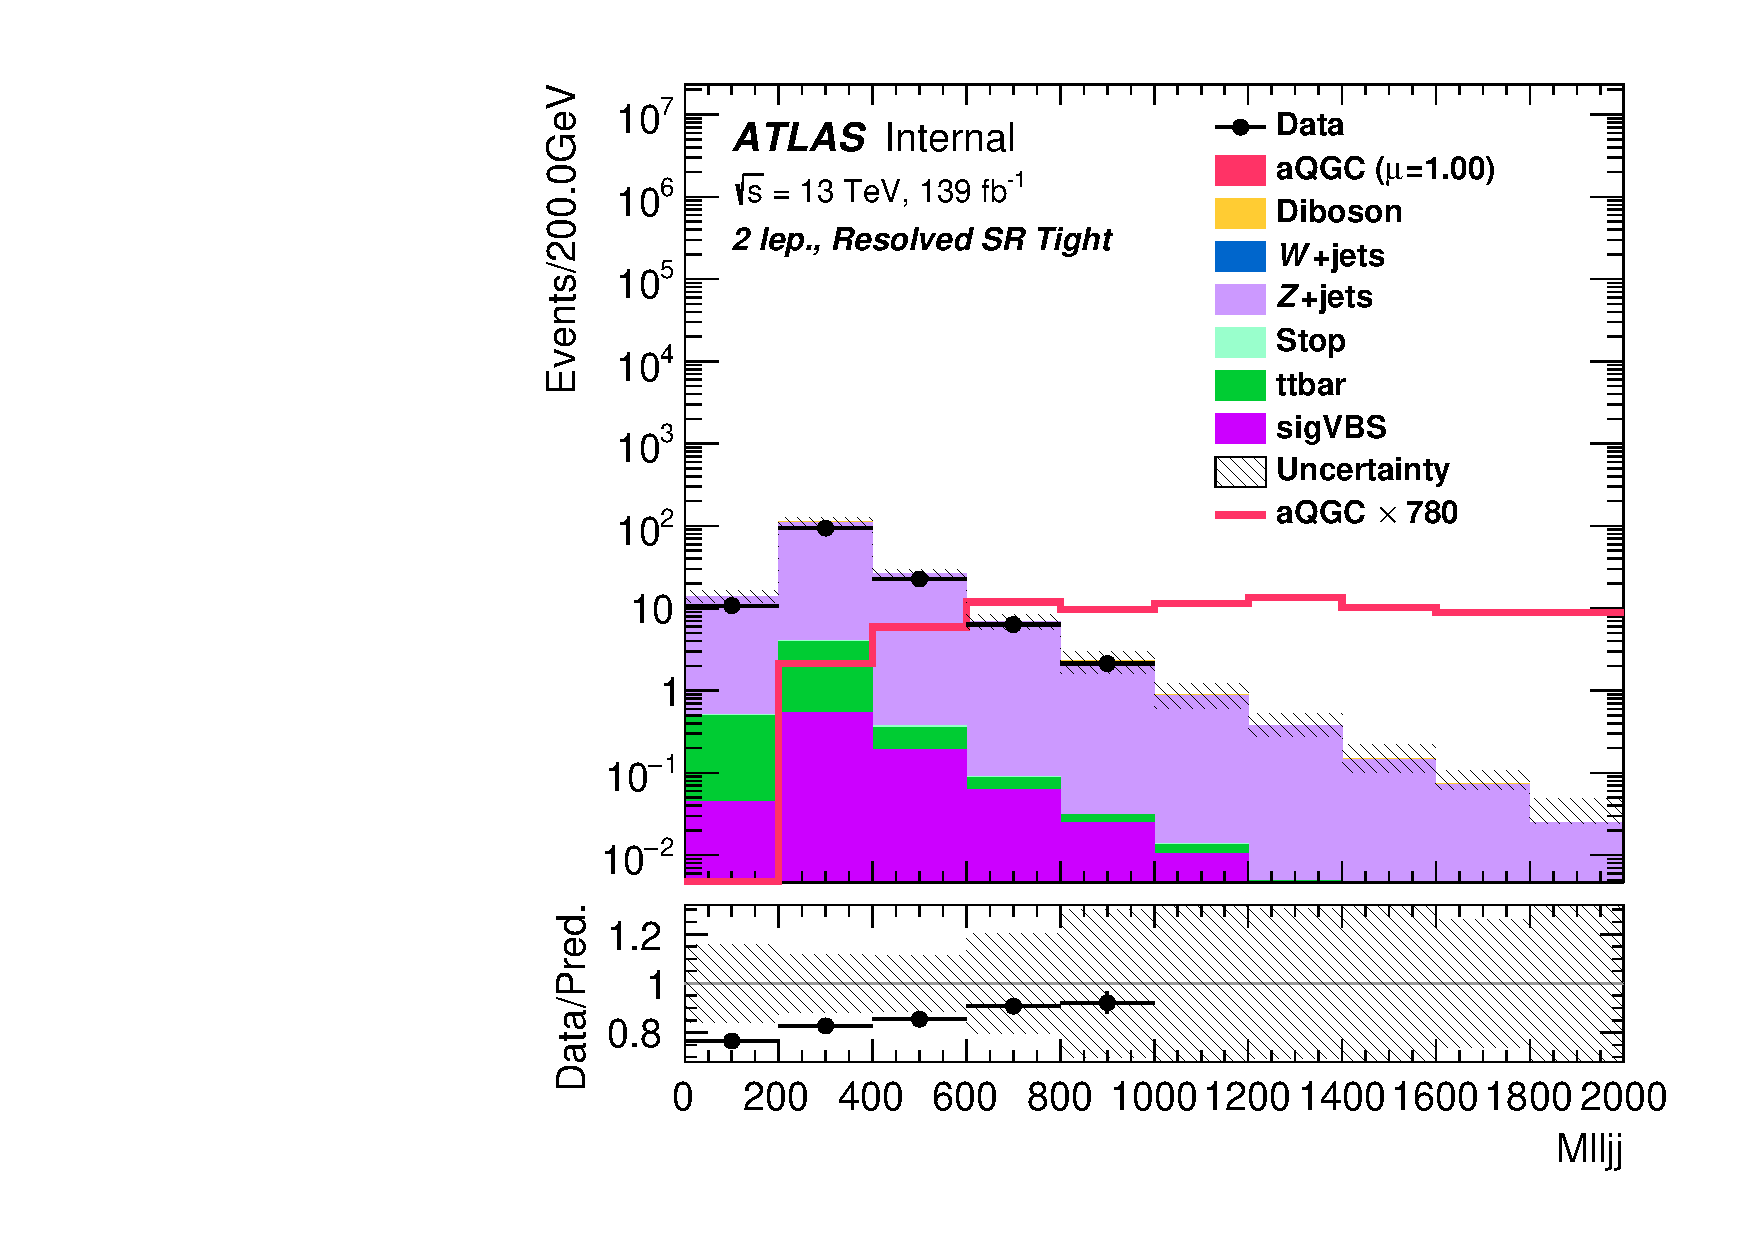
\includegraphics[width=0.32\textwidth]{figures/aQGC/MVV/Region_distMlljj_DSRVBSFid_BMin0_T0_Y6051_incTag1_J2_L2_incJet1_Prefitlog.pdf}
    	%\subfigure[ 1lep HP SR ]{\includegraphics[width=0.32\textwidth]{figures/aQGC/MVV/}}
    	%\subfigure[ 1lep LP SR ]{\includegraphics[width=0.32\textwidth]{figures/aQGC/MVV/}}
    	%\subfigure[ 1lep Fid SR ]{\includegraphics[width=0.32\textwidth]{figures/aQGC/MVV/}}
    	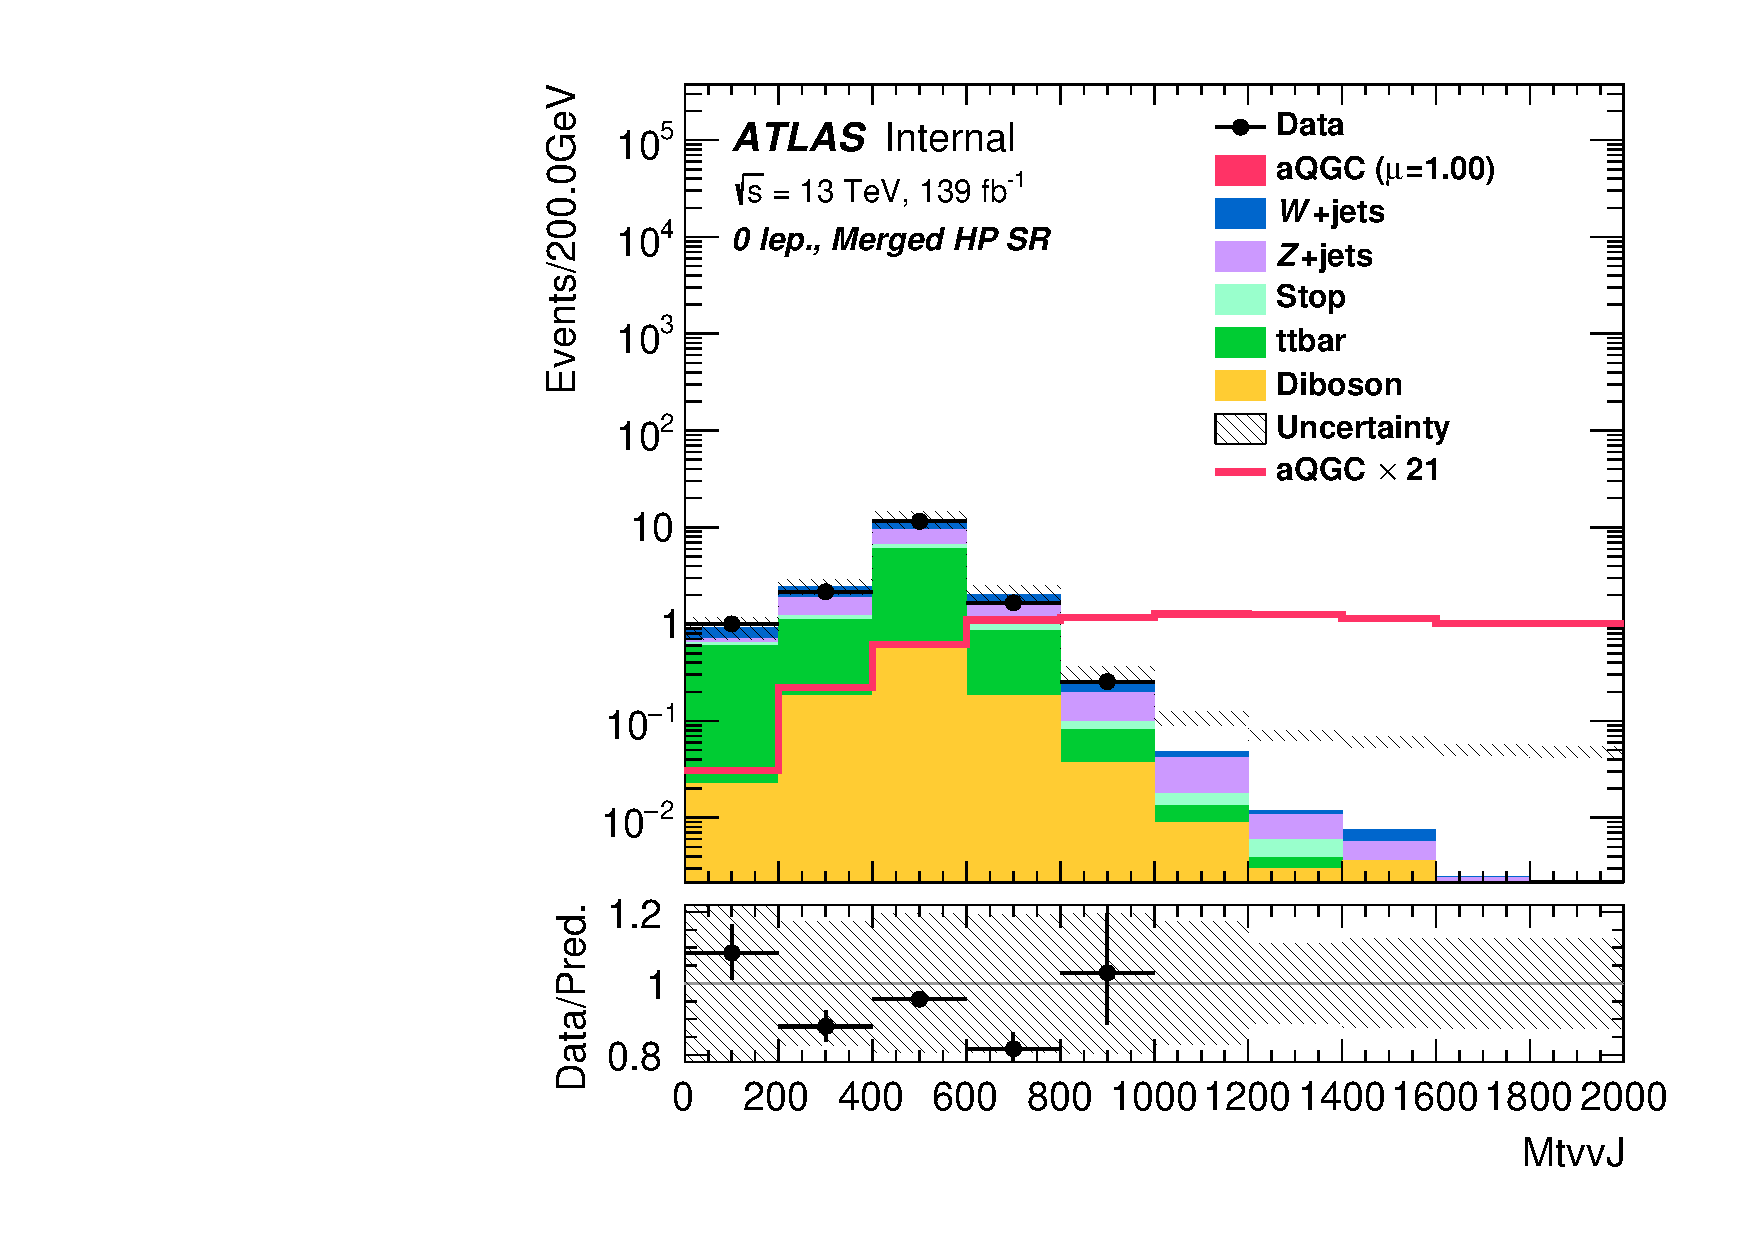
\includegraphics[width=0.32\textwidth]{figures/aQGC/MVV/Region_distMtvvJ_DSRVBSHP_BMin0_J0_incJet1_L0_T0_incFat1_Y6051_incTag1_Fat1_Prefitlog.pdf}
    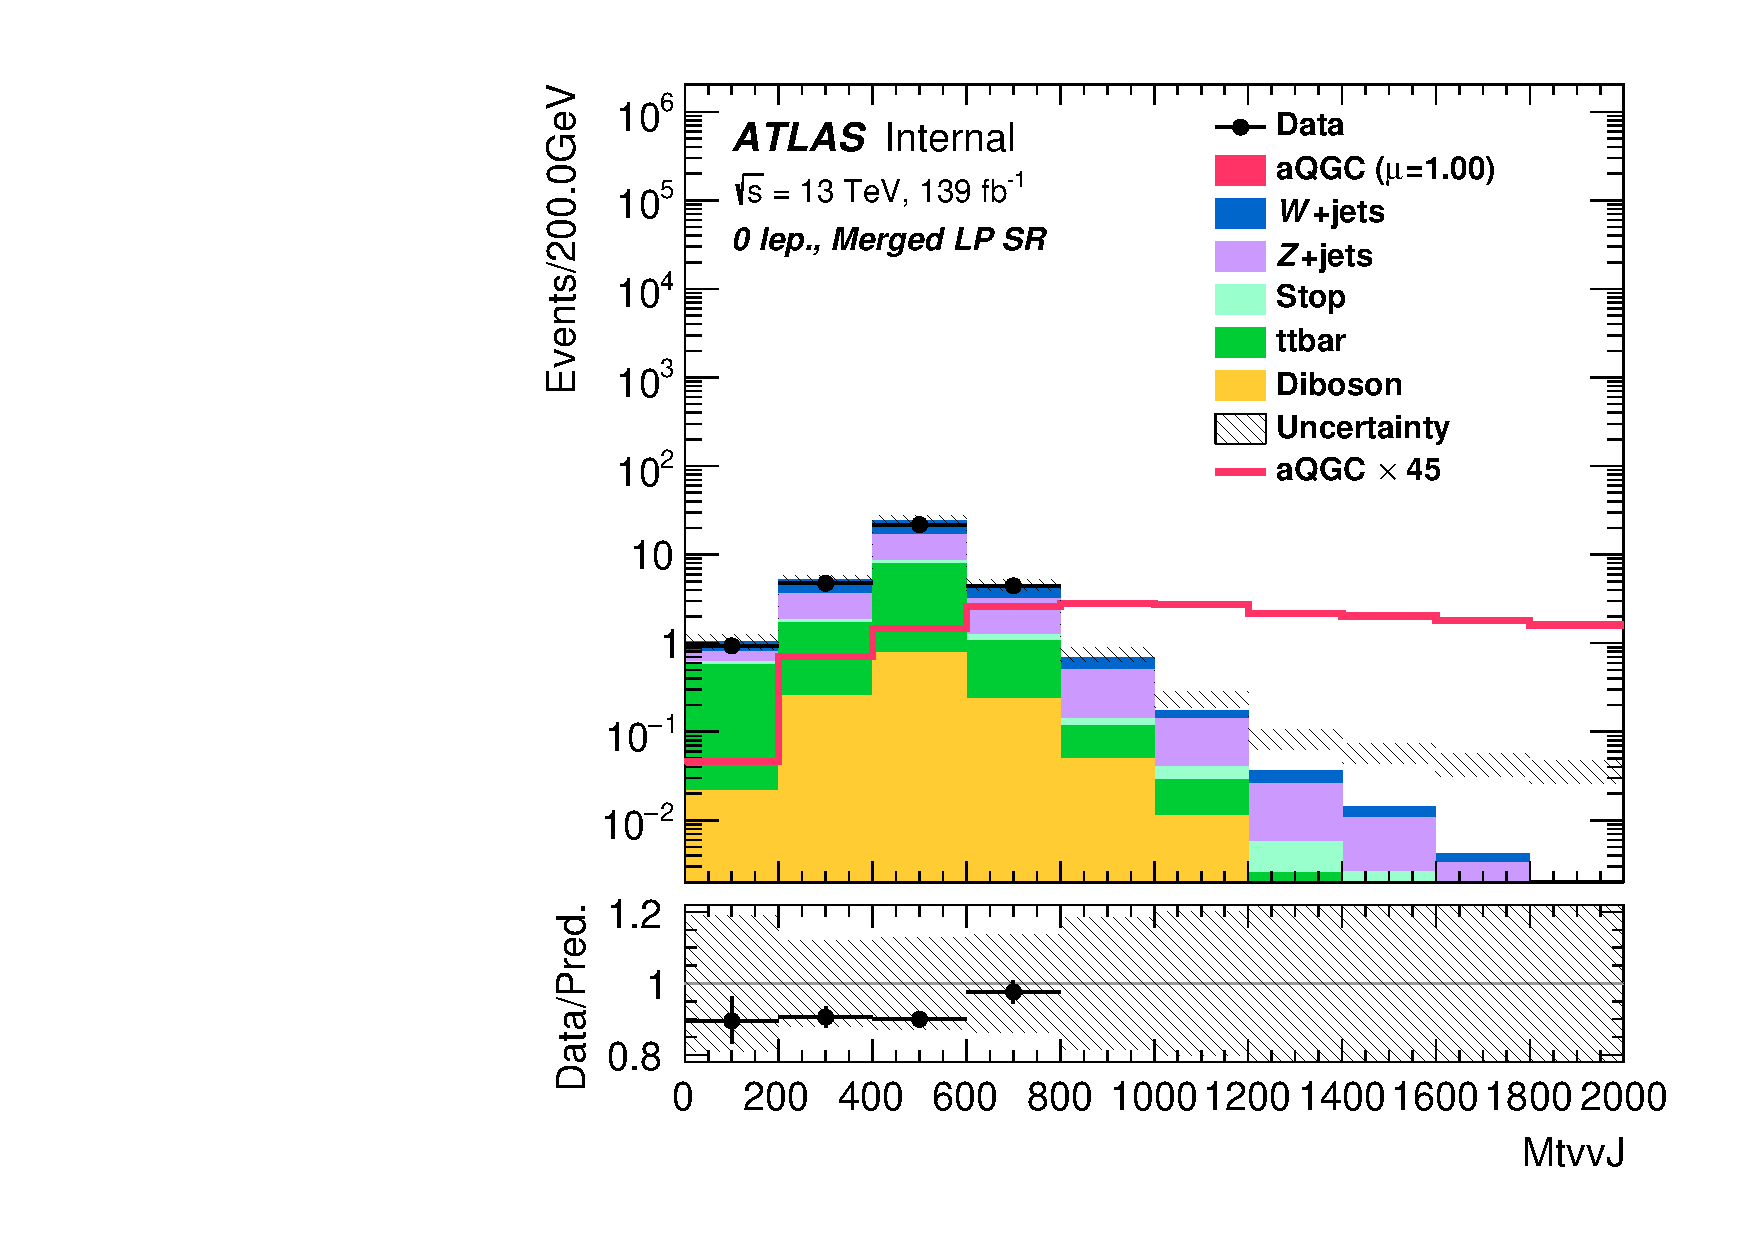
\includegraphics[width=0.32\textwidth]{figures/aQGC/MVV/Region_distMtvvJ_DSRVBSLP_BMin0_J0_incJet1_L0_T0_incFat1_Y6051_incTag1_Fat1_Prefitlog.pdf}
 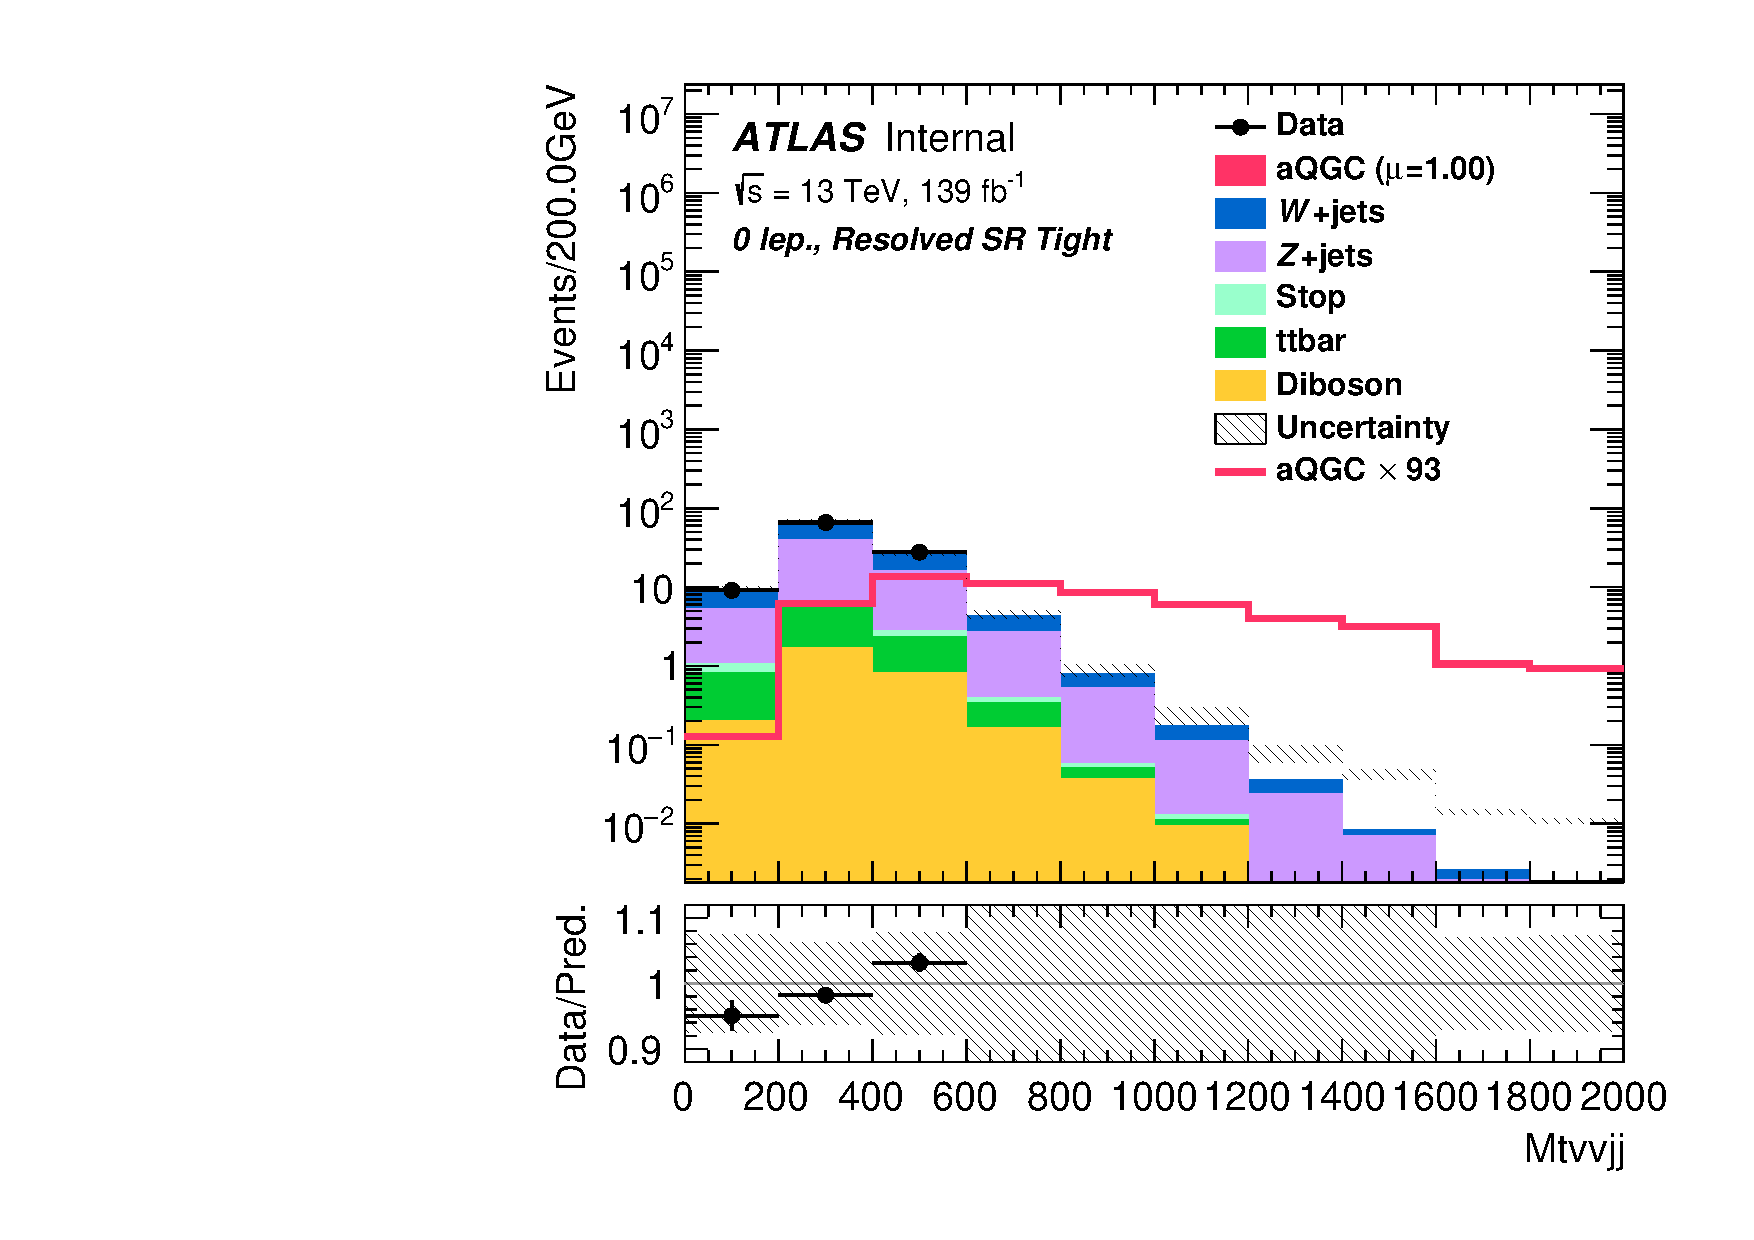
\includegraphics[width=0.32\textwidth]{figures/aQGC/MVV/Region_distMtvvjj_DSRVBSFid_BMin0_T0_Y6051_incTag1_J2_L0_incJet1_Prefitlog.pdf}
        \caption{fig: $m_{VV}$ distribution for \tlep\ (left) and Mtv distribution for \zlep\ (right)}
        \label{fig:mVVdist}
\end{figure}

\begin{table}[ht!]
\small
\begin{center}
%\resizebox{0.9\textwidth}{!}{
\begin{tabular}{ | l || l | l | l |}
\hline
Threshold values (GeV)          & SRVBS\_HP  & SRVBS\_LP & SRVBS\_Fid  \tabularnewline \hline
0-lepton & 1050      & 1200     & 1200       \tabularnewline \hline
1-lepton & 1500      & 1500     & 1500       \tabularnewline \hline
2-lepton & 1500      & 1500     & 1500       \tabularnewline \hline
\end{tabular}
\caption{Threshold values}
\label{tab:2binthreshold}
\end{center}
\end{table}

\section{Limits setting}
Finally, by using both quadratic and interference terms as a combined signal template, the expected 95\% CL upper and lower limits are obtained by the fit to the asimov dataset constructed from the background plus SM EW VV+jj samples, as well as observed limits with data.
All SRs in \zlep, \olep\, and \tlep\ channels are separated into low- and high-$m_{VV}$ bins as discussed in Section~\ref{subsec:2binapproach} and combined statistically.
All systematic uncertainties discussed for Standard Model measurement are included in the fitting.
The SM EW VV+jj signal samples are added to the background as a free floated normalization factor, and all the analysis regions are correlated with EW VV+jj signal samplee.
Due to the small statistics in high-$m_{VV}$ regions compared with the low-$m_{VV}$ regions, the overall behaviors of the post-fit nuisance parameters are almost the same as the SM measurement.
The expected on observed limits are shown at 5 clipping energy points of [1.5, 2.0, 3.0, 5.0, $\infty$]~TeV in Figure~\ref{fig:aQGClimits}.
The unitarity bound from the theoretical calculation \cite{PhysRevD.101.113003} is overlaid.
%The upper and lower limits correspond to the signal hypotheses showing $\Delta NLL \sim \frac{1}{2}\chi^2 = 1.0$.

The log-likelihood (-2 ln $\lambda$; $\lambda$ is a likelihood ratio) distributions with respect to the signal strength of aQGC signal, $\mu_{\mathrm{aQGC}}$, is shown in figure~\ref{fig:ProfileLL},\ref{fig:ProfileLLFS}, \ref{fig:ProfileLLFM} for FT0, FS02, FM0 operator, for each clipping energy of 1500~GeV, 2000~GeV, $\infty$.
%Figure~\ref{}, \ref{}, \ref{} show the log-likelihood curve obtained by the fitting with observed data for each clipping energy, for FT0, FS02, FM0 operators, respectively.
\begin{figure}[ht]
    \centering
    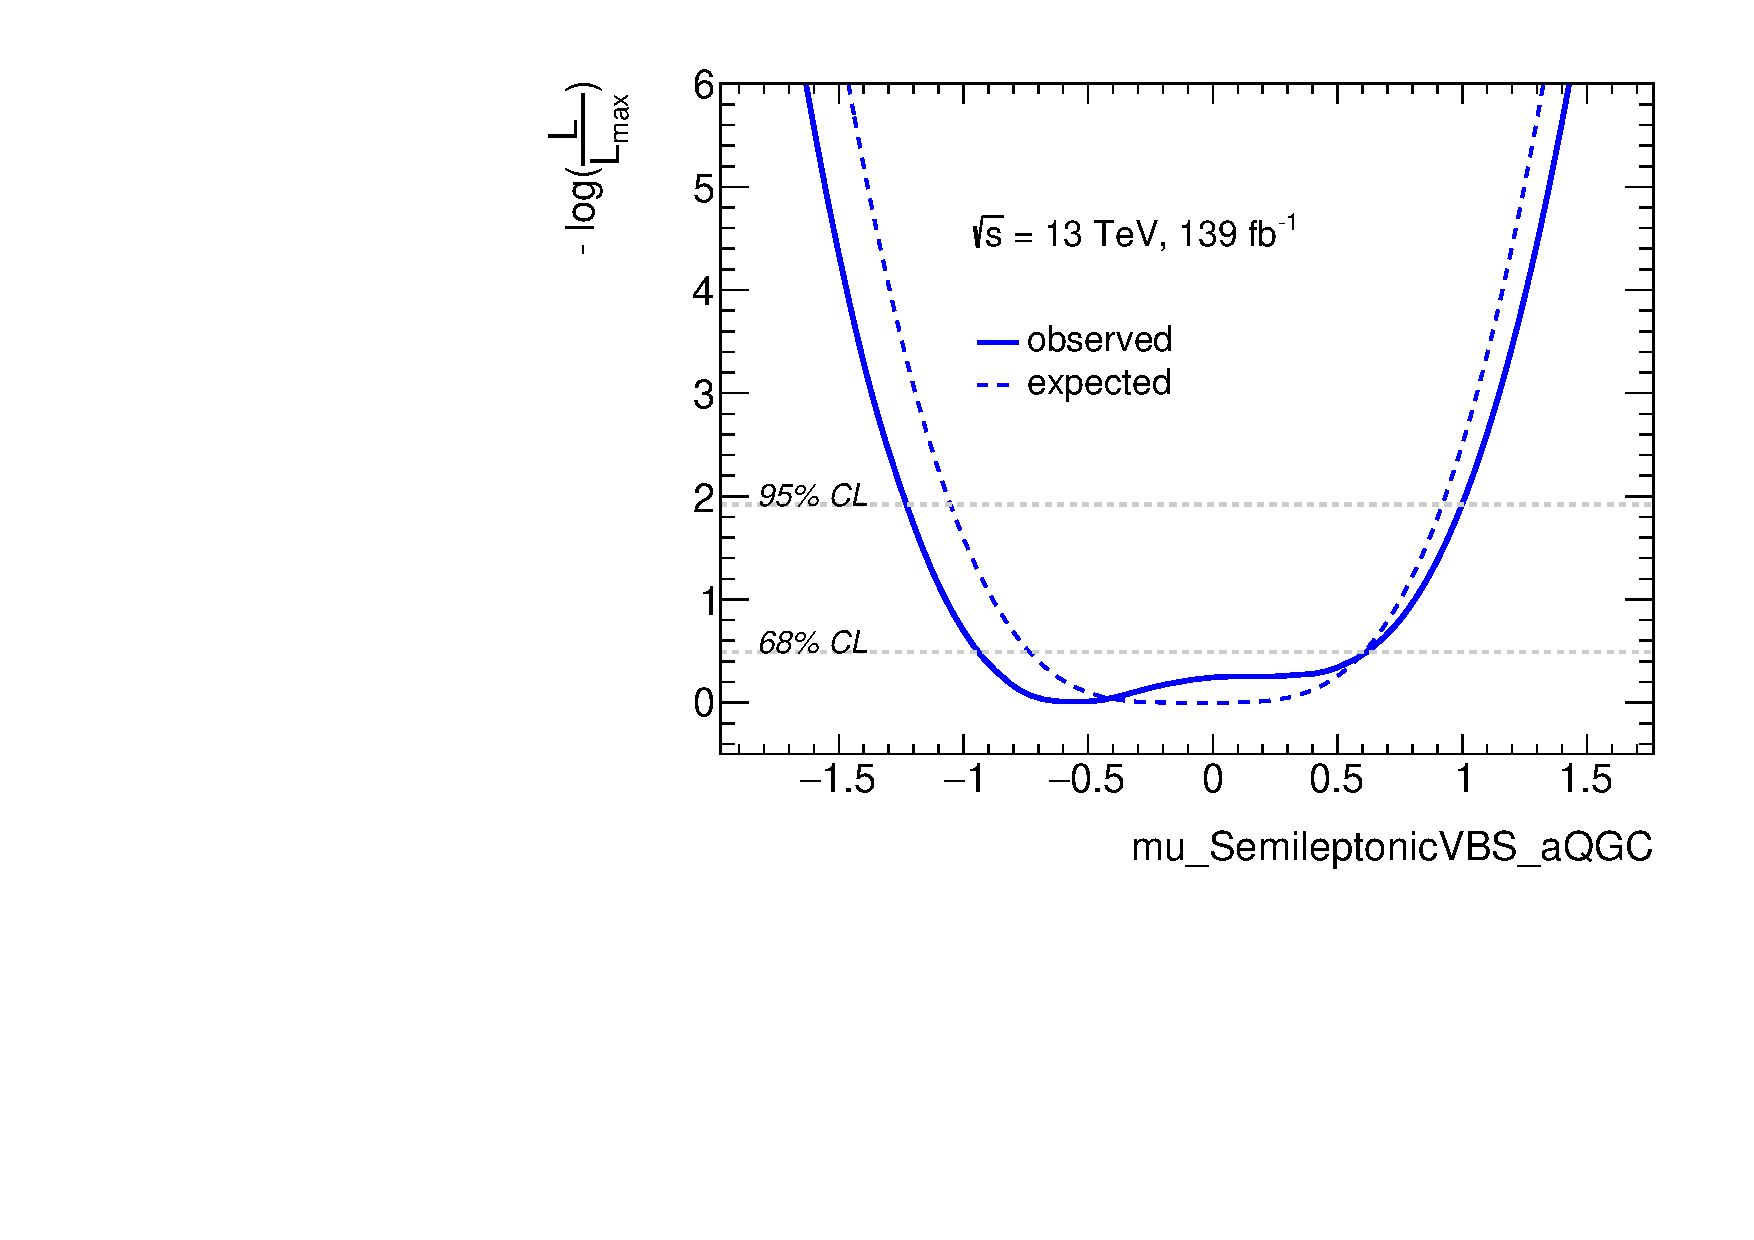
\includegraphics[width=0.32\textwidth]{figures/aQGC/profileFT01500}
    	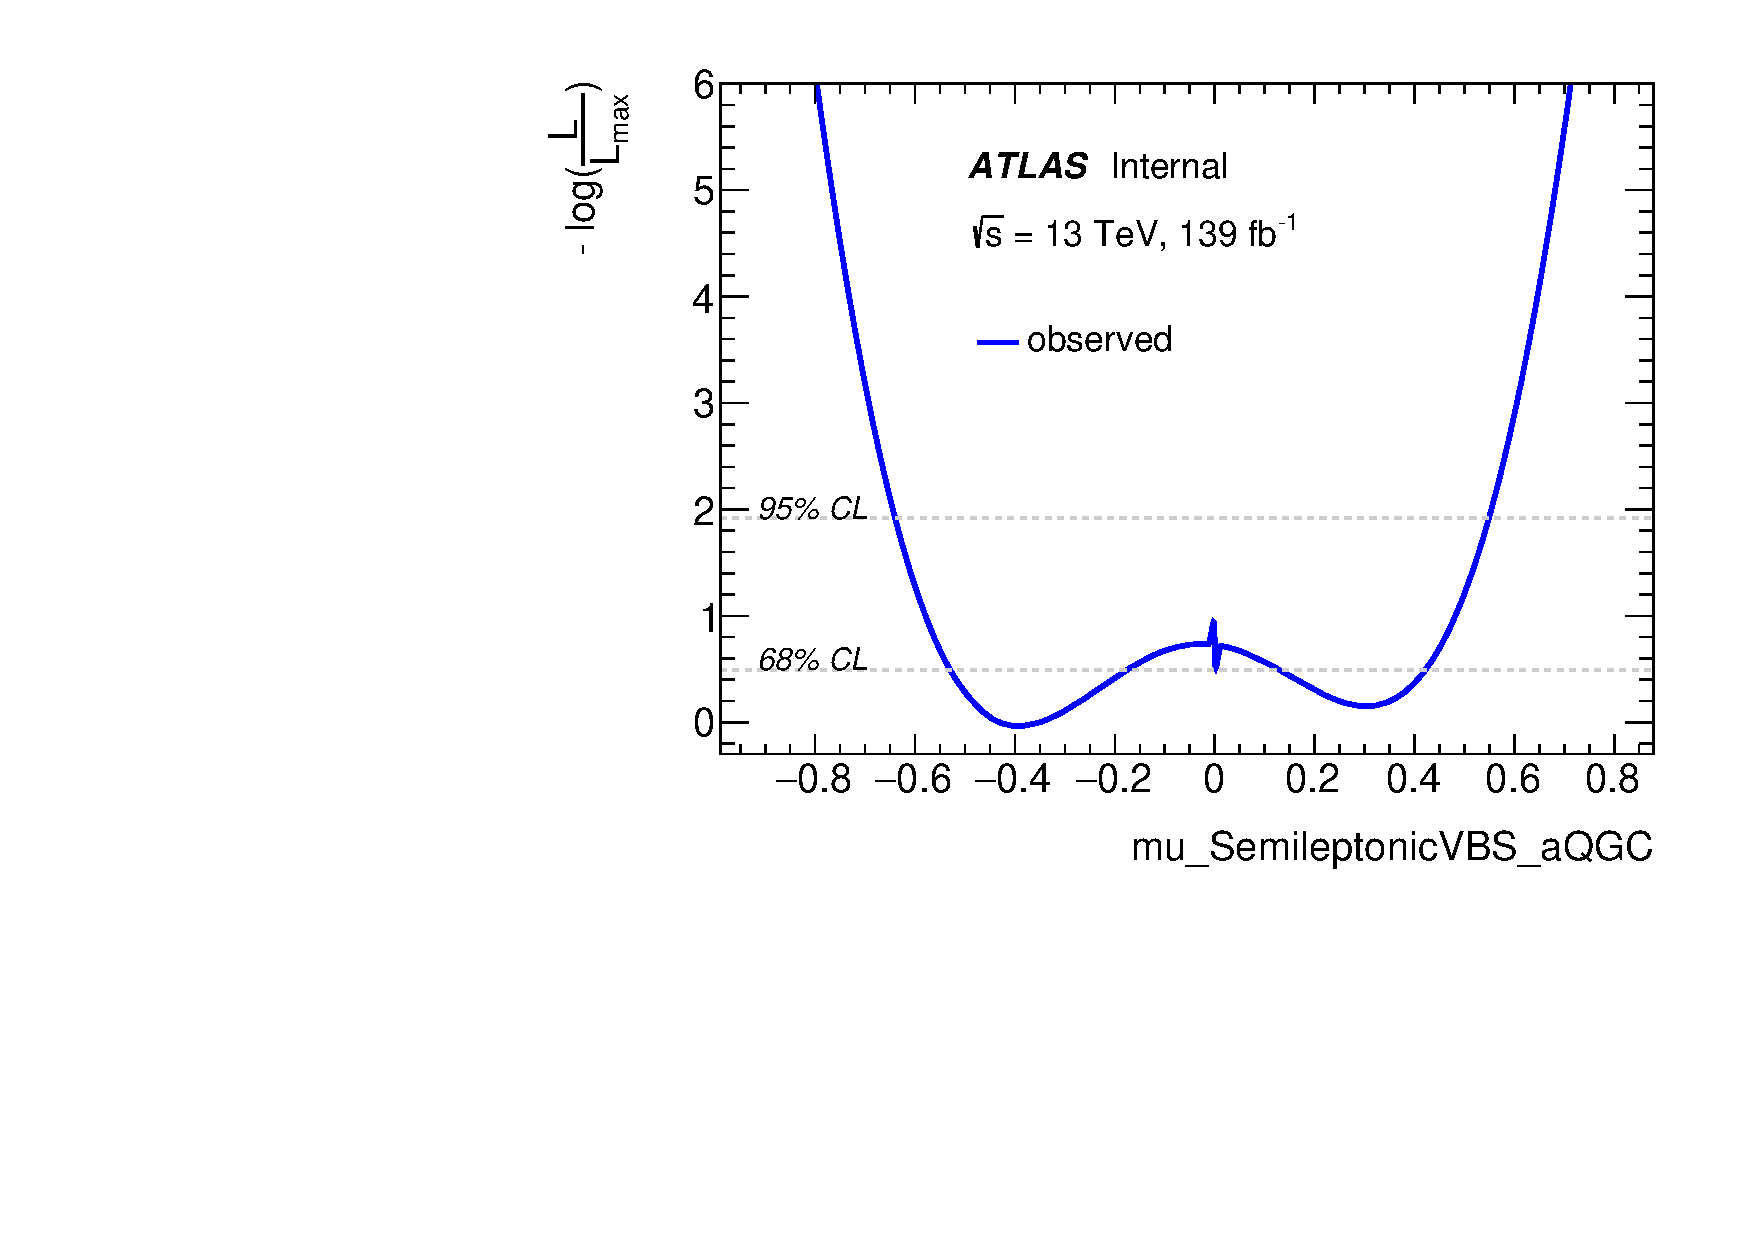
\includegraphics[width=0.32\textwidth]{figures/aQGC/profileFT02000}
    	%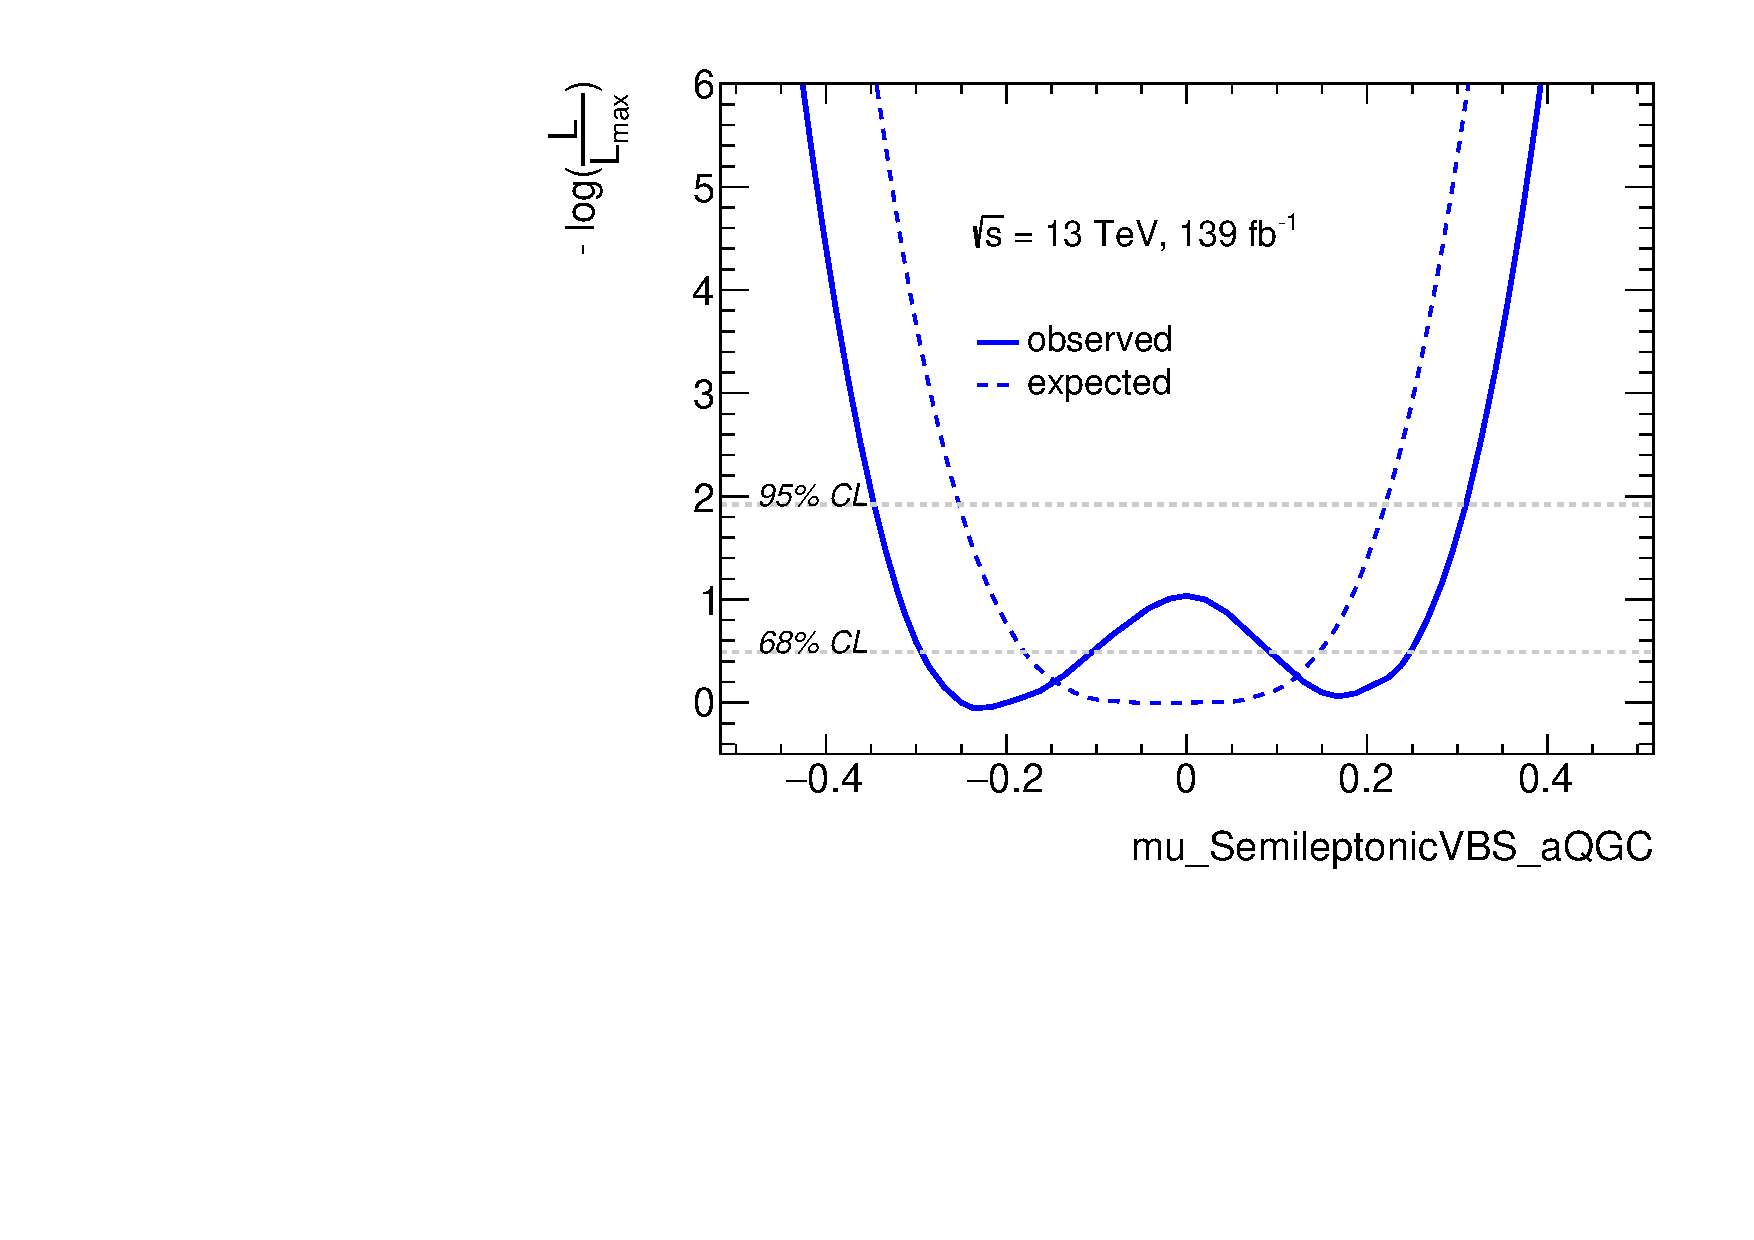
\includegraphics[width=0.38\textwidth]{figures/aQGC/profileFT03000}
        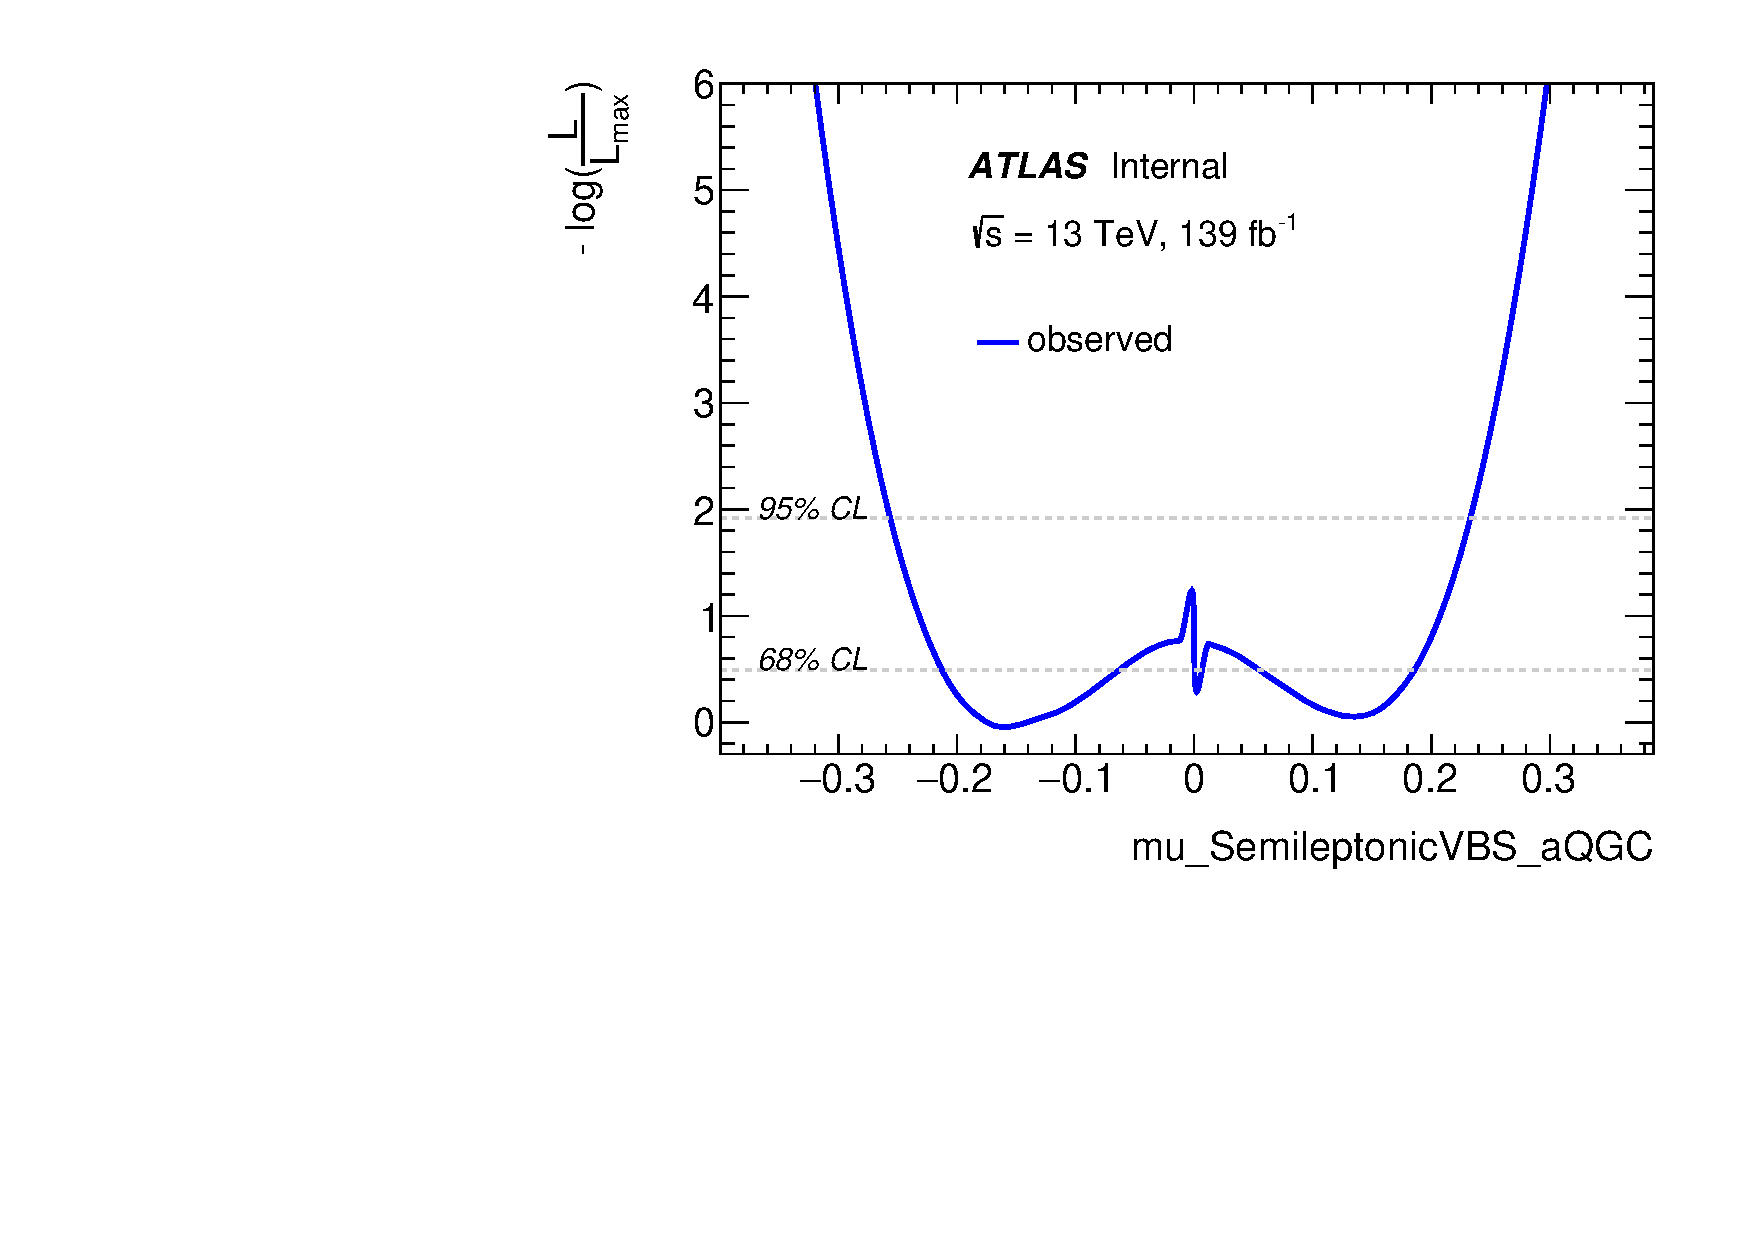
\includegraphics[width=0.32\textwidth]{figures/aQGC/profileFT0inf}
        \caption{The observed log-likelihood curves of FT0 Wilson coefficient where the clipping energy is 1.5~TeV (left), 2.0~TeV (middle), $\infty$ (right).}
        \label{fig:ProfileLL}
\end{figure}
\begin{figure}[ht]
    \centering
    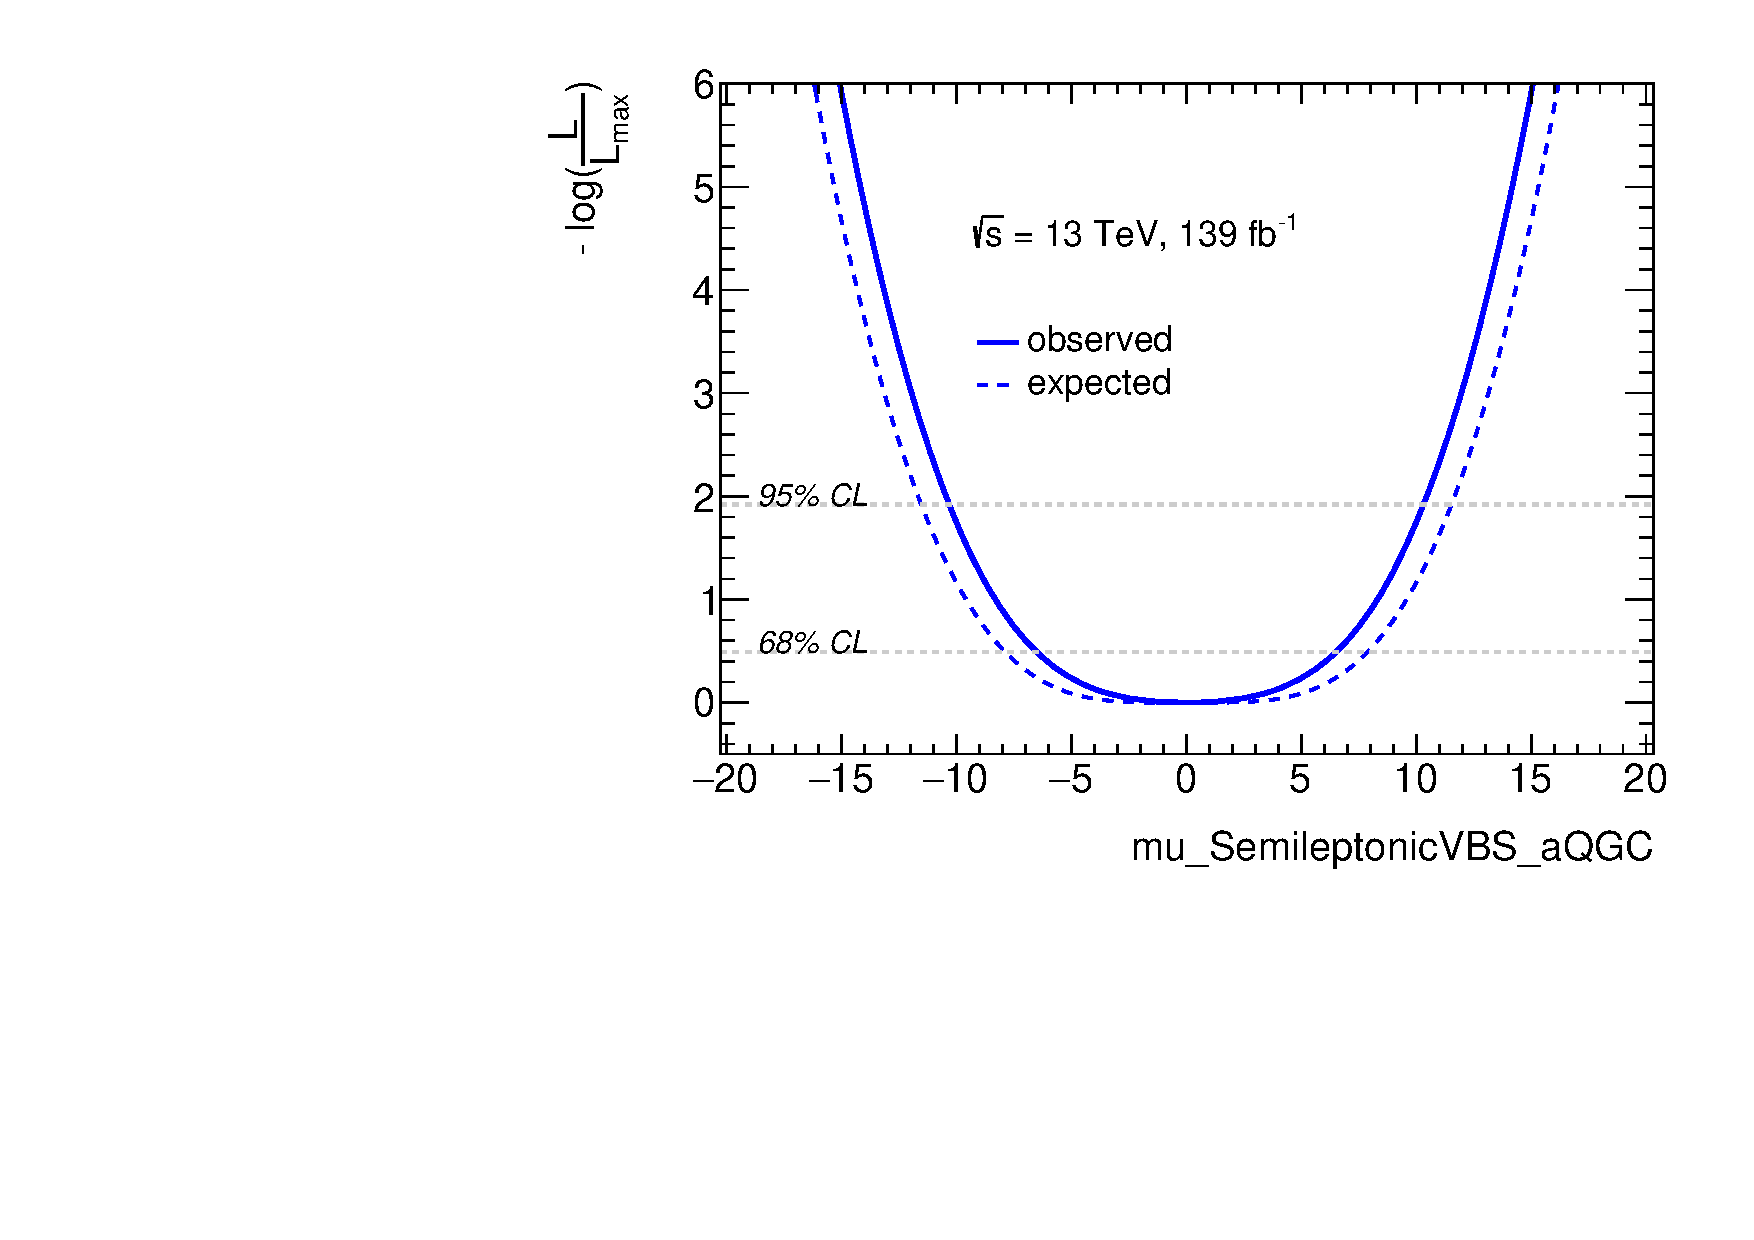
\includegraphics[width=0.32\textwidth]{figures/aQGC/profileFS021500}
    	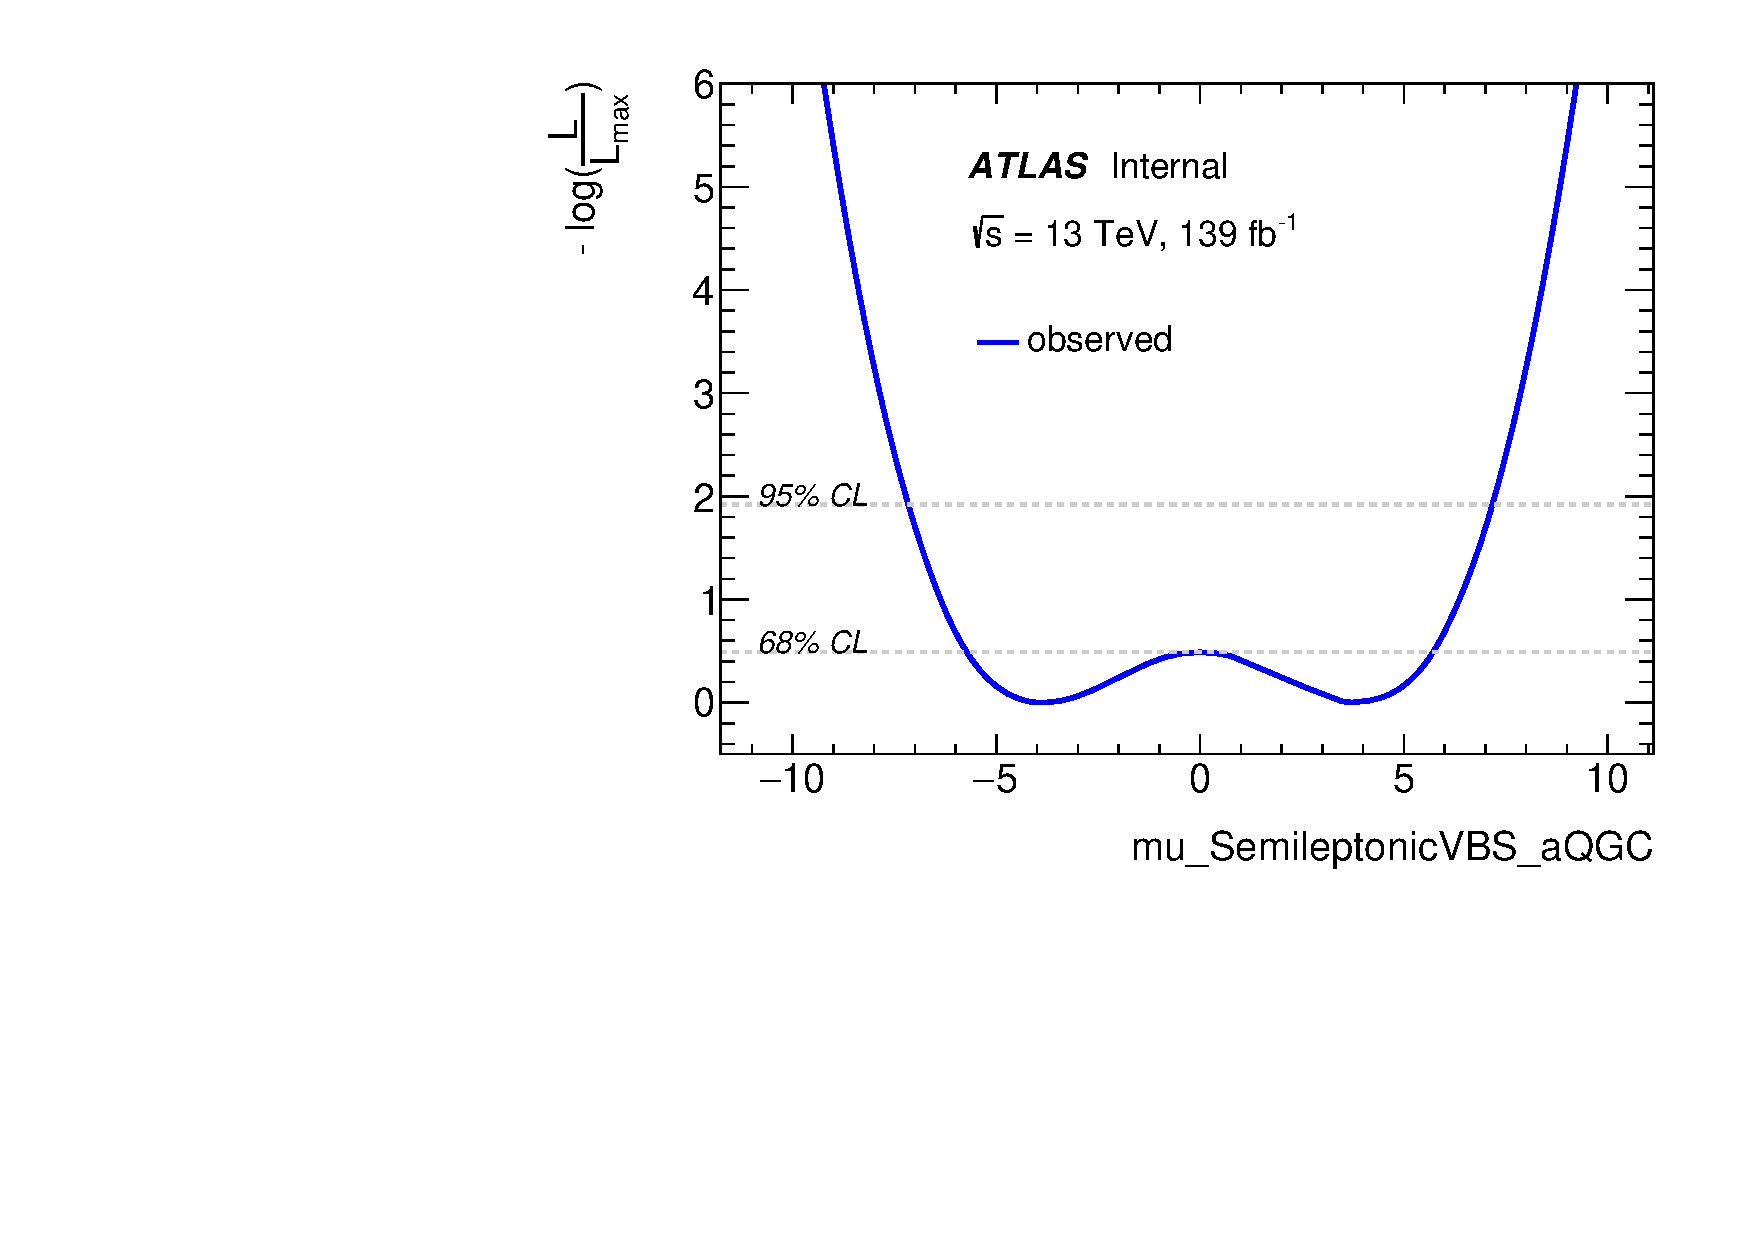
\includegraphics[width=0.32\textwidth]{figures/aQGC/profileFS022000}
    	%\includegraphics[width=0.38\textwidth]{figures/aQGC/profileFS023000}
        \includegraphics[width=0.32\textwidth]{figures/aQGC/profileFS02inf}
        \caption{The observed log-likelihood curves of FS02 Wilson coefficient where the clipping energy is 1.5~TeV (left), 2.0~TeV (middle), $\infty$ (right).}
        \label{fig:ProfileLLFS}
\end{figure}
\begin{figure}[ht]
    \centering
    \includegraphics[width=0.32\textwidth]{figures/aQGC/profileFM01500}
    	\includegraphics[width=0.32\textwidth]{figures/aQGC/profileFM02000}
    	%\includegraphics[width=0.38\textwidth]{figures/aQGC/profileFM03000}
        \includegraphics[width=0.32\textwidth]{figures/aQGC/profileFM0inf}
        \caption{The observed log-likelihood curves of FM0 Wilson coefficient where the clipping energy is 1.5~TeV (left), 2.0~TeV (middle), $\infty$ (right).}
        \label{fig:ProfileLLFM}
\end{figure}
%Figure~\ref{fig:QUADINT} shows the distributions of the quardratic term and the interference term for each FT0, FS02, FM0 operator.
%The quardratic term has large contribution compared to the interference term.
Due to the large contribution of the QUAD term in the parametrization of the $\mu_{\mathrm{aQGC}}$, the log-likelihood curve has two local minimums.
A $\mu_{\mathrm{aQGC}}$ value at crossing the 95\% confidence interval line and the likelihood curve is used to calculate upper and lower limits on the coefficients. 
%The 95\% confidence interval corresponds to 1.9.
For high clipping values, the results exclude the signal strength already excluded by the theoretical unitarity bound.
Table~\ref{tab:aQGClimits} shows the uniterized and ununiterized expected and observed limits from figure~\ref{fig:aQGClimits}, where uniterized limit is the intersection point of the theoretical unitality bound and experimental limit line, while ununiterized limit is the limit with no clipping energy.
\begin{figure}[ht]
    \centering
    \includegraphics[width=0.45\textwidth]{figures/aQGC/ClippedFT0CI.pdf}
    	\includegraphics[width=0.45\textwidth]{figures/aQGC/ClippedFM0CI.pdf}
    	\includegraphics[width=0.45\textwidth]{figures/aQGC/ClippedFS02CI.pdf}
        \caption{Expected limits (green) and observed limits (blue) for 5 clipping points are shown for each Wilson coefficient FT0 (left), FM0 (right), FS02 (middle). The black line is the theoretical unitarity bound.}
        \label{fig:aQGClimits}
\end{figure}

%\begin{table}[ht!]
%\small
%\begin{center}
%%\resizebox{0.9\textwidth}{!}{
%\begin{tabular}{ | l || l | l | l | l | l |}
%\hline
%                   & 1.5 [ TeV ] & 2.0 [ TeV ] & 3.0 [ TeV ] & 5.0 [ TeV ] & $\infty$                  \tabularnewline \hline
%FT0                & [ -1.02, 0.88 ]  & [ -0.47, 0.41 ]  & [ -0.25, 0.21 ]  & [ -0.16, 0.15 ]  & [ -0.16, 0.16 ]              \tabularnewline \hline
%FM0                & [ -5.63, 5.62 ]  & [ -2.47, 2.47 ]  & [ -1.37, 1.37 ]  & [ -1.08, 1.09 ]  & [ -1.06, 1.07 ]              \tabularnewline \hline

%\caption{Expected limits for each clipping point. Ununiterized limit is shown as the limit with no clipping energy, labeled as $\infty$ in figure~\ref{fig:aQGClimits}.}
%\label{tab:aQGClimits}
%\end{center}
%\end{table}

%uniterized limit
\begin{table}[ht!]
\small
\begin{center}
\resizebox{0.9\textwidth}{!}{
\begin{tabular}{ | l || l | l | l | l | }
\hline
                   & \multicolumn{2}{|l|}{expected limit}                      & \multicolumn{2}{|l|}{observed limit} \tabularnewline \hline
Wilson coefficient & uniterized                             & ununiterized     & uniterized                            & ununiterized \tabularnewline \hline
FT0                & [ -0.48, 0.39 ] at [ 1.99, 2.09 ]~TeV  & [ -0.16, 0.16 ]  & [ -1.04, 0.74 ] at [ 1.64, 1.78 ]~TeV & [ -0.25, 0.23 ]\tabularnewline \hline
FT1                & [  ] at [  ]~TeV  & [ -0.16,0.16 ]     & [  ] at [  ]~TeV & [ -0.24,0.05 ]\tabularnewline \hline
FT2                & [  ] at [  ]~TeV  & [ -0.41,0.41 ]     & [  ] at [  ]~TeV & [ -0.42,0.52 ]\tabularnewline \hline
FT5                & [  ] at [  ]~TeV  & [ -0.53,0.51 ]     & [  ] at [  ]~TeV & [ -0.46,0.62 ]\tabularnewline \hline
FT6                & [  ] at [  ]~TeV  & [ -0.71,0.68 ]     & [  ] at [  ]~TeV & [ -0.71,0.68 ]\tabularnewline \hline
FT7                & [  ] at [  ]~TeV  & [ -1.67,1.50 ]     & [  ] at [  ]~TeV & [ -1.67,1.50 ]\tabularnewline \hline
FT8                & [  ] at [  ]~TeV  & [ -0.56,0.56 ]     & [  ] at [  ]~TeV & [ -0.44,0.47 ]\tabularnewline \hline
FT9                & [  ] at [  ]~TeV  & [ -1.16,1.18 ]     & [  ] at [  ]~TeV & [ -1.02,0.94 ]\tabularnewline \hline
FS02               & [ -5.46, 5.61 ] at [ 2.05, 2.07 ]~TeV  & [ -3.27, 3.32 ]  & [ -7.53, 7.80 ] at [ 1.91, 1.90 ]~TeV & [ -3,45, 4.19 ]\tabularnewline \hline
FS1                & [  ] at [  ]~TeV  & [ -6.70,6.74 ]     & [  ] at [  ]~TeV & [ -8.57,8.57 ]\tabularnewline \hline
FM0                & [  ] at [  ]~TeV  & [ -1.06, 1.07 ]    & [ -1.63, 1.63 ] at [ 2.24, 2.24 ]~TeV & [ -1.32, 1.31 ]\tabularnewline \hline
FM1                & [  ] at [  ]~TeV  & [ -3.04,3.05 ]     & [  ] at [  ]~TeV & [ -4.01,4.07 ]\tabularnewline \hline
FM2                & [  ] at [  ]~TeV  & [ -1.57,1.57 ]     & [  ] at [  ]~TeV & [ -1.94,1.94 ]\tabularnewline \hline
FM3                & [  ] at [  ]~TeV  & [ -5.02,5.01 ]     & [  ] at [  ]~TeV & [ -5.93,6.00 ]\tabularnewline \hline
FM4                & [  ] at [  ]~TeV  & [ -2.36,2.45 ]     & [  ] at [  ]~TeV & [ -3.10,3.10 ]\tabularnewline \hline
FM5                & [  ] at [  ]~TeV  & [ -3.62,3.62 ]     & [  ] at [  ]~TeV & [ -4.60,4.61 ]\tabularnewline \hline
FM7                & [  ] at [  ]~TeV  & [ -4.99,4.88 ]     & [  ] at [  ]~TeV & [ -6.75,6.62 ]\tabularnewline \hline
\end{tabular}
}
\caption{Uniterized and ununiterized expected limits and observed limits. Uniterized limit is the intersection point of the theoretical unitality bound and experimental limit line. Ununiterized limit is the limit with no clipping energy, labeled as $\infty$ in figure~\ref{fig:aQGClimits}.}
\label{tab:aQGClimits}
\end{center}
\end{table}

%The ununiterized limits can be compared with results of other analyses.
%%Compared to the figure~\ref{fig:limitFT},\ref{fig:limitFM}, \ref{fig:limitFS}, these results give the
%The same procedure is performed with all 17 Wilson coefficient.
%The uniterized expected limit and the ununiterized expected limit is plotted in figure~\ref{}.



\chapter{Results}

\chapter{Conclusions}

%Conclusion will be put here



\chapter*{Acknowledgement}

I would first like to express my gratitude to Gi-Chol Cho, Testuo Deguchi, Minoru Soda, and Koji Terashi for accepting the role of being part of my jury. 
I am grateful for the constructive discussions during the defense and the comments on the manuscript.

I would like to express my gratitude to my supervisor, Takanori Kono, for giving me lots of opportunities and for many supports through the various tasks.

I am grateful to Lydia Fayard, for making my visit possible to the IJCLab and for welcoming me with lots of academic discussions. It was really fortunate for me to have a chance to work with people in the IJCLab group who have great expertise. I would like to express special thanks to Jean-Francois Grivaz, for earnestly helping us to improve the VBS analysis with his expertise.  

Through collaboration on the analysis, I appreciate a lot to the whole VBS team for giving me much advice, and for getting over the problem together. I would like to thank especially the convener, Dimitris Varouchas for giving me lots of advice from the basics, and Antonio Giannini for consulting my tasks.

I would like to deeply thank Takuya Nobe, for his great guidance and help in many aspects of the analysis through countless discussions.

I really appreciate all my colleagues from Ochanomizu University, from the IJCLab,  and from the ATLAS Japan group who worked with me.
It was a great pleasure collaborating with all of them, who made my experience enjoyable. 

I also would like the thank my friends who chatted with me and helped me get through my Ph.D. days.

Finally, I would like to express my biggest thank you to my parents.

  


\bibliography{}


%bibliography
%\bibliography{bib/ATLAS}
%\bibliography{bib/CMS}
%\bibliography{bib/PubNotes}
%\bibliography{bib/ConfNotes}

\appendix

\listoffigures
\listoftables

\end{document}

